\chapter{Dinámica de la partícula. Campos de fuerza}	
\chaptermark{Dinámica de la partícula}

La dinámica es una parte de la mecánica en que, dadas unas condiciones, se estudia qué movimiento se va a producir.

Consideraciones: En mecánica clásica el \emph{espacio} es como un gran cajón donde está todo el universo físico. El \emph{tiempo} es absoluto: dados dos fenómenos, todos los relojes de todos los posibles observadores medirán lo mismo.

\rule{150pt}{0.4pt} 

Los fenómenos mecánicos se describen mediante sistemas de referencia basados en los conceptos de espacio y tiempo. Por su importancia conviene enunciar los postulados que asume la mecánica clásica para estos conceptos. 

El \emph{espacio}, y por tanto su métrica, tiene las propiedades siguientes. 
\begin{itemize}
\vspace{-2mm}\item Independencia de los objetos en él inmersos. (La métrica del espacio no se ve afectada por los mismos.) 
\vspace{-2mm}\item Constancia a lo largo del tiempo. 
\vspace{-2mm}\item \textbf{Homogeneidad: es igual en todos los puntos}, no existiendo puntos privilegiados. 
\vspace{-2mm}\item \textbf{Isotropía: es igual en todas las direcciones}, no existiendo direcciones privilegiadas. 
\end{itemize}
El espacio se caracteriza por una métrica euclídea:
 
$d(\;(x_1,y_1,z_1)\;(x_2,y_2,z_2)\;)=\sqrt{(x_2-x_1)^2+(y_2-y_1)^2+(z_2-z_1)^2}$ 

El \emph{tiempo} se caracteriza a su vez por las siguientes propiedades. 
\begin{itemize}
\vspace{-2mm}\item \textbf{Homogeneidad}, al no existir instantes privilegiados. 
\vspace{-2mm}\item Fluye constantemente en un sentido, por lo que no se puede retroceder ni volver al pasado. Asimismo, los fenómenos futuros no pueden condicionar los presentes. \textbf{No} se cumple por tanto la \textbf{isotropía}, existiendo un único sentido en el que puede discurrir el tiempo. 
\vspace{-2mm}\item \textbf{Simultaneidad absoluta}: Los fenómenos considerados simultáneos para dos observadores en sendos sistemas de referencia lo son asimismo para cualquier otro observador ligado a cualquier otro sistema de referencia. 
\end{itemize}

\setlength{\parindent}{0pt} %Aparecía sangrado en 1a linea, esto lo evita
En mecánica clásica, el tiempo se considera una variable de naturaleza distinta de las variables espaciales y la métrica euclídea no está influenciada por él. 

Algunos de estos postulados básicos no son aceptados por la mecánica relativista. La teoría de la relatividad restringida establece una referencia en cuatro dimensiones espacio-tiempo. La teoría de la relatividad general establece un espacio curvado, con métrica riemanniana no euclídea, debido a la presencia de masas que condicionan dicha métrica. De esta forma el espacio no sería independiente de los objetos en él inmersos 

\rule{150pt}{0.4pt} 

Una vía para abordar los problemas de la mecánica es averiguar las `causas del movimiento': ``el \emph{movimiento} es debido a la \emph{interacción} que se ejerce entre las diversas partes o cuerpos de universo''.


\section{Leyes del movimiento. Newton (3)}

\begin{cita}
``Si he visto más lejos que los demás es porque estoy sentado sobre los hombros de gigantes'' (Isaac Newton).
\end{cita} 

\vspace{-13mm}\scriptsize{Isaac Newton (1643-1727) escribió esa frase en una carta a Robert Hooke en la que hacía mención a sus predecesores Copérnico, Galileo y Kepler}\normalsize{.}

\vspace{4mm}A las entidades responsables de que los cuerpos varíen su posición en el espacio absoluto newtoniano les llamaremos \emph{interacciones} o \emph{fuerzas.}

En el siglo $XVIII$, Newton postula las tres leyes de la mecánica clásica.

\vspace{3mm}
\begin{miparrafo}

\textbf{1. } \emph{``Todo cuerpo permanece en reposo o en movimiento uniforme a menos que se obre sobre él alguna fuerza''.} Es la llamada \textsf{Ley de Inercia.}

\textbf{2. } \emph{``Todo cuerpo sobre el que actúa una fuerza se mueve de forma tal que la variación de su cantidad de movimiento por unidad de tiempo es igual a la fuerza''.} \textsf{Fuerza igual a masa por aceleración.}

\textbf{3. } \emph{``Cuando dos cuerpos ejercen entre sí fuerzas, éstas son de intensidades iguales y sentidos opuestos y están dirigidas a lo largo de la línea que une a los dos cuerpos considerados como partículas''.} 
\textsf{Ley de Acción y Reacción.}

\end{miparrafo}

En la primera ley se introduce la `fuerza' cualitativamente, en la segunda cuantitativamente.

Hemos introducido una nueva magnitud, la \emph{cantidad de movimiento}, 

\begin{equation}
\label{cant-mov}
\subrayado{\vec p=m\; \vec v} \qquad \qquad  \textcolor{gris}{[\vec p]=[\mathrm{MLT}^{-1}]\to \mathrm{kg\ m\ s}^{-1}}
\end{equation}

\begin{equation}
\label{Newton}
\subrayado{\vec F=\dv{\vec p}{t}} 	\qquad \qquad  \textcolor{gris}{[\vec F]=\dfrac{[\vec p]}{[t]}=[\mathrm{MLT}^{-2}]\to \mathrm{kg\ m\ s}^{-2}=\mathrm{N}}
\end{equation}


\emph{Primera hipótesis de la mecánica clásica:} La \emph{masa} es una característica especial de los cuerpos que interaccionan y no varía respecto al tiempo, es \emph{constante}.

\begin{equation}
\label{fma}
 \boldsymbol{ \vec F}=\dv{\vec p}{t}=\dv{(m\; \vec v)}{t}=m\; \dv{\vec v}{t}=\boldsymbol{ m\; \vec a}
\end{equation}


Supongamos dos cuerpos interactuando: $\vec F_1=m_1\ \vec a_1$ y  $\vec F_2=m_2\ \vec a_2$. Supongamos que forman un sistema aislado en el espacio, es decir, el resto de cuerpos del universo ejercen sobre ellos una interacción despreciable.

Por el tercer postulado (ley) de Newton, tenemos: $\vec F_1=-\vec F_2$, es decir, $m_1\; \vec a_1=-m_2\;\vec a_2\;:$
$$\displaystyle \dfrac {m_2}{m_1}=\dfrac {a_1}{a_2}$$
Tomamos un cuerpo cualquiera del universo de masa $m_1$ que no conocemos y, arbitrariamente, le damos el valor de `masa unidad', con lo que para otro cuerpo, $\displaystyle m_2=\dfrac {a_1}{a_2}\; m_1$ y así introducimos el concepto de masa.

\begin{figure}[]
		\centering
		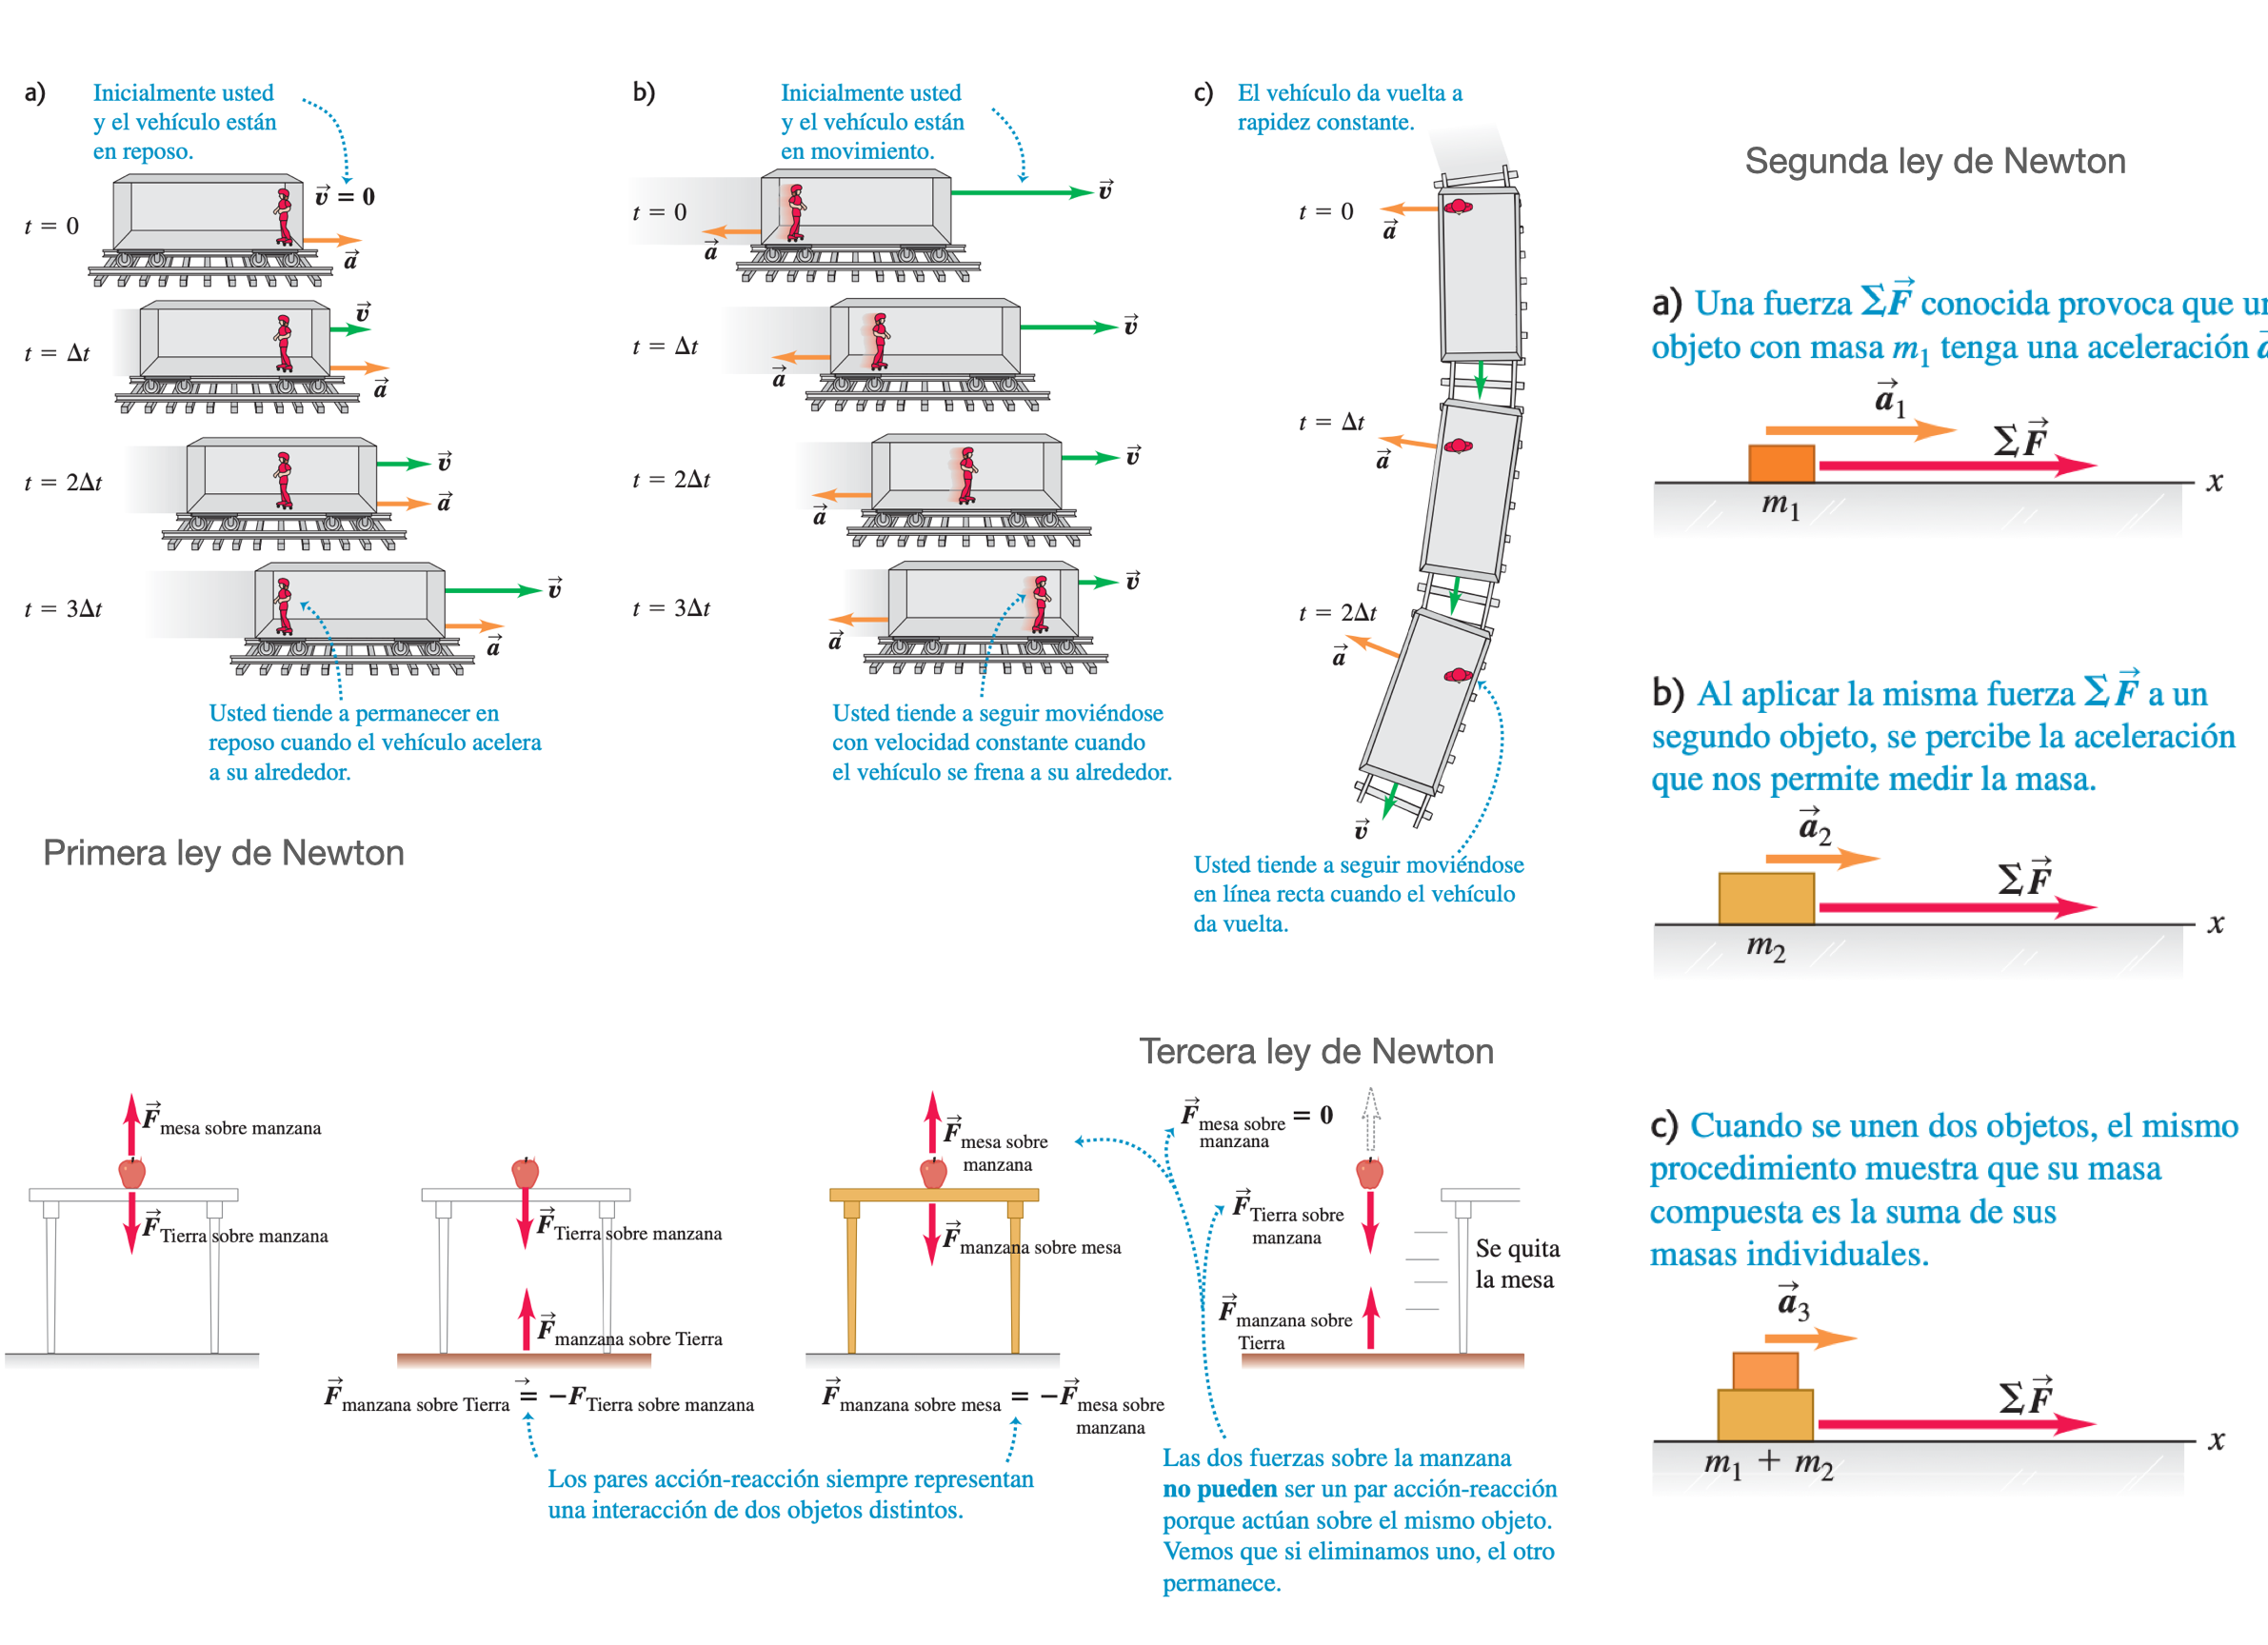
\includegraphics[width=1\textwidth]{imagenes/imagenes03/T03IM02.png}
		\end{figure}

Por extensión de la ley de Newton, tenemos: $Peso=m_G\; a \;\; \wedge\;\; F=m_I\; a$, donde $g$ es la aceleración de la gravedad, $m_G$ la masa gravitatoria y $m_I$ la masa inercial ($m$ es la constante de proporcionalidad entre $\vec F$ y $\vec a$).

\textbf{Igualdad entre masa inercial y masa gravitatoria: Otro enigma sin resolver.}

Fijémonos despacio en las fórmulas de Newton. Cuando aplicas una fuerza $\vec F$ a un cuerpo con cierta masa $m_I$, éste se acelera con cierta aceleración $\vec a\; / \vec F=m_I\; \vec a$. Hemos llamado $m_I$ a la masa para recordar que estamos hablando de la ``resistencia’’ que opone esa masa a acelerarse (su inercia; de ahí el subíndice `I’).

Pero sabemos que el mismo cuerpo ejerce una atracción gravitatoria sobre todos los demás. Por ejemplo, si pesamos ese cuerpo, lo que estamos haciendo es medir la fuerza gravitatoria entre él y la Tierra, que será $F=G \dfrac{M_T\; m_G}{{R_T}^2}$, donde $M_T$ es la masa de la Tierra, $R_T$ su radio y $m_G$ es la masa del cuerpo en cuestión (que ahora llamamos $m_G$ para remarcar que nos referimos a la masa que produce la atracción gravitatoria). 

Si ahora imaginamos un experimento fácil en el que queremos medir la aceleración que produce la fuerza de la gravedad, no tenemos más que igualar las dos fórmulas:
$$m_I\;a= G \dfrac{M_T\; m_G}{{R_T}^2} \to a= \dfrac{m_G}{m_I}\;G\dfrac{M_R}{{R_T}^2}$$
Midiendo la aceleración $a$ en muchos experimentos diferentes, con objetos de masas diferentes, se ve que es siempre igual (y por eso se le llama $g$, la aceleración de la gravedad en la superficie terrestre) y, por tanto,  $\boldsymbol {m_G/m_I=1}$, o sea encontramos que la masa gravitatoria es igual a la masa inercial en cualquier cuerpo. (Experimentos de EOTVOS-1891 y DICKE-1950)

La pregunta que ya se hizo Newton es: ?`por qué tienen que ser necesariamente iguales $m_I$ y $m_G$? Son conceptualmente diferentes: $m_I$ representa cómo una cantidad de materia se opone a que la aceleren mientras que $m_G$ representa cómo atrae esa cantidad de materia a cualquier otra.

Como hemos dicho, experimentalmente se mide que ambas son iguales. Pero tenemos que recordar que la precisión de los aparatos con los que medimos en los experimentos científicos no es infinita. Por tanto, no podemos estar absolutamente seguros de que sean exactamente iguales, lo más que podemos decir es que son iguales hasta una precisión muy elevada (una parte en diez billones). O sea, en una masa de un kilo, $m_I$ y $m_G$ podrían ser diferentes en una milmillonésima de miligramo, no más. Hecha esta aclaración, podemos asegurar que la masa inercial y la masa gravitatoria son iguales hasta donde alcanza la precisión de nuestras medidas.

Einstein también pensó en este enigma. No lo resolvió (es decir, no encontró una teoría que demostrara que las masas gravitacional e inercial tienen que ser iguales) pero, como estaba convencido de que dicha igualdad no era por casualidad, supuso que era un principio fundamental del universo (como el del límite de la velocidad de la luz) y lo llamo \textbf{\emph{``principio de equivalencia''}}. Este principio es fundamental en su teoría de la gravitación, la teoría general de la relatividad.

		
\section[Fuerzas de rozamiento, estático y dinámico]{Fuerzas de rozamiento, estático y dinámico \sectionmark{Fuerzas de rozamiento}}
\sectionmark{Fuerzas de rozamiento}

Al arrojar un cuerpo sobre una mesa observamos que	éste se desliza por ella y, al cabo de un tiempo	 $t$, se para. \emph{Las fuerzas de rozamiento son aquellas que actúan siempre oponiéndose al sentido del movimiento de los cuerpos.}

En un momento determinado en que hay un determinado número de pesas en la balanza, el cuerpo se pone en movimiento: $\ \boldsymbol{F\ge F_{RE}}$.

\begin{multicols}{2}

La fuerza de rozamiento estático depende de la naturaleza de los cuerpos que rozan.

La relación entre la fuerza máxima de rozamiento estático y la fuerza normal $(N)$ se llama \emph{coeficiente de rozamiento estático:} $\ F_{RE}=\mu_{RE}\ N$

En general,

$\vec F_{tot}=\vec F-\vec F_{RE}=m\ \vec a$

\begin{figure}[H]
		\centering
		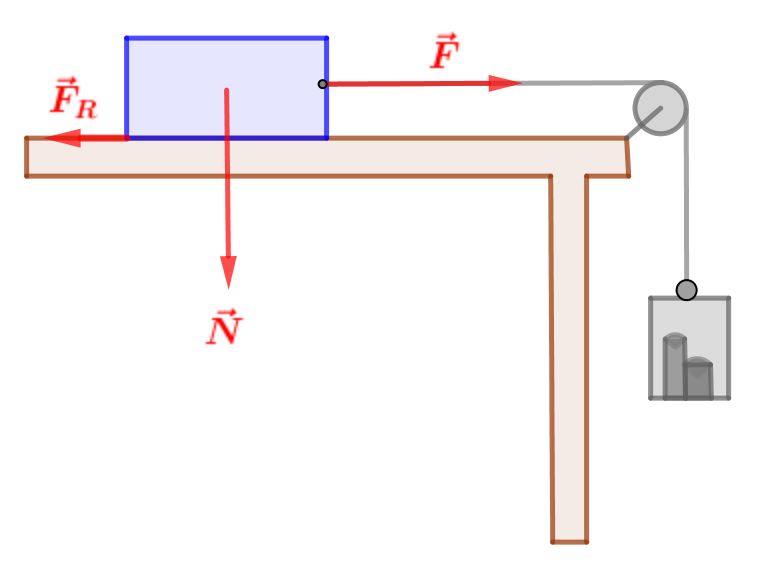
\includegraphics[width=.3\textwidth]{imagenes/imagenes03/T03IM48.png}
		\end{figure}		
\end{multicols}		
		
\textbf{Plano inclinado}
		
\begin{multicols}{2}
A medida que aumenta $\alpha$, aumenta la componente tangencial del peso, $\vec F_T$. En el momento en que el cuerpo empiece a deslizar,

$F_T=F_{RE}=\mu_{RE}\vec N \quad \to \quad \mu_E=\dfrac {m g \sin \alpha}{m g \cos \alpha}=\tan \alpha$
\begin{figure}[H]
		\centering
		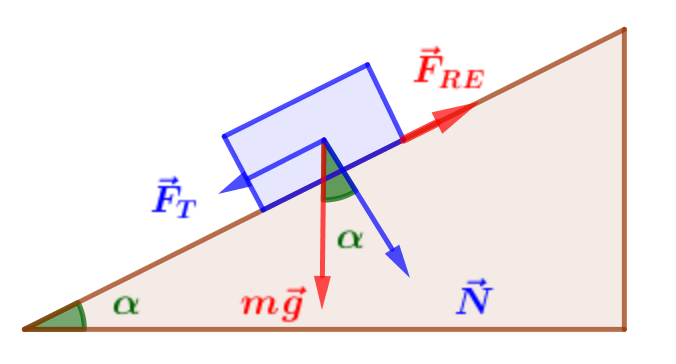
\includegraphics[width=.3\textwidth]{imagenes/imagenes03/T03IM49.png}
		\end{figure}		
\end{multicols}			
		

El coeficiente de rozamiento estático se puede encontrar como la tangente del ángulo mínimo para el que el cuerpo empieza a deslizar por el plano inclinado.

Experimentalmente se comprueba que, una vez empieza el cuerpo a moverse, la fuerza de mantenimiento puede ser menor que $F_{RE}$. Se suele hablar de \emph{rozamiento dinámico.}

$F_{RE}=\mu_{RE}\ N; \quad F_{RD}=\mu_{RD}\ N \le F_{RE} \Rightarrow \boldsymbol{\mu_{RD} \le \mu_{RE}}$		
		
$F_{RD}$ es la fuerza que hay que aplicar para mantener el cuerpo en movimiento.			


\begin{figure}[H]
		\centering
		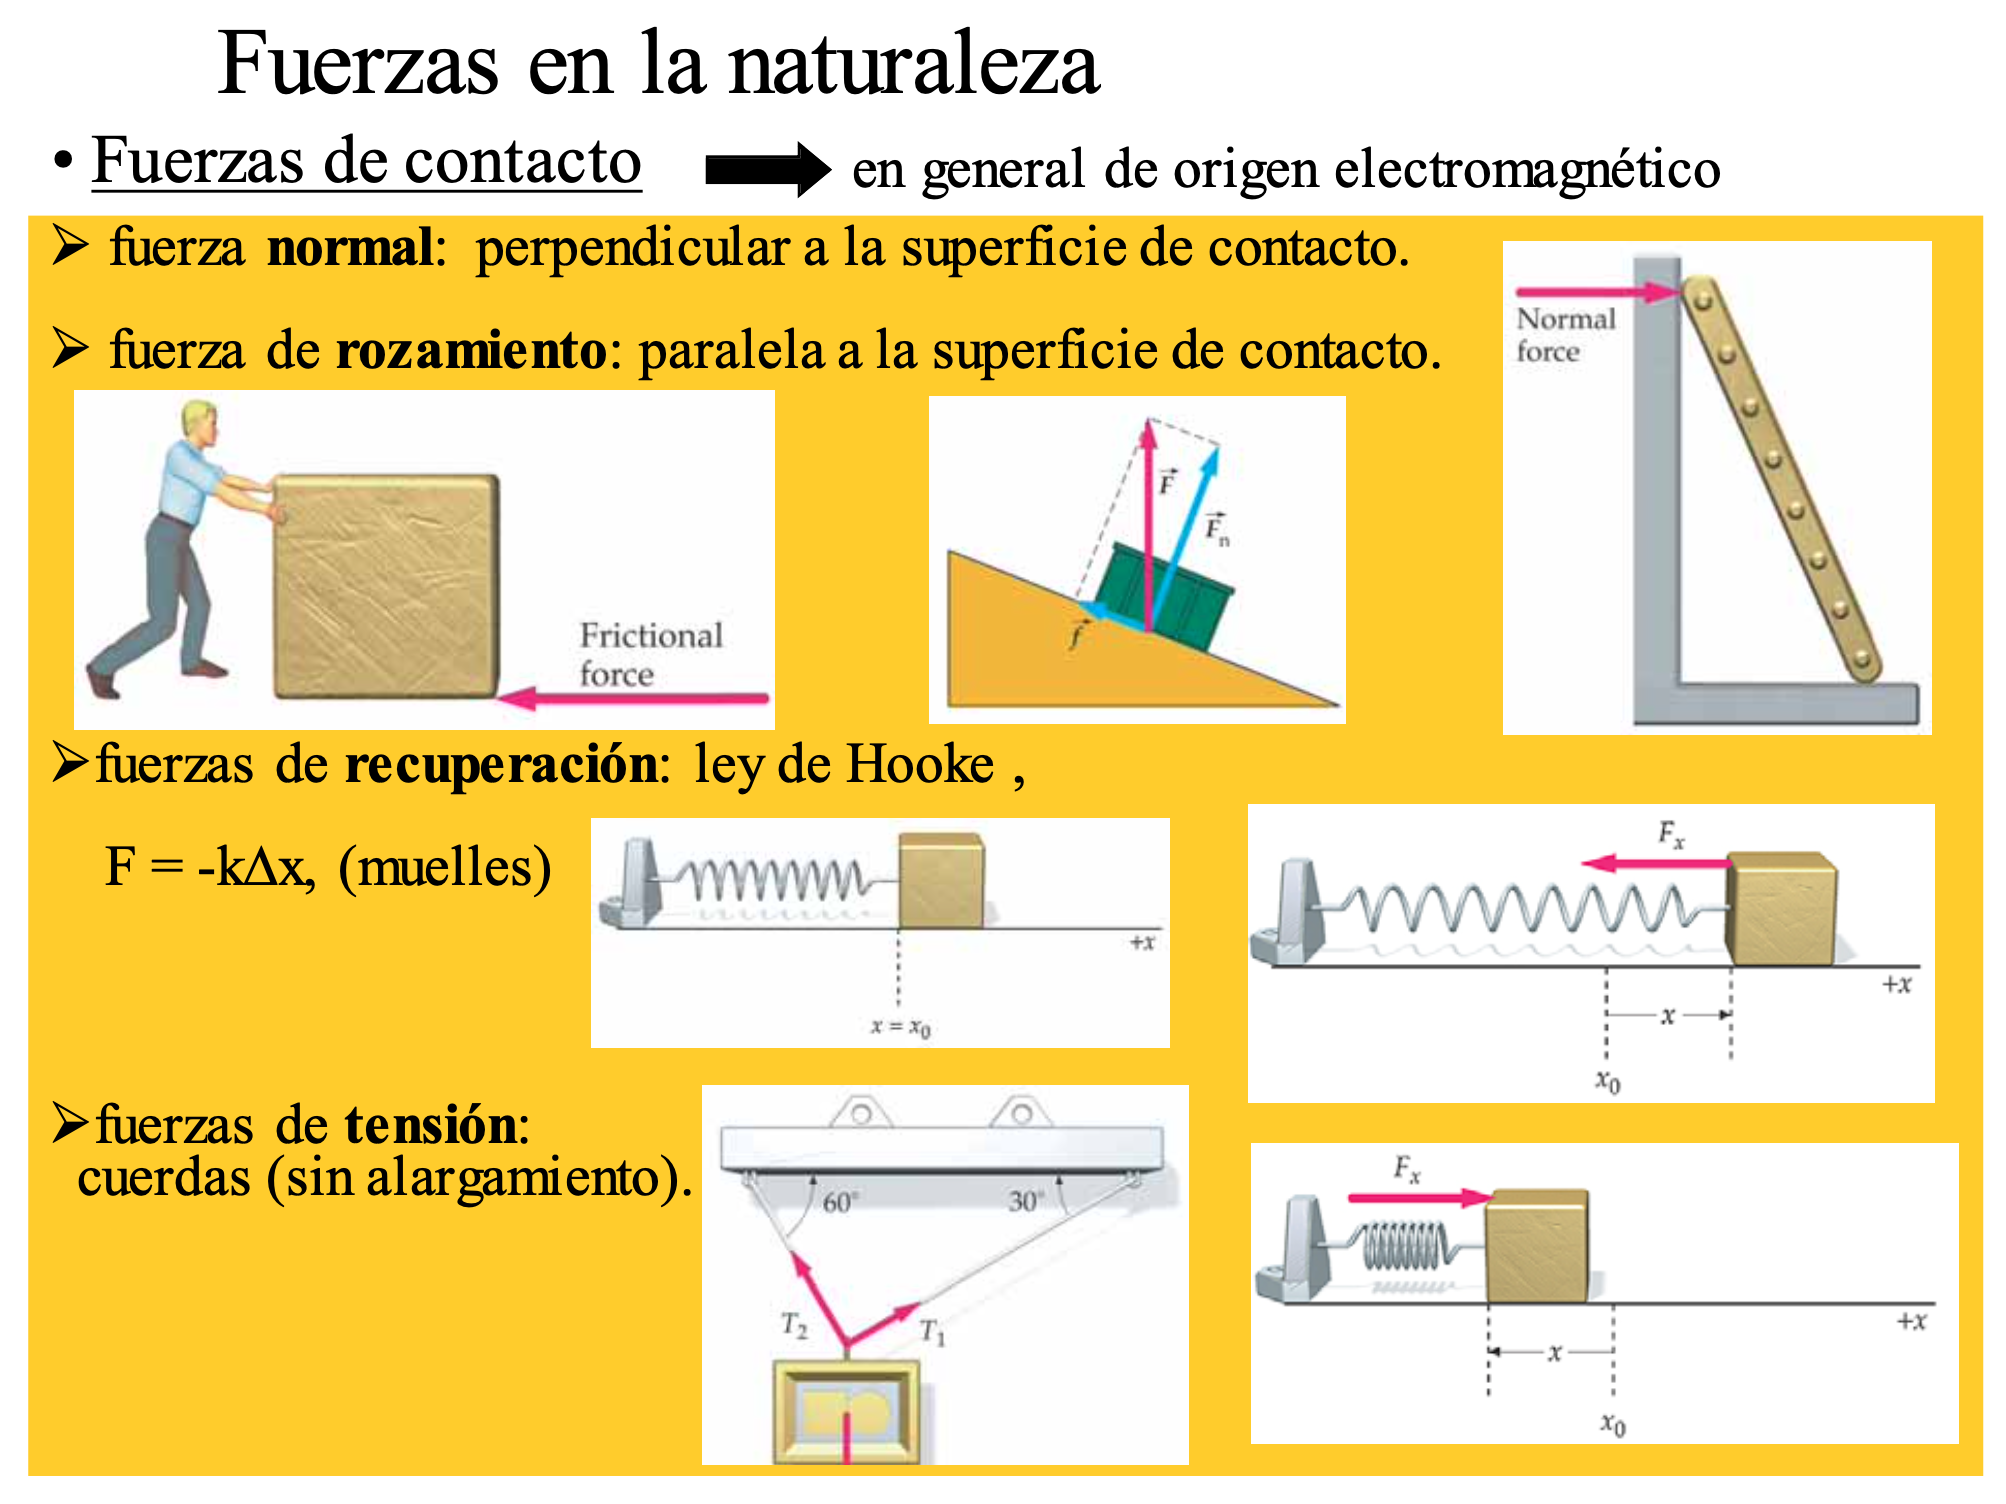
\includegraphics[width=.75\textwidth]{imagenes/imagenes03/T03IM06.png}
		\end{figure}
		
\vspace{10mm} %**********************************************
		
\begin{figure}[H]
		\centering
		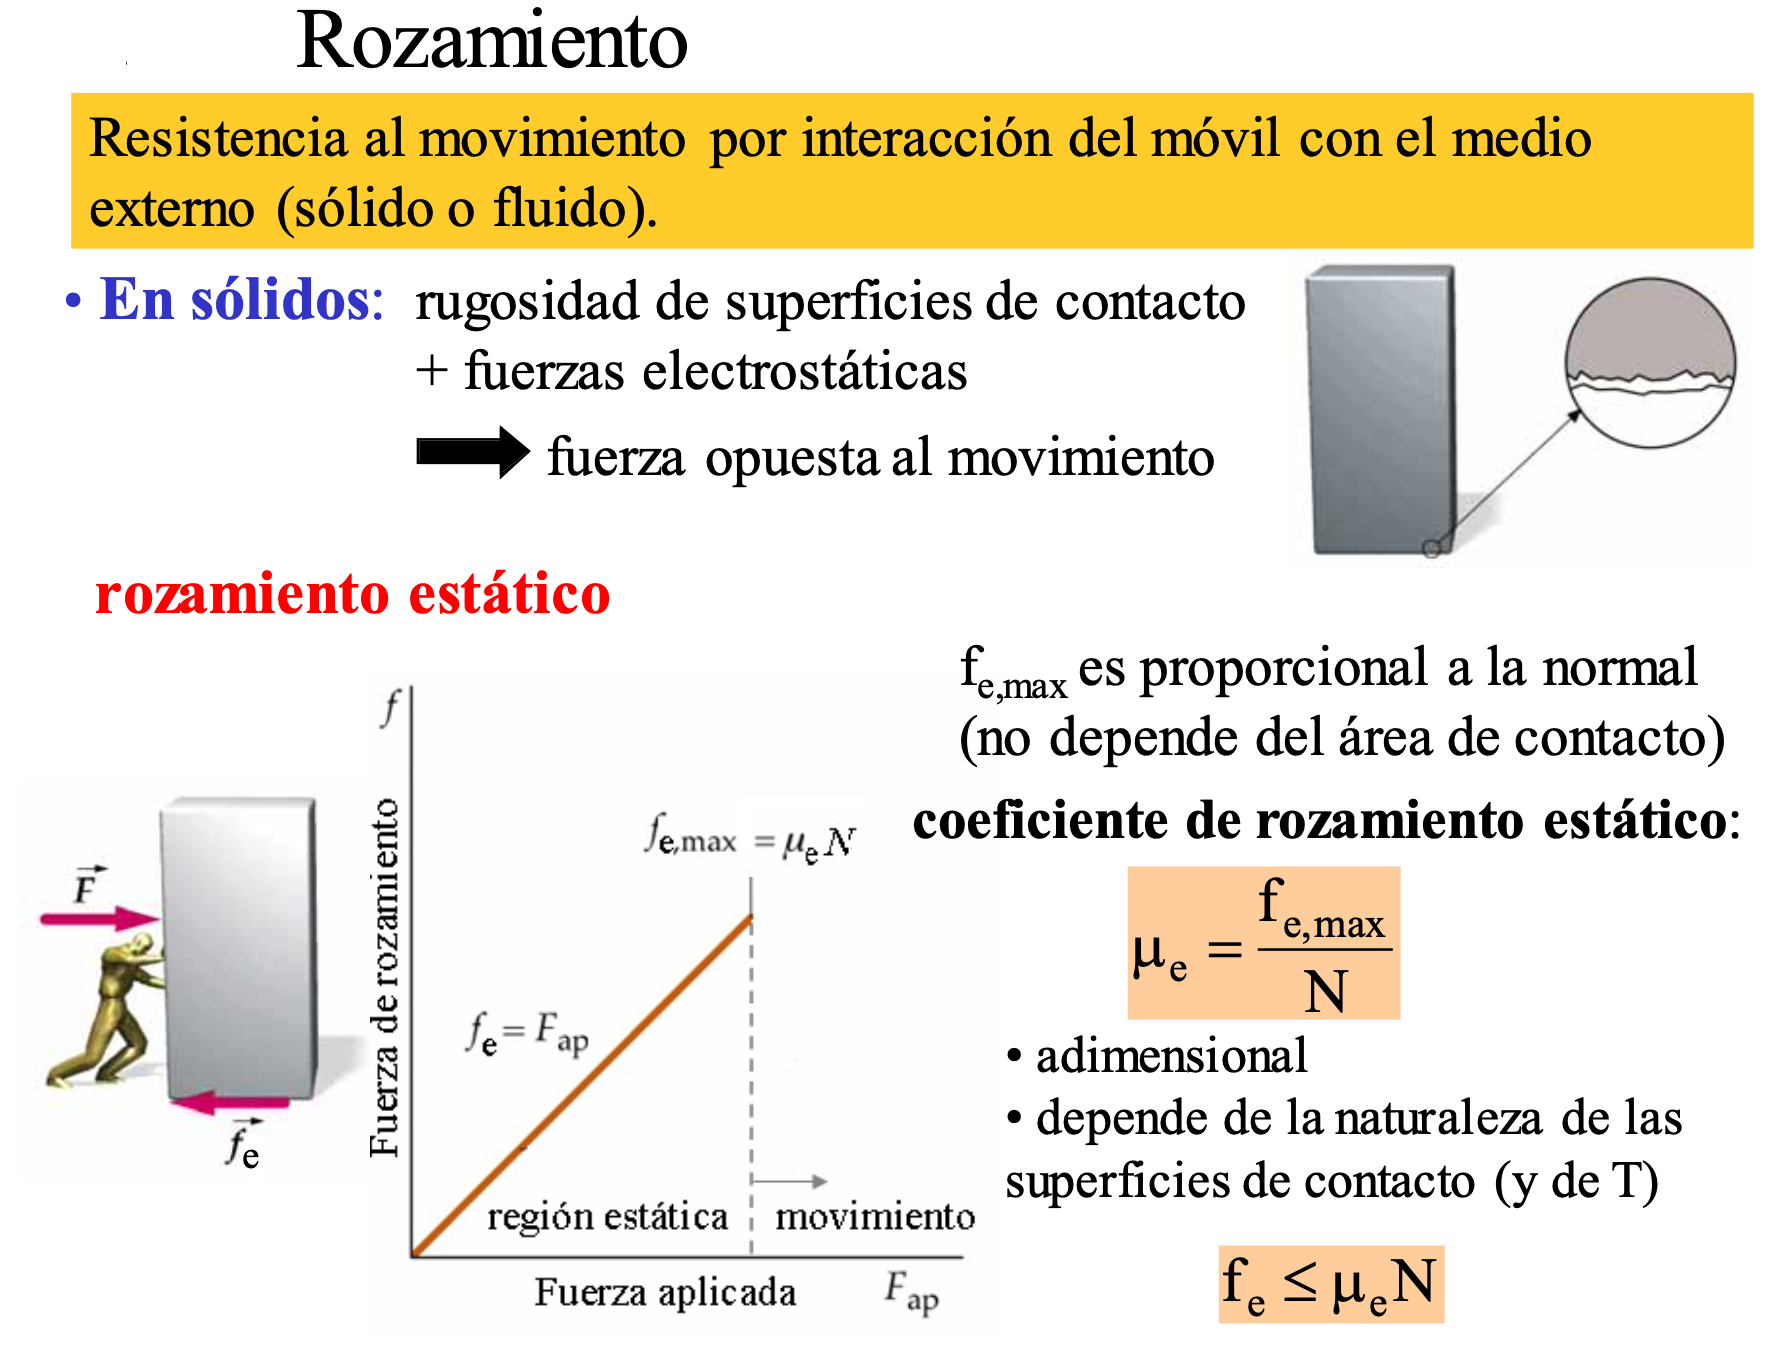
\includegraphics[width=1\textwidth]{imagenes/imagenes03/T03IM07.png}
		\end{figure}
		
		
\begin{figure}[H]
		\centering
		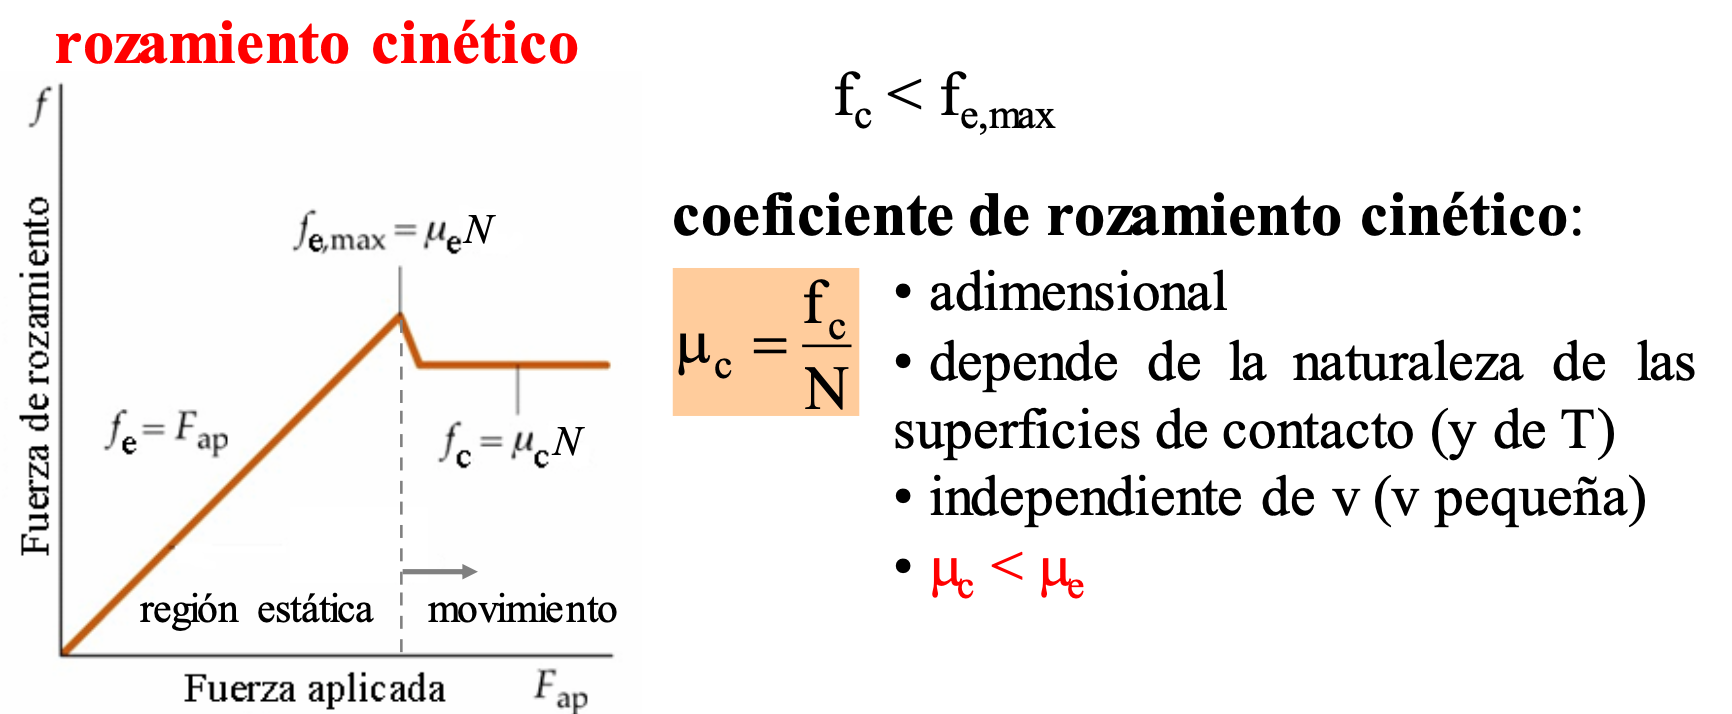
\includegraphics[width=1\textwidth]{imagenes/imagenes03/T03IM08.png}
		\end{figure}		

\newpage %*****************************************************

\begin{figure}[H]
		\centering
		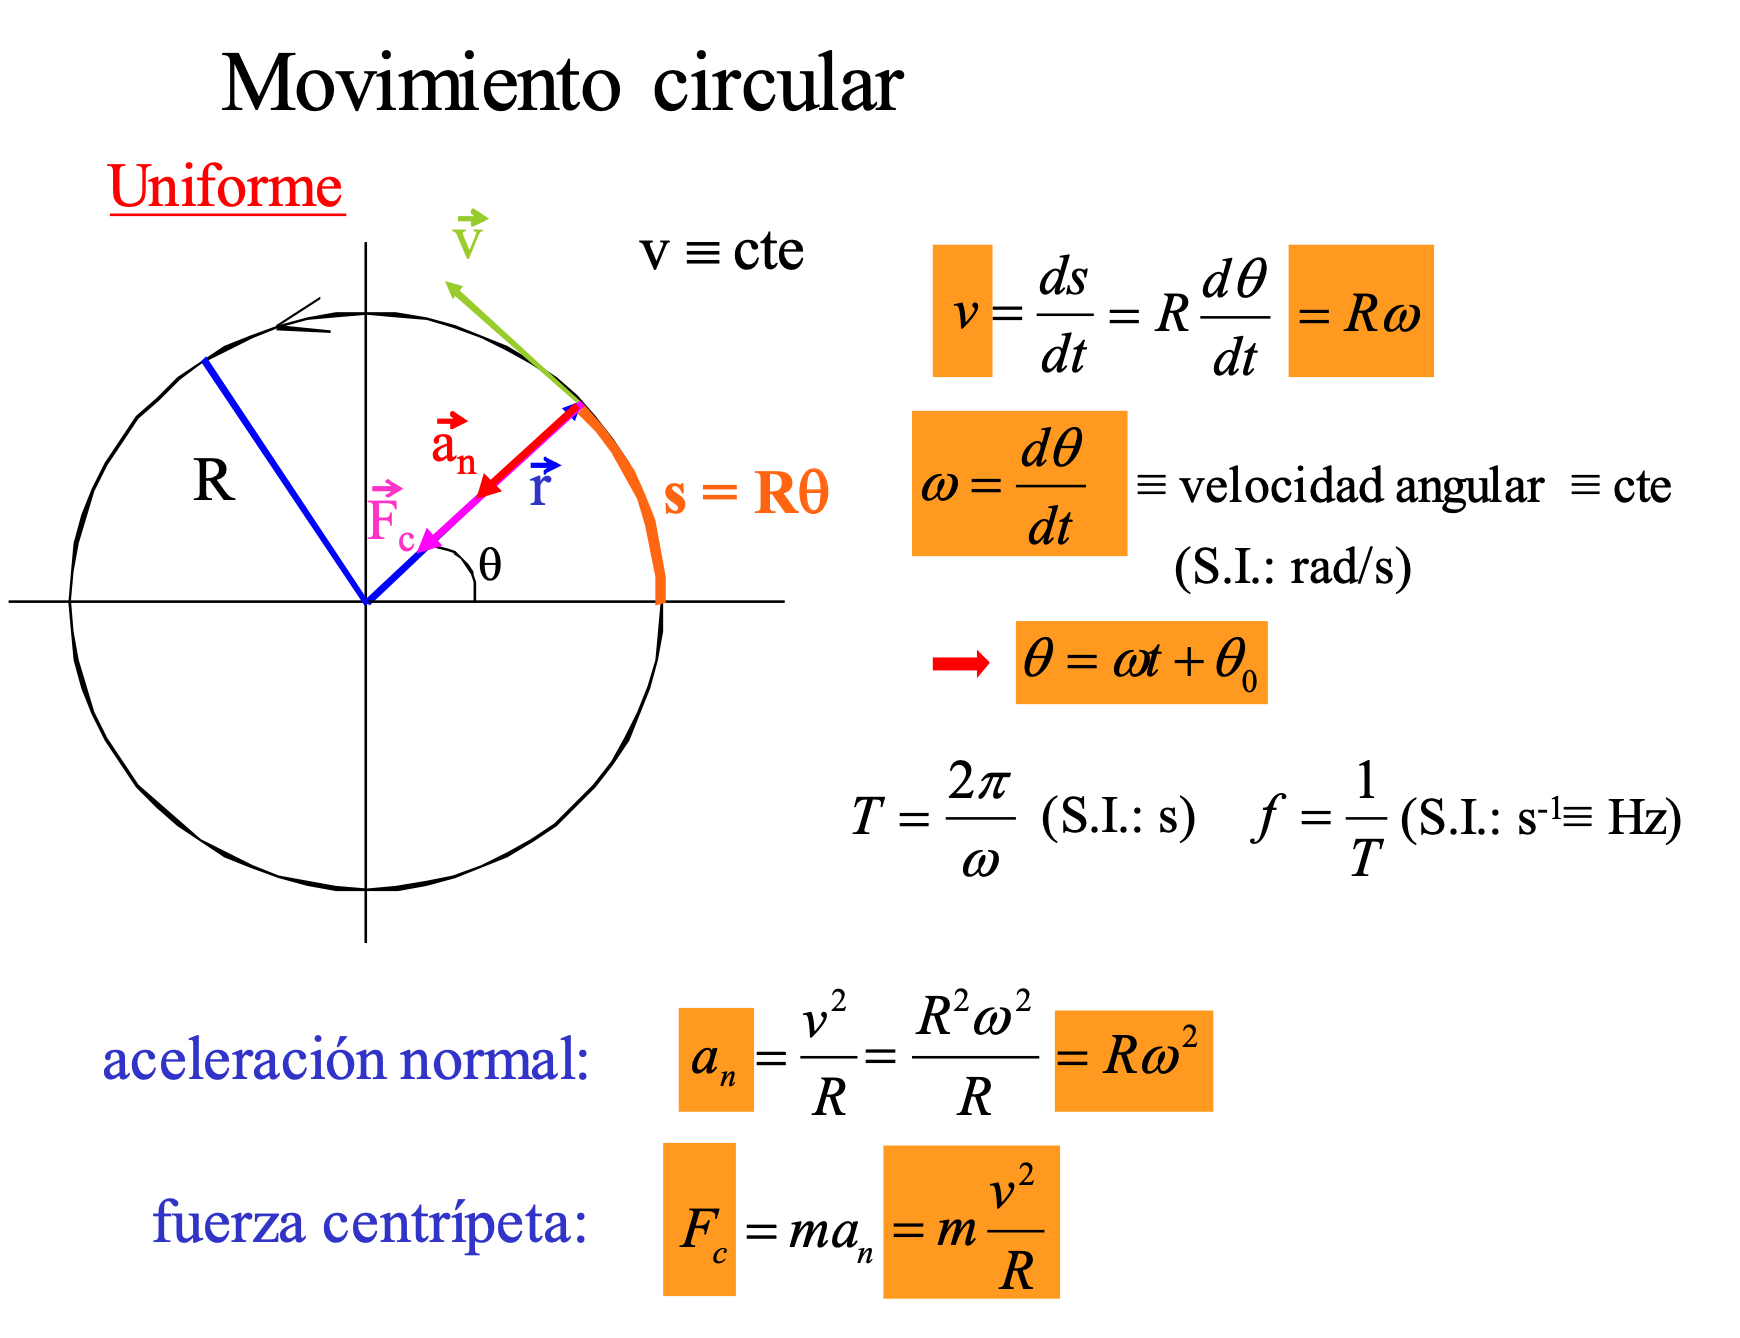
\includegraphics[width=.95\textwidth]{imagenes/imagenes02/T02IM31.png}
		\end{figure}

\begin{figure}[H]
		\centering
		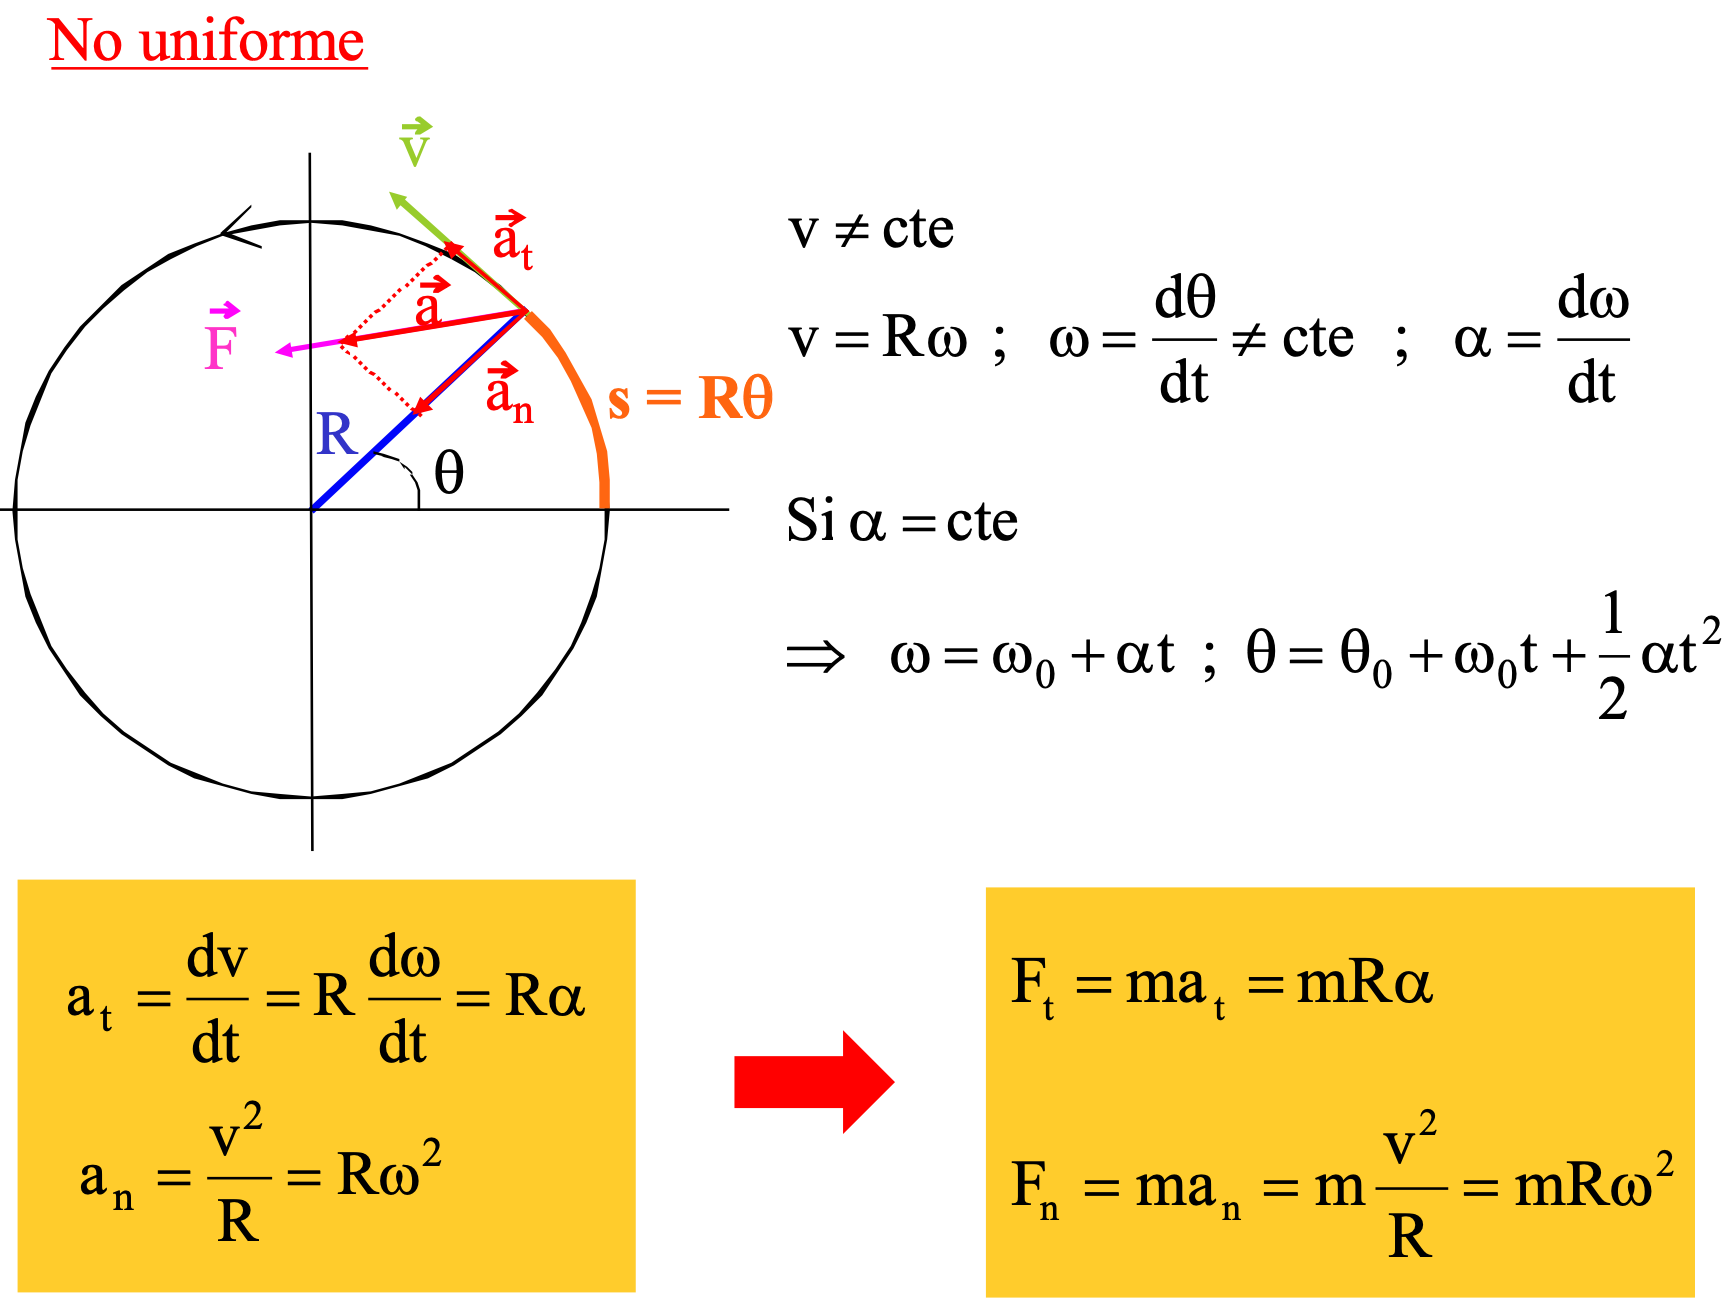
\includegraphics[width=.95\textwidth]{imagenes/imagenes02/T02IM32.png}
		\end{figure}

			
\section{Trabajo de una fuerza}

\begin{multicols}{2}
Por definición, diremos que el \emph{trabajo elemental} $\boldsymbol{\dd W}$ que realiza un cuerpo $m$  al pasar de una posición $\vec r$ a otra infinitamente próxima $\vec r+ \dd \vec r$ es: 

\begin{equation}
\label{def-trabajo}
\subrayado{\dd W= \vec F \cdot \dd \vec r}
\end{equation}

$ (\ \boldsymbol{\cdot} \ \equiv \text{producto\; escalar})$

\begin{figure}[H]
		\centering
		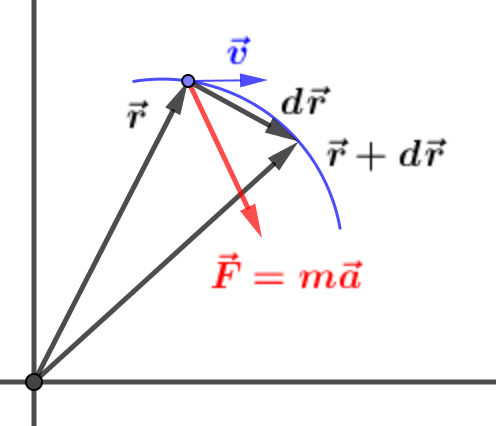
\includegraphics[width=.45\textwidth]{imagenes/imagenes03/T03IM01.png}
		\end{figure}
\end{multicols} 



El trabajo total para ir de un punto $A$ hasta otro $B$ es:

\begin{equation}
\label{trabajo}
W=\int_A^B\vec F \cdot \dd \vec r	
\end{equation}

En el caso particular en que $\vec F=\overrightarrow{cte}$, 
$W=\vec F \cdot \int_A^B \dd \vec r=\vec F\cdot (\vec r_B-\vec r_A)=\vec F \cdot \Delta \vec r$

\begin{multicols}{2}
Si además el desplazamiento es en línea recta, el trabajo es el producto del desplazamiento por la componente tangencial de la fuerza.º

\vspace{3mm} %**********************************************
$W=\vec F\cdot \Delta \vec r=F\; \Delta r\; 	\cos \theta= (F\; \cos \theta)\; \Delta r= F_T \;\Delta r$

\vspace{3mm} %**********************************************
Dimensionalmente, $[W]=[\mathrm{FL}]=[\mathrm{ML}^2\mathrm{T}^{-2}]$. Su unidad es el Joule, $\mathrm{J}=\mathrm{N} \cdot \mathrm{m}$. El trabajo es un escalar.
\begin{figure}[H]
		\centering
		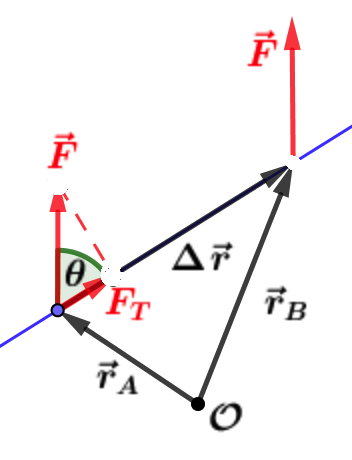
\includegraphics[width=.4\textwidth]{imagenes/imagenes03/T03IM03.png}
		\end{figure}	
\end{multicols}





\begin{figure}[H]
		\centering
		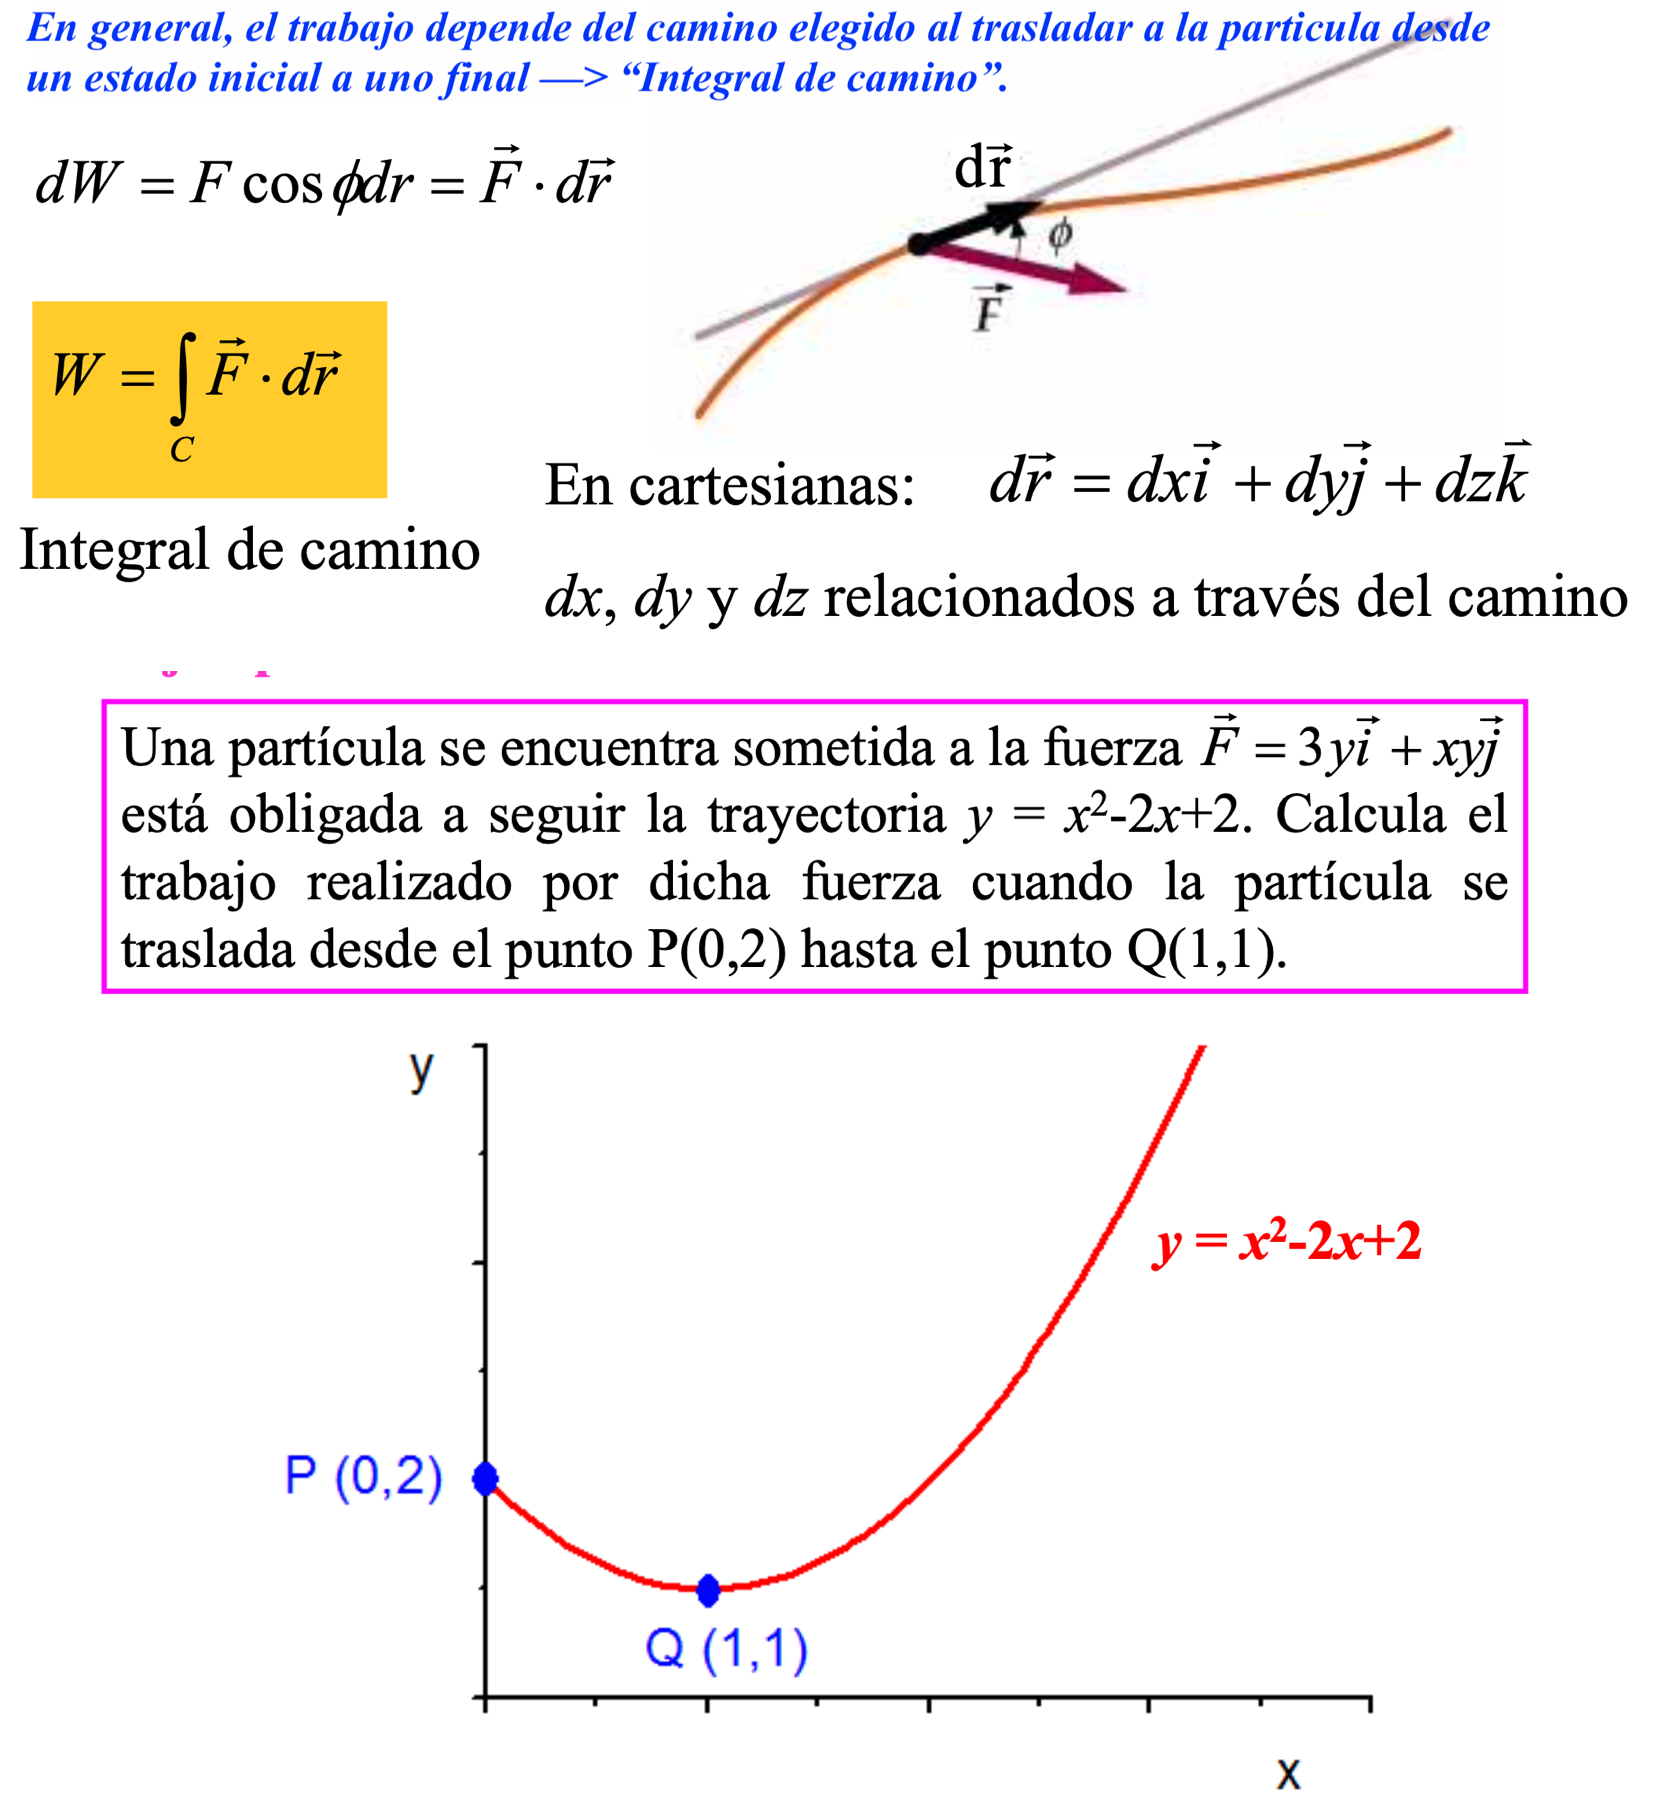
\includegraphics[width=.8\textwidth]{imagenes/imagenes03/T03IM04.png}
		\end{figure}

\vspace{-4mm}\noindent \small{\textcolor{gris}{$dW=\vec F \cdot \dd \vec r:\begin{cases}  \vec r=x\vec i +y \vec j \\  \vec F=\vec F(x,y) \end{cases} \hspace{-2mm}\to  y=y(x) \Rightarrow  \begin{cases} \dd \vec r=\dd \vec r(x,y(x)) \\ \vec F=\vec F(x) \end{cases} \hspace{-2mm} \dd W= \dd W(x)$}\normalsize{.}}

\begin{figure}[H]
		\centering
		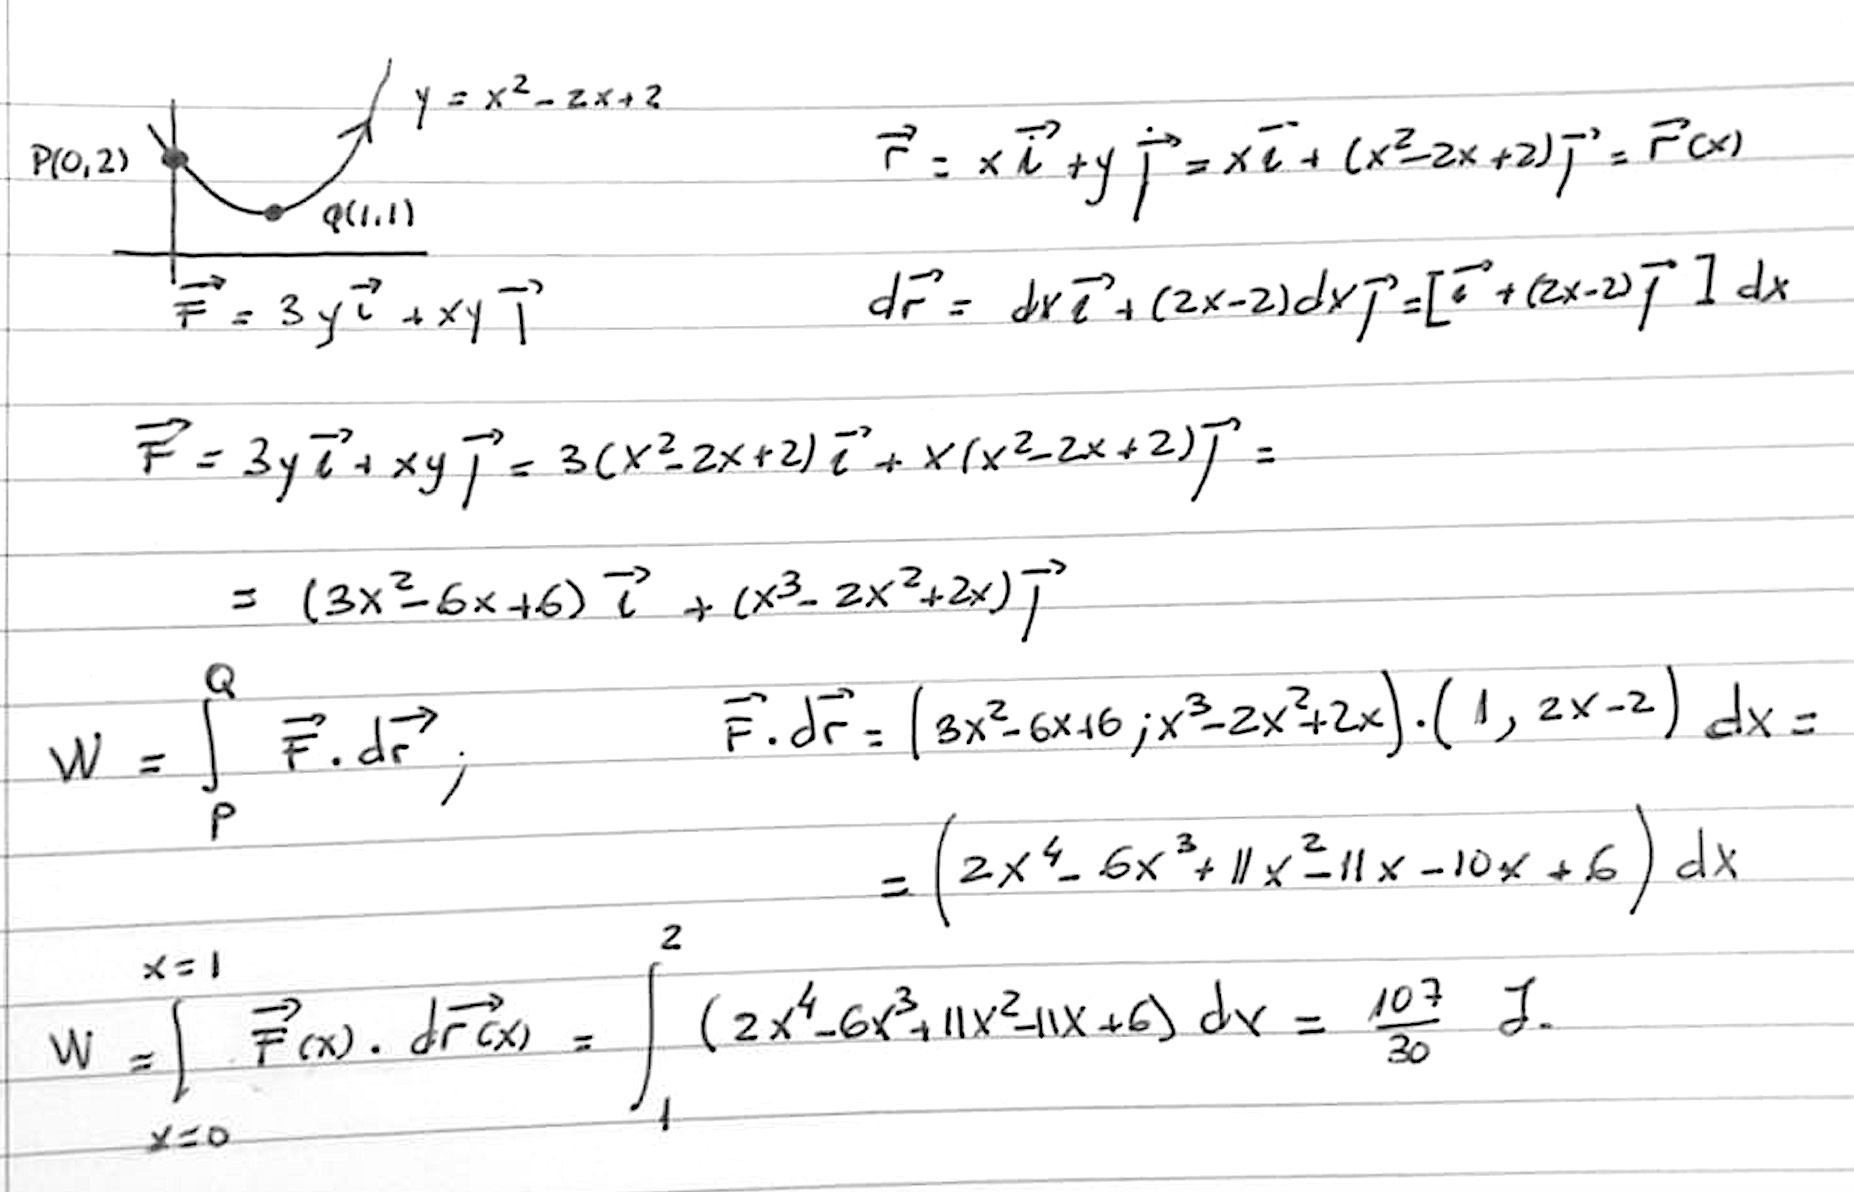
\includegraphics[width=.8\textwidth]{imagenes/imagenes03/T03IM13.png}
		\end{figure}

\section{Concepto de energía}

\normalsize{Un} \emph{fenómeno físico} es una variación en las condiciones que se dan en un sistema físico.

Podemos distinguir entre dos tipos de fueras:

\vspace{-2mm}\begin{itemize}
\vspace{-2mm}\item \emph{fuerzas exteriores} que actúan sobre un sistema físico y pueden modificarlo (al soltar un objeto de la mano cae al suelo por efecto de la fuerza externa de la gravedad que actúa sobre él).
\vspace{-2mm}\item \emph{fuerzas interiores} que actúan sobre un sistema físico y pueden modificarlo 	(un átomo de carbono 14 se convierte en nitrógeno 14 emitiendo un electrón --- desintegración $\beta:\; ^{14}_6C \to ^{14}_7N+^0_{-1}e$---).
\end{itemize}

Cuando se modifica el estado de un sistema físico se atribuye a las fuerzas y producen movimientos. \emph{Las fuerzas en movimiento son trabajo}, luego los sistemas físicos tienen \emph{energía}. 

Llamamos \emph{\colorbox{LightYellow}{energía}} a \emph{la \colorbox{LightYellow}{capacidad} que tienen los sistemas físicos para \colorbox{LightYellow}{realizar un trabajo}.}, es una propiedad que tienen los cuerpos y se va a medir con las mismas unidades y dimensiones que el trabajo. La energía es un escalar.

Podemos distinguir entre tres tipos de energia:

\begin{miparrafo}

\textbf{---} \emph{Energía cinética}: capacidad para realizar trabajo que tiene un cuerpo debido a su estado de movimiento (proyectil estrellado contra una pared).

\textbf{---} \emph{Energía potencial}: capacidad para realizar trabajo que tiene un cuerpo debido a la posición que ocupa en el espacio  (objeto que cae desde una determinada altura)

\textbf{---} \emph{Energía interna}: capacidad para realizar trabajo que tiene un cuerpo debido a su propia estructura interna (petardo de pólvora que explota por la temperatura).

\end{miparrafo}

La cantidad total de energía que tiene un sistema físico no es medible por la mecánica clásica, solo podemos medir variaciones de energía.


\section[Energía cinética. Teorema de las fuerzas vivas]{Energía cinética. Teorema de las fuerzas vivas\sectionmark{Energía cinética}}
\sectionmark{Energía cinética}

Definimos la energía cinética $\;\mathcal E_c\;$ como el trabajo necesario para que un cuerpo de masa $m$ cambie su celeridad (módulo de la velocidad) desde $v_0$ a $v_f$.
$$\subrayado{\Delta \mathcal E_c=W}=\displaystyle \int_1^2 \vec F \cdot \dd \vec r$$
desde el estado $1\to v_o$ hasta el estado $2\to v_f$. Por la segunda de Newton:

$\Delta \mathcal E_c=\displaystyle \int_1^2 \dv{\vec p}{t}\cdot \dd \vec r =\int_1^2 \dd \vec p \cdot \dv{\vec r}{t}
= \int_1^2 \vec v \cdot \dd \vec p=\dfrac 1 m\int_1^2 m\;\vec v \cdot \dd \vec p=
\dfrac 1 m \int_1^2 \vec p\cdot \dd \vec p$

$p^2=\vec p\cdot \vec p \to $ tomando diferenciales: $\cancel{2\;} p\;\dd  p= \cancel{2}\; \vec p \cdot \dd \vec p \to\;\; p\;\dd p=\vec p \cdot \dd \vec p$

$\Delta \mathcal E_c=\displaystyle \int_1^2 \dfrac 1 m \;p\; dp=\int_1^2 v\;\dd p =\int_1^2\; v  \dd (mv)=\int_1^2 m (m\dd v + v\dd m)$

\begin{equation}
	\Delta \mathcal E_c=\displaystyle\int_1^2 m\ v\;\dd v + \int_1^2 v^2 \ \dd m
\end{equation}

Ecuación que da la expresión exacta de la energía cinética entre deos estados $1$ y $2$


En el caso especial de partículas o cuerpos rígido, $ m=cte  \to  \Delta \mathcal E_c= \displaystyle m\ \int_1^2 v \ \dd v $:

\begin{equation}
\label{fuerzas-vivas}
\Delta \mathcal E_c= \frac 1 2 \ m \ v_2^2 - \frac 1 2 \ m \ v_1^2 = \mathcal E_{c_2}-\mathcal E_{c_1}
\end{equation}

Ecuación que recibe el nombre de \emph{\colorbox{LightYellow}{`Teorema de las fuerzas vivas'}.}
(Leibniz, en el $s.\ XVII$ llamó ``fuerza viva'' al producto $m \ v^2$).

\emph{El trabajo realizado por las fuerzas del campo al evolucionar el sistema dede un estado $1$ con $v_1$ a un estado $2$ con $v_2$ viene dado por la diferencia entre energías cinéticas ($\frac 1 2$ fuerza viva) entre el estado final $2$ y el estado inicial $1$.}


En el supuesto que:
\vspace{-2mm}\begin{itemize}
\vspace{-2mm}\item $v_1>v_2 \to \mathcal E_1 < \mathcal E_2 \to \Delta \mathcal E_c<0$ y el trabajo desarrollado se usa en frenar a la partícula.
\vspace{-2mm}\item $v_1<v_2 \to \mathcal E1 < \mathcal E_2 \to \Delta \mathcal E_c>0$ y el trabajo desarrollado se invierte en acelerar a la partícula.
\vspace{-2mm}\item $v_1=v_2 \to \mathcal E_1 = \mathcal E_2 \to \Delta \mathcal E_c=0$ y no se realiza trabajo. 	
\end{itemize}

\begin{figure}[H]
		\centering
		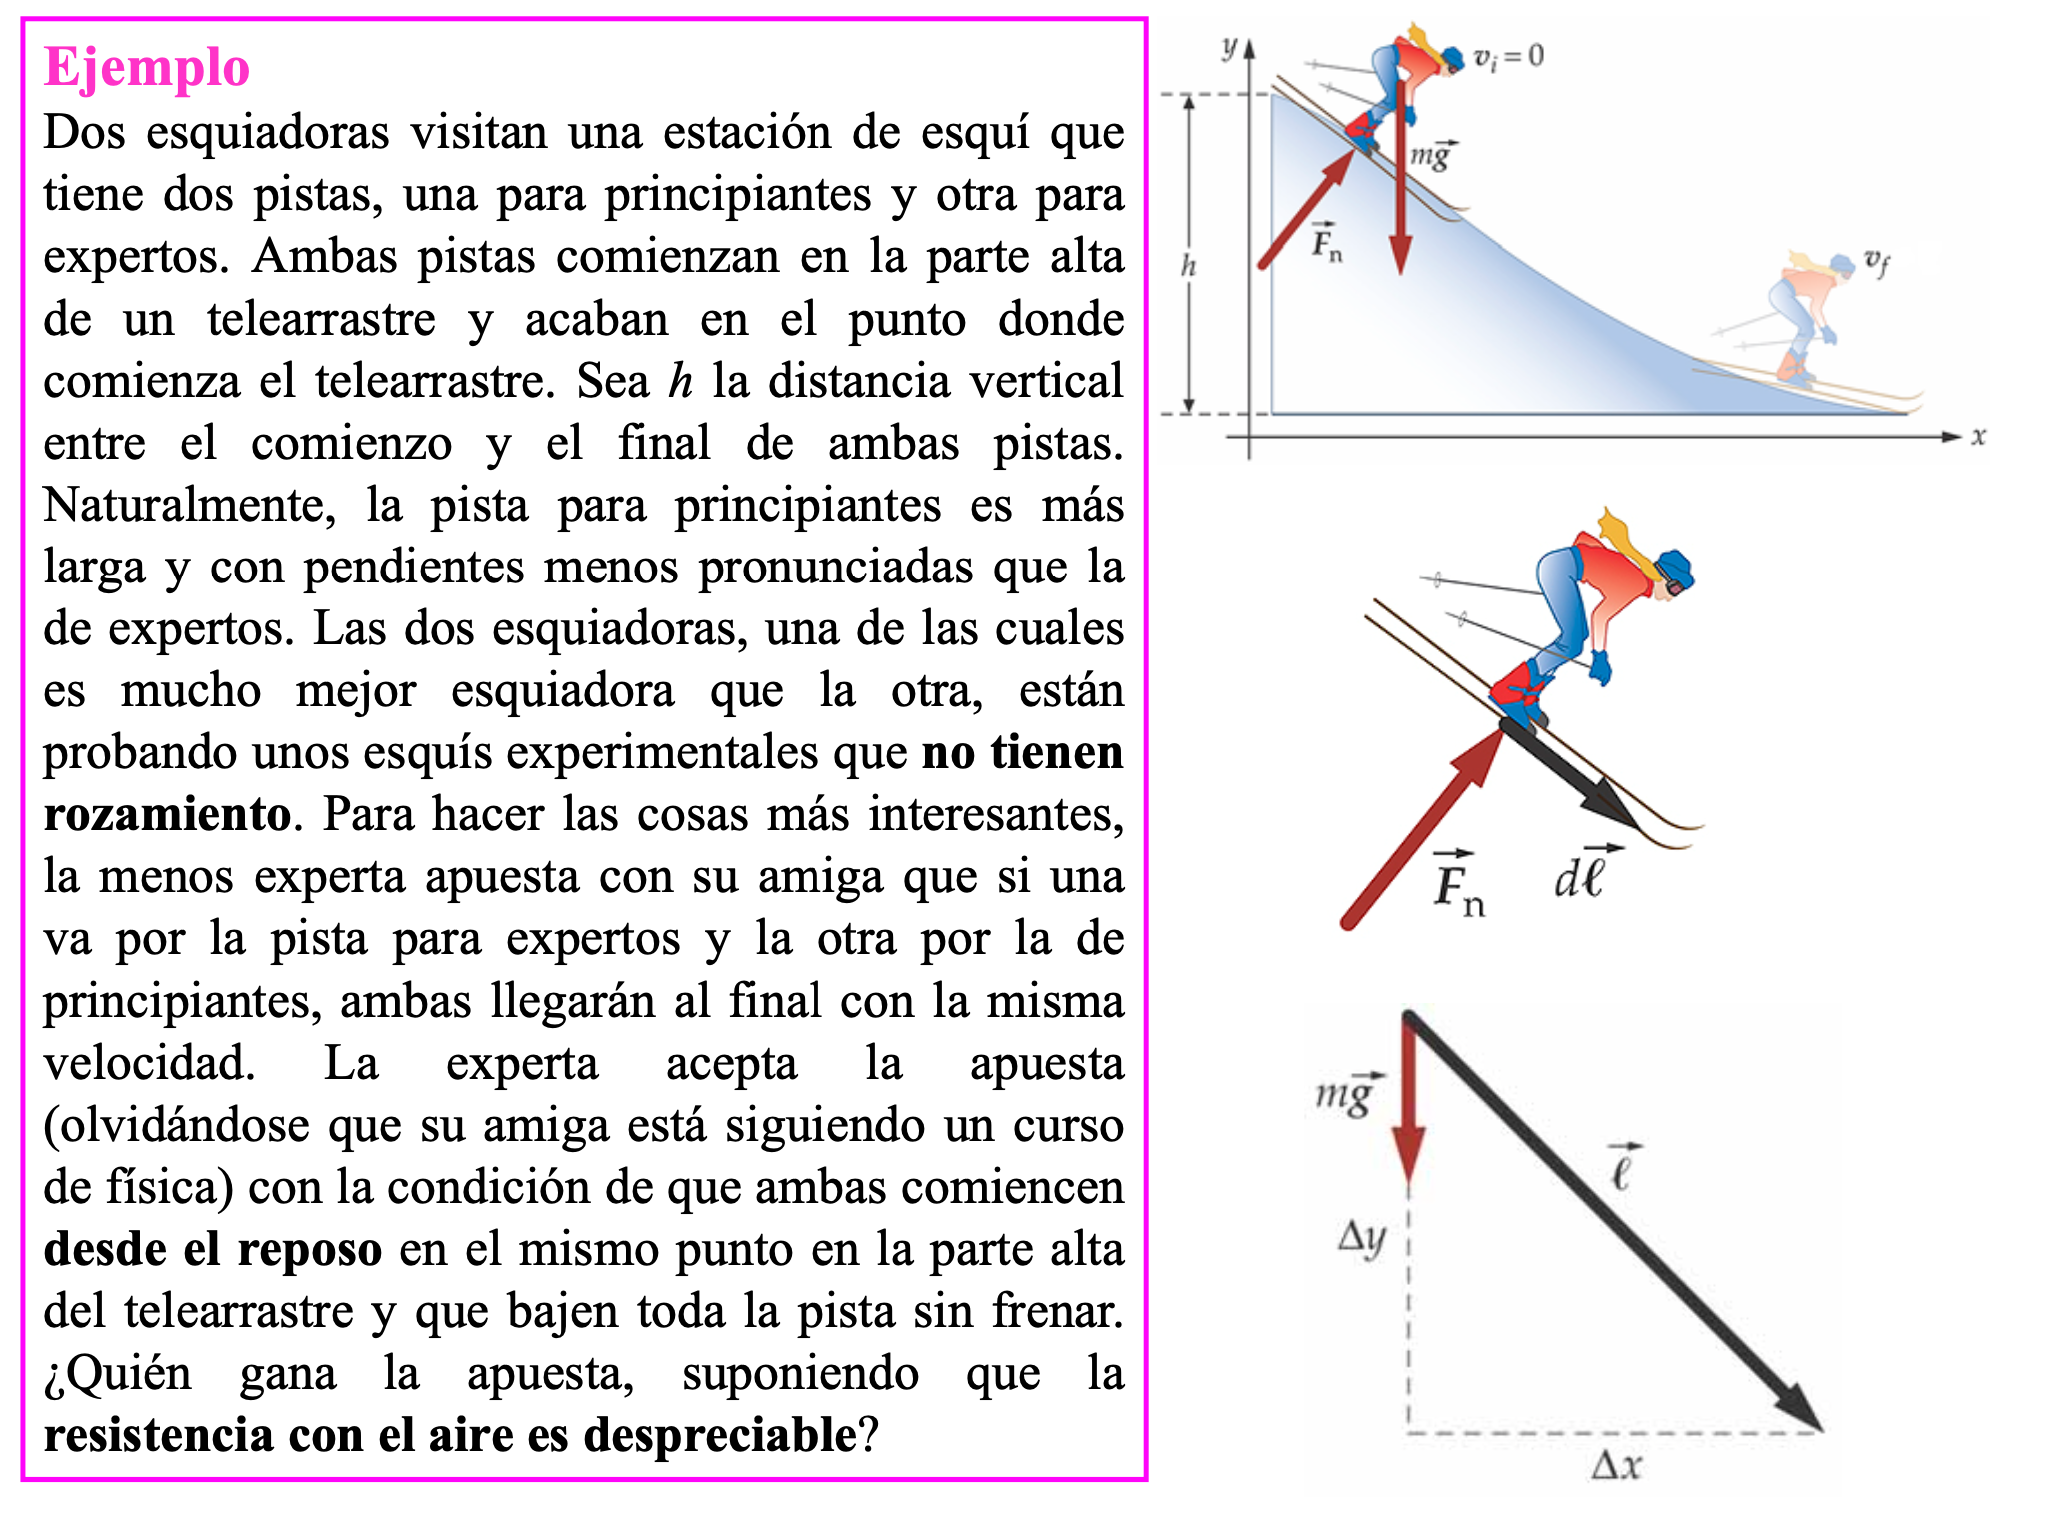
\includegraphics[width=1\textwidth]{imagenes/imagenes03/T03IM05.png}
		\end{figure}


\begin{multicols}{2}
	$W=\Delta \mathcal E_c==\frac 1 2 m v_f^2-\frac 1 2 m v_i^2$
	
	$\vec F=\vec N+\vec T$
	
	$\dd W _M=\vec N \cdot \dd \vec s=$
	
	$=(mg\sin \theta) \dd s \cos 90^o=0\to $ 
	
	$\to \quad W_N=0$
	\begin{figure}[H]
		\centering
		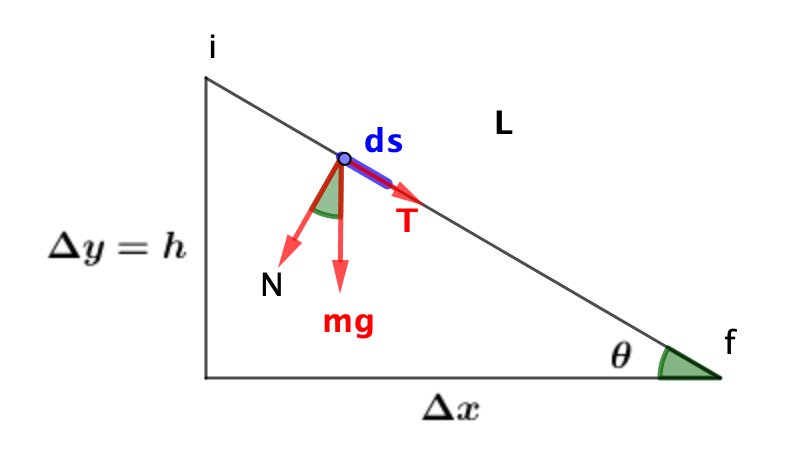
\includegraphics[width=.55\textwidth]{imagenes/imagenes03/T03IM47.png}
		\end{figure}
\end{multicols}
\vspace{-5mm}$\dd W_T= \vec T \cdot \dd \vec s=(mg \sin \theta) \dd s \cos 0^o \to W_T=mg\sin \theta \int_1^2 ds
=ms \sin \theta L=mgh$

$W=0+mgh=mgh=\mathcal E_c=\frac 1 2 m v_f^2$, parten del reposo: $v_i=0$

Luego $v_f=\sqrt{2gh}$. Ambas patinadoras llegan a meta con la misma velocidad y la menos experta gana la apuesta.

\textcolor{gris}{La patinadora que baja por la pista para expertos invierte menos tiempo en la bajada, pero esa no era la apuesta.}

\section{Potencia}

Se llama \emph{potencia} suministrada por una fuerza al trabajo por unidad de tiempo que realiza dicha fuerza. 

Potencia media: $\quad P=\dfrac{\Delta W}{\Delta t}$

Potencia instantánea: $\;\; P=\dfrac {\dd W}{\dd t}=\dfrac {\vec F \cdot \dd \vec r}{\dd t}=\vec F \cdot \vec v$

En general, para cualquier transferencia de energia, la potencia es: $\quad P=\dfrac{\dd E}{\dd t}$

Unidades: En el $SI:\;\; P\to  \ \mathrm{J s}^{-1} = \mathrm{W}$, wat. Una unidad de energía muy usada en ingeniería es el $\mathrm{kWh}=(10^3\ \mathrm{W})\ (3600\ \mathrm{s})=3.6\ 10^6 \ \mathrm{J}$.

\begin{ejem}
Un ascensor de $1000\ \mathrm{kg}$ soporta una carga máxima de $800 \ \mathrm{kg}$. Una fuerza de rozamiento constante de $400 \ \mathrm{N}$ retarda su movimiento hacia arriba haciendo que la subida sea a velocidad constante de $3 \ \mathrm{ms}^{-1}$. ?`Qué potencia suministra el motor?	
\end{ejem}
$F-F_R-(M+m)g=0 \to F=(1000+800)\ 9.8-4000=13640\ \mathrm{N}$

$P=F\ v=13640 \cdot 3 = 40920 \ \mathrm{W}= 40.920 \ \mathrm{KW}$

\textbf{Potencia y energía cinética.}

En una dimensió: $\displaystyle P=Fv=mav = m \dv{v}{t} v =\dv{t}(\dfrac 1 2 mv^2)\Rightarrow P=\dv{\mathcal E_c}{t}$.

Si $P=cte \to \quad P=\dfrac{\Delta \mathcal E_c}{\Delta t} $

\begin{ejem}
\normalsize{Un} móvil acelera desde el reposo hasta $100	\ \mathrm{ms}^{-1}$ en $10 \mathrm{s}$. Su masa es de $2\ \mathrm{Kg}$. Suponiendo que esta aceleración se alcance a potencia constante, ?`cuál es la potencia desarrollada por el motor? ?`Cuánto tiempo necesitará para, en las mismas condiciones, doblar su velocidad?
\end{ejem}

$P=\dfrac{\Delta \mathcal E_c}{\Delta t}=\dfrac{\frac 1 2 \ 2 \ 100^2 - 0}{10}=1000 \mathrm{W}$

$P=\dfrac{\Delta \mathcal E_c}{\Delta t} \to 1000=\dfrac{\frac 1 2 \ 2 \ 200^2 - \frac 1 \ 2 \ 2 100^2}{\Delta t} \to \quad \Delta t=30\ \mathrm{s}$


\section{Campos de fuerza}

En una determinada región del espacio existe un \emph{campo de fuerza} cuando por el hecho de situar en cualquier parte de esta región un cuerpo, \emph{instantáneamente} aparece sometido a una fuerza.

En `teoría clásica de campos' la interacción entre cuerpos del universo es \emph{instantánea}. La `teoría relativista de campos'  no permite la interacción instantánea, ninguna interacción se propaga a velocidad superior a la de la luz en el vacío, $c$. \footnote{Ver en Apéndice \ref{concepto-campo} el artículo ``Los conceptos de campo''.}

Llamamos \emph{magnitud activa de campo, $A$}, a la propiedad que tienen los cuerpos al interaccionar con los campos: $m$ en la interacción gravitatoria, $q$ en la eléctrica, .... Si $\vec E$ es la intensidad del campo en cuestión, $\vec F=A\ \vec E$.

\subsection{Campos conservativos. Campo central}

\begin{multicols}{2}
Propiedad de los campos de fuerza \textbf{conservativos}: \emph{``El \underline{trabajo} realizado por un campo de fuerza (conservativo) para que la magnitud activa del campo se desplace desde un punto $A$ hasta otro $B$ es \underline{independiente del camino recorrido}, depende solo de los instantes inicial y final.''}
\begin{figure}[H]
		\centering
		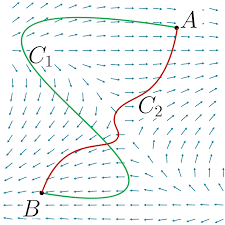
\includegraphics[width=.2\textwidth]{imagenes/imagenes03/T03IM09.png}
		\end{figure}
\end{multicols}

\begin{multicols}{2}
Un caso particular de campo conservativo muy importante es el \emph{campo central:} cuando se deposita una magnitud activa en el campo aparecen sobre ella las fuerzas del campo que están dirigidas hacia el \emph{centro de fuerzas} y suelen ser \emph{inversamente proporcionales al cuadrado de la distancia} de la posición que ocupa la magnitud activa al el centro de fuerzas.
\begin{figure}[H]
		\centering
		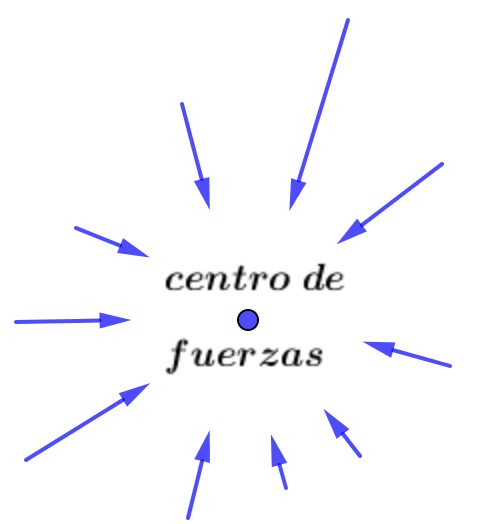
\includegraphics[width=.25\textwidth]{imagenes/imagenes03/T03IM10.png}
		\end{figure}
\end{multicols}

\emph{Un campo de fuerzas central es necesariamente conservativo.} Al ser central solo depende de la posición del centro de fuerzas y varía con la distancia (no necesariamente como $1/r^2$), veamos que es conservativo:

Sea $\mathcal A$, la magnitud activa del campo central $\vec E$,

$\Vec F=\mathcal A \; \vec E= \mathcal A \; \vec u_r \; \varphi(r)$, donde $\vec u_r=\dfrac {\vec r}{r}$ es un vector unitario que apunta al centro de fuerzas desde la posición que ocupe la magnitud activa y $\varphi(r)$ es la forma en que varía $\vec E$ con la distancia al centro de fuerzas.

 Calculemos el trabajo necesario para desplazar la magnitud activa $\mathcal A$ bajo la acción del campo central $\vec E$ desde un punto $A$ hasta otro $B$.
 
 $\displaystyle W=-\int_A^B \mathcal A\; \varphi(r) \;\vec u_r \cdot \dd r= -\int_A^B \mathcal A\; \varphi(r) \; \dfrac {\vec r}{r} \cdot \dd r =(*) -\int_A^B \mathcal A\; \varphi(r) \; \dfrac {\cancel{r}\;\dd r}{\cancel{r}}=-\int_A^B \mathcal A\; \varphi(r)\; \dd r=(**)-\eval{\Phi(r)}_{A}^B=-[\Phi(B)-\Phi(A)]$
 
 \vspace{2mm}
 \textcolor{gris}{
 $(*)\quad \vec r\cdot \dd \vec r=r\;\dd r \cos 0^o=r\; \dd r $}
 
  \textcolor{gris}{
 $(**)\quad \mathcal A\; \varphi(r)$ depende solo de $r$ y su primitiva será de la forma $\Phi(r)$ }

Luego \colorbox{LightYellow}{``todo campo central es conservativo''} ya que el $W$ depende solo de las posiciones inicial $A$ y final $B$ y no del camino seguido.

\section{Energia Potencial. Concepto de gradiente}

 
\begin{miparrafo}
Definición de energía potencial: \emph{El trabajo que realiza un campo de fuerza \underline{conservativo} al desplazar un cuerpo desde un punto $A$ hasta un punto $B$ es igual a la diferencia de energías potenciales existentes en los puntos $A$ y $B$.}
\end{miparrafo}

\begin{equation}
\label{Ener-poten}
\int_A^B \vec F \cdot \dd \vec r = \mathcal E_p(A)- \mathcal E_p(B)\; \qquad \textcolor{gris}{(\vec F\; \text{conservativa})}	
\end{equation}

Esto que llamamos energía potencial $ \mathcal E_p$ es una función escalar característica del campo conservativo.

\rule{150pt}{0.4pt} 

\textbf{Otra definición de `campo conservativo':} 

\begin{multicols}{2}
\emph{En un campo conservativo, el trabajo a lo largo de una trayectoria cerrada es cero.}
\begin{figure}[H]
		\centering
		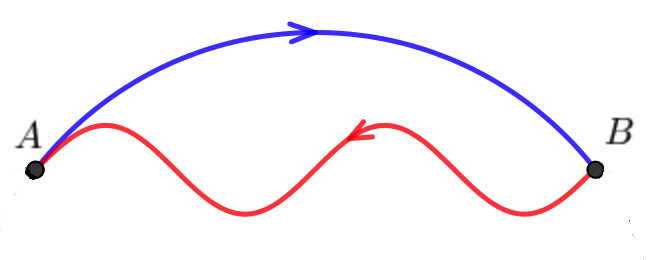
\includegraphics[width=.3\textwidth]{imagenes/imagenes03/T03IM11.png}
		\end{figure}
\end{multicols}

$W_{A\to A}=W_{A\to B}+W_{B \to A}=\mathcal E_p(A)-\mathcal E_p(B) \;+ \; \mathcal E_p(B)-\mathcal E_p(A)=0$

$$ \text{Campo conservativo:}\qquad \oint \vec F \cdot \dd \vec r =0$$

\textcolor{gris}{$\oint$ representa a la integral curvilínea cerrada.}

\rule{150pt}{0.4pt} 

\begin{equation}
\int_A^B \vec F \cdot \dd \vec r = \mathcal E_p(A)- \mathcal E_p(B)=-\int_A^B\dd \mathcal E_p	
\end{equation}

\begin{multicols}{2}
$\dd r = \dd l$, en la dirección de movimiento

$\vec F\cdot \dd \vec r=F\; \dd l\; \cos \theta =-\dd \mathcal E_p $
\begin{figure}[H]
		\centering
		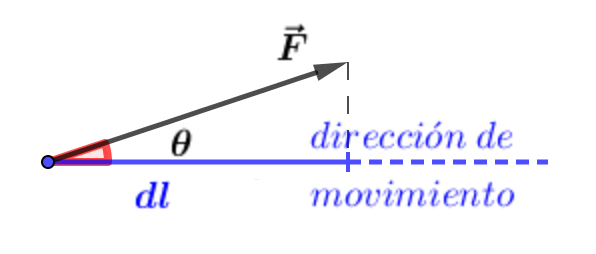
\includegraphics[width=.4\textwidth]{imagenes/imagenes03/T03IM12.png}
		\end{figure}
\end{multicols}

$F \cos \theta=- \dfrac{\dd \mathcal E_p}{\dd l} \; \to \;\; \vec u_r\;F \cos \theta=-\vec u_r\; \dfrac{\dd \mathcal E_p}{\dd l}$

En matemáticas sabemos que un vector $\vec F$ tal que sus componentes, según una dirección determinada del espacio se obtengan a partir de la derivada direccional de una función escalar $\mathcal E_p$, tal vector es el \textbf{\emph{gradiente}} de la función escalar $\mathcal E_p$. (El signo negativo es por convenio).
$$\vec F=-grad\;( \mathcal E_p)$$


$\displaystyle F=\vec i\; F_x +\vec j\; F_y +\vec k\; F_z; \qquad F_x=- \pdv{\mathcal E_p}{x};\; F_y=- \pdv{\mathcal E_p}{y};\; F_z=- \pdv{\mathcal E_p}{z}$


$\displaystyle \vec F=-\left[\;\vec i\;\;\pdv{\mathcal E_p}{x} + \vec j\;\;\pdv{\mathcal E_p}{y} + \vec k\;\;\pdv{\mathcal E_p}{z}\; \right] =$

\begin{equation}
\displaystyle \vec F=- \left( \;\vec i\;\;\pdv{x} + \vec j\;\;\pdv{y} + \vec k\;\;\pdv{z}\; \right)\; \mathcal E_p
\end{equation}

Si llamamos `gradiente' al operador \emph{nabla}: $\displaystyle \grad= \vec i\;\;\pdv{x} + \vec j\;\;\pdv{y} + \vec k\;\;\pdv{z}$

\begin{equation}
\label{Ep-gradiente}
\subrayado{\vec F=-\overrightarrow{ \grad } \mathcal E_p	}
\end{equation}

\emph{\colorbox{LightYellow}{La energía potencial es característica de los campos conservativos.}} 

\emph{En campos no conservativos no tiene sentido hablar de energía potencial.}

$\displaystyle \pdv{F_x}{y}=-\pdv{\mathcal E_p}{y}{x} \quad = \quad -\pdv{\mathcal E_p}{x}{y}=\pdv{F_y}{x} \quad \to \quad \pdv{F_x}{y}-\pdv{F_y}{x}=0$ 

Esto se cumple, por analogía, para las tres componentes:

$\displaystyle \pdv{F_z}{y}-\pdv{F_y}{z}=0 \; \textcolor{gris}{\to\;  \vec i}\;;\quad \pdv{F_z}{x}-\pdv{F_x}{z}=0 \;\textcolor{gris}{\to\;  \vec j}\;;\quad \pdv{F_y}{x}-\pdv{F_x}{y}=0 \;\textcolor{gris}{\to\;  \vec k}$

Y estas son las 3 condiciones que permiten definir matemáticamente a un campo conservativo: \emph{Un campo $\vec F$ es conservativo sus componentes satisfacen simultáneamente las tres ecuaciones anteriores.}

\normalsize{Si} lo escribimos vectorialmente:

$\displaystyle \left( \pdv{F_z}{y}-\pdv{F_y}{z} \right) \;  \vec i+
\left( \pdv{F_z}{x}-\pdv{F_x}{z} \right) \;  \vec j+
\left( \pdv{F_y}{x}-\pdv{F_x}{y} \right) \;  \vec k\;$,

que podemos escribir como:

$\displaystyle \left| \begin{matrix} \vec i&\vec j&\vec k \\ \pdv{x}&\pdv{y}&\pdv{z} \\ F_x&F_y&F_z  \end{matrix} \right|=0 \to \overrightarrow{\grad } \times \vec F = 0$, si hacemos uso del operador nabla.

Cuando el operador nabla actúa como producto vectorial sobre un vector se le llama \textbf{\emph{rotacional}}.


$$\vec F \text{ es conservativo } \leftrightarrow \overrightarrow{\grad } \times \vec F = 0$$ 

\emph{Un campo de fuerzas es conservativo si su rotacional es cero en todos los puntos.}

\textcolor{gris}{Por ejemplo, el campo $\vec F=3x\vec i+5\vec j+7\vec k \to \overrightarrow{\grad } \times \vec F = \left| \begin{matrix} \vec i&\vec j&\vec k \\ \pdv{x}&\pdv{y}&\pdv{z} \\ 3x&5&7  \end{matrix} \right|=0$ y el campo es conservativo}.

\textbf{Teorema de Stookes}: Un campo es conservativo si el trabajo para desplazar la masa activa de un punto $A$ a otro $B$ es independiente del camino elegido.

\begin{equation}
\label{Th-Stookes}
	\vec F \text{\;conservativo} \quad \leftrightarrow \quad  \overrightarrow{\grad } \times \vec F = 0 \quad \leftrightarrow \quad \oint \vec F \cdot \dd \vec r =0
\end{equation}

-- La integral de curvilínea cerrada de $\vec F$ escalarmente por $\dd \vec r$ es cero.

-- El rotacional del campo de fuerzas $\vec F$ es cero en todos los puntos del campo.

Al ser $\vec F=- \overrightarrow{\grad} \mathcal E_p = - \overrightarrow{\grad} \mathcal (E_p+ Cte)$, pues $(Cte)'=0$, tenemos que \emph{la energía potencial es un valor funcional definida salvo una constante arbitraria (origen de energía potencial).} Esa constante no influye en los cálculos pues, al calcular la fuerza la constante desparecen al derivar y al calcular el trabajo, diferencia de energías potenciales, la constante desaparece al restar. Es usual, para campos eléctricos y gravitatorios, escoger esa constante de modo que se anule para puntos alejados de la partícula que crea en campo ($\mathcal E_p \to 0$ cuando $r\to \infty$).
 
 
 \emph{Tanto la energía cinética como la potencial dependen del sistema de referencia elegido.}

\rule{150pt}{0.4pt} 

En el ejemplo anterior, $\vec F = 3x\vec i + 5 \vec j+7\vec k=\displaystyle - \overrightarrow{\grad} \mathcal E_p$, es fácil obtener que el funcional energía potencial es $\mathcal E_p=3\frac{x^2}2+5y+7j+\mathcal K$, con $\mathcal K$ la constante arbitraria.

$\mathcal E_p(2,-3,1)=6-15+7=-2$, si deseamos que el origen de potencial este en el punto $(2,-3,1)$, definiremos la energía potencial como: $E_p=3\frac{x^2}2+5y+7j-2$.

\rule{150pt}{0.4pt} 



\subsection{Energía potencial gravitacional}

La energía potencia gravitacional es la asociada al peso de un cuerpo y a su altura sobre el suelo. Consideraremos que la altura sobre la superficie de la tierra es tal que puede considerarse la fuerza peso constante [$g=g(r)$].

\vspace{30mm} %****************************************
\begin{multicols}{2}
Calculemos el trabajo que efectúa la fuerza peso (única presente) para bajar un cuerpo de masa $m$ desde la posición $y_1$ hasta la $y_2$ a $v=cte$ (proceso \textit{a)} en la figura adjunta). La fuerza es paralela al desplazamiento $\dd W=\vec F\cdot \dd \vec r$. Como la fuerza y es desplazamiento son paralelos y del mismo sentido ($+\vec j$):

\begin{figure}[H]
		\centering
		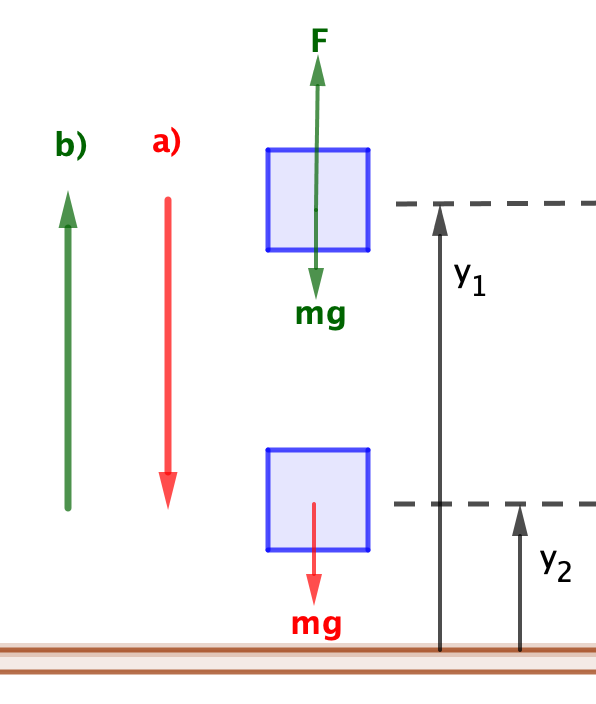
\includegraphics[width=.25\textwidth]{imagenes/imagenes03/T03IM54.png}
		\end{figure}
\end{multicols}

 $W=F\cdot \Delta y=mg(y_1-y_2)>0$ (movimiento en eje $Y$).
 
 El trabajo es positivo, lo realizan las fuerzas del campo y el movimiento es espontáneo.
 
 Llamamos \emph{energía potencial (gravitacional)} de una partícula, de masa $m$ a una altura $y$ sobre el origen de energías potenciales que se tome, como:

\begin{equation}
	\label{EP-gravitacional}
	\subrayado{\mathcal E_p=mgy}
\end{equation}

Lueqo: $W_{1\to 2}=mgy_1-mgy_2=\mathcal E_{p_1}-\mathcal E_{p_2}=-(\mathcal E_{p_2}-\mathcal E_{p_1})=-\Delta \mathcal E_p$

En el caso \textit{b)} de la figura, subrir el cuerpo de la posición $2$ a la $1$, tenemos:
$\ W_{2\to 1}=-\Delta \mathcal E_p (2 \to 1)=-(\mathcal E_{p_1}-\mathcal E_{p_2})=-(mgy_1-mgy_2)=mh(y_2-y_1)<0$

Ahora, el $W<0$, debe existir una $\vec F$ externa que realice el trabajo contra las fuerzas del campo (gravitatorio).

\subsection{Energía potencial elástica} \label{Hooke}
Supongamos un muelle en el que llamamos $0$ a su posición de equilibrio y lo desplazamos una pequeña distancia $x \vec i$ de ésta (pequeña para que se verifique la Ley de Hooke). 
\begin{multicols}{2}
Actúa sobre él una fuerza que trata de devolverlo a su posición inicial: $\vec F=-K x \vec i$, con $k$ la constante de elasticidad del muelle y el signo menos denota que tiende a devolver al muelle a su posición inicial.
\begin{figure}[H]
		\centering
		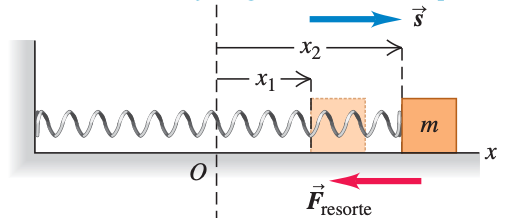
\includegraphics[width=.5\textwidth]{imagenes/imagenes03/T03IM55.png}
		\end{figure}
\end{multicols}
Sabemos que $F=-\dv{\mathcal E_p}{x}=-k x \to \dd \mathcal E_p= kx \dd x$

Tomamos el origen de energía potencial en la posición $0$ de equilibrio del muelle, integrando:

$\displaystyle \int_0^{\mathcal E_p} \dd \mathcal E_p=\mathcal E_p=\int_0^x k x \dd x= \dfrac 1 2 k x^2$

Para un muelle de constante $K$ alejado una distancia $x$ de su posición de equilibrio, \emph{llamamos energía potencial elástica} a la expresión:

\begin{equation}
	\label{EP-gravitacional}
	\subrayado{\mathcal E_p=\dfrac 1 2 k x^2}
\end{equation}

Analicemos los casos posibles:

El muelle vuelve desde su posición $x_2$ más alejada a la posición $x_1$ más próxima a la posición de equilibrio:

$W_{2 \to 1}=-\Delta \mathcal E=-(\mathcal E_{p_1}-\mathcal E_{p_2}=\mathcal E_{p_2}-\mathcal E_{p_1}=\dfrac 1 2 k x_2^2- \dfrac 1 2 k x_1^2=\dfrac 12 k (x_2^2-x_1^2)>0 \quad (x_2>x_1>0)$, por lo que el sistema evoluciona libremente desde $x_2$ hasta $x_1$.

El trabajo necesario para estirar al muelle desde $x_1$ hasta $x_2$ será:

$W_{1 \to 2}=-\Delta \mathcal E_p (1 \to 2)=-(\mathcal E_{p_2}-\mathcal E_{p_1}=\mathcal E_{p_1}-\mathcal E_{p_2}=\dfrac 1 2 k (x_1^2-x_2^2)<0$. Una fuerza externa debe actuar para desarrollar este trabajo contra las fuerzas del campo elástico.

\vspace{10mm} %********************************* 
\begin{figure}[H]
	\centering
	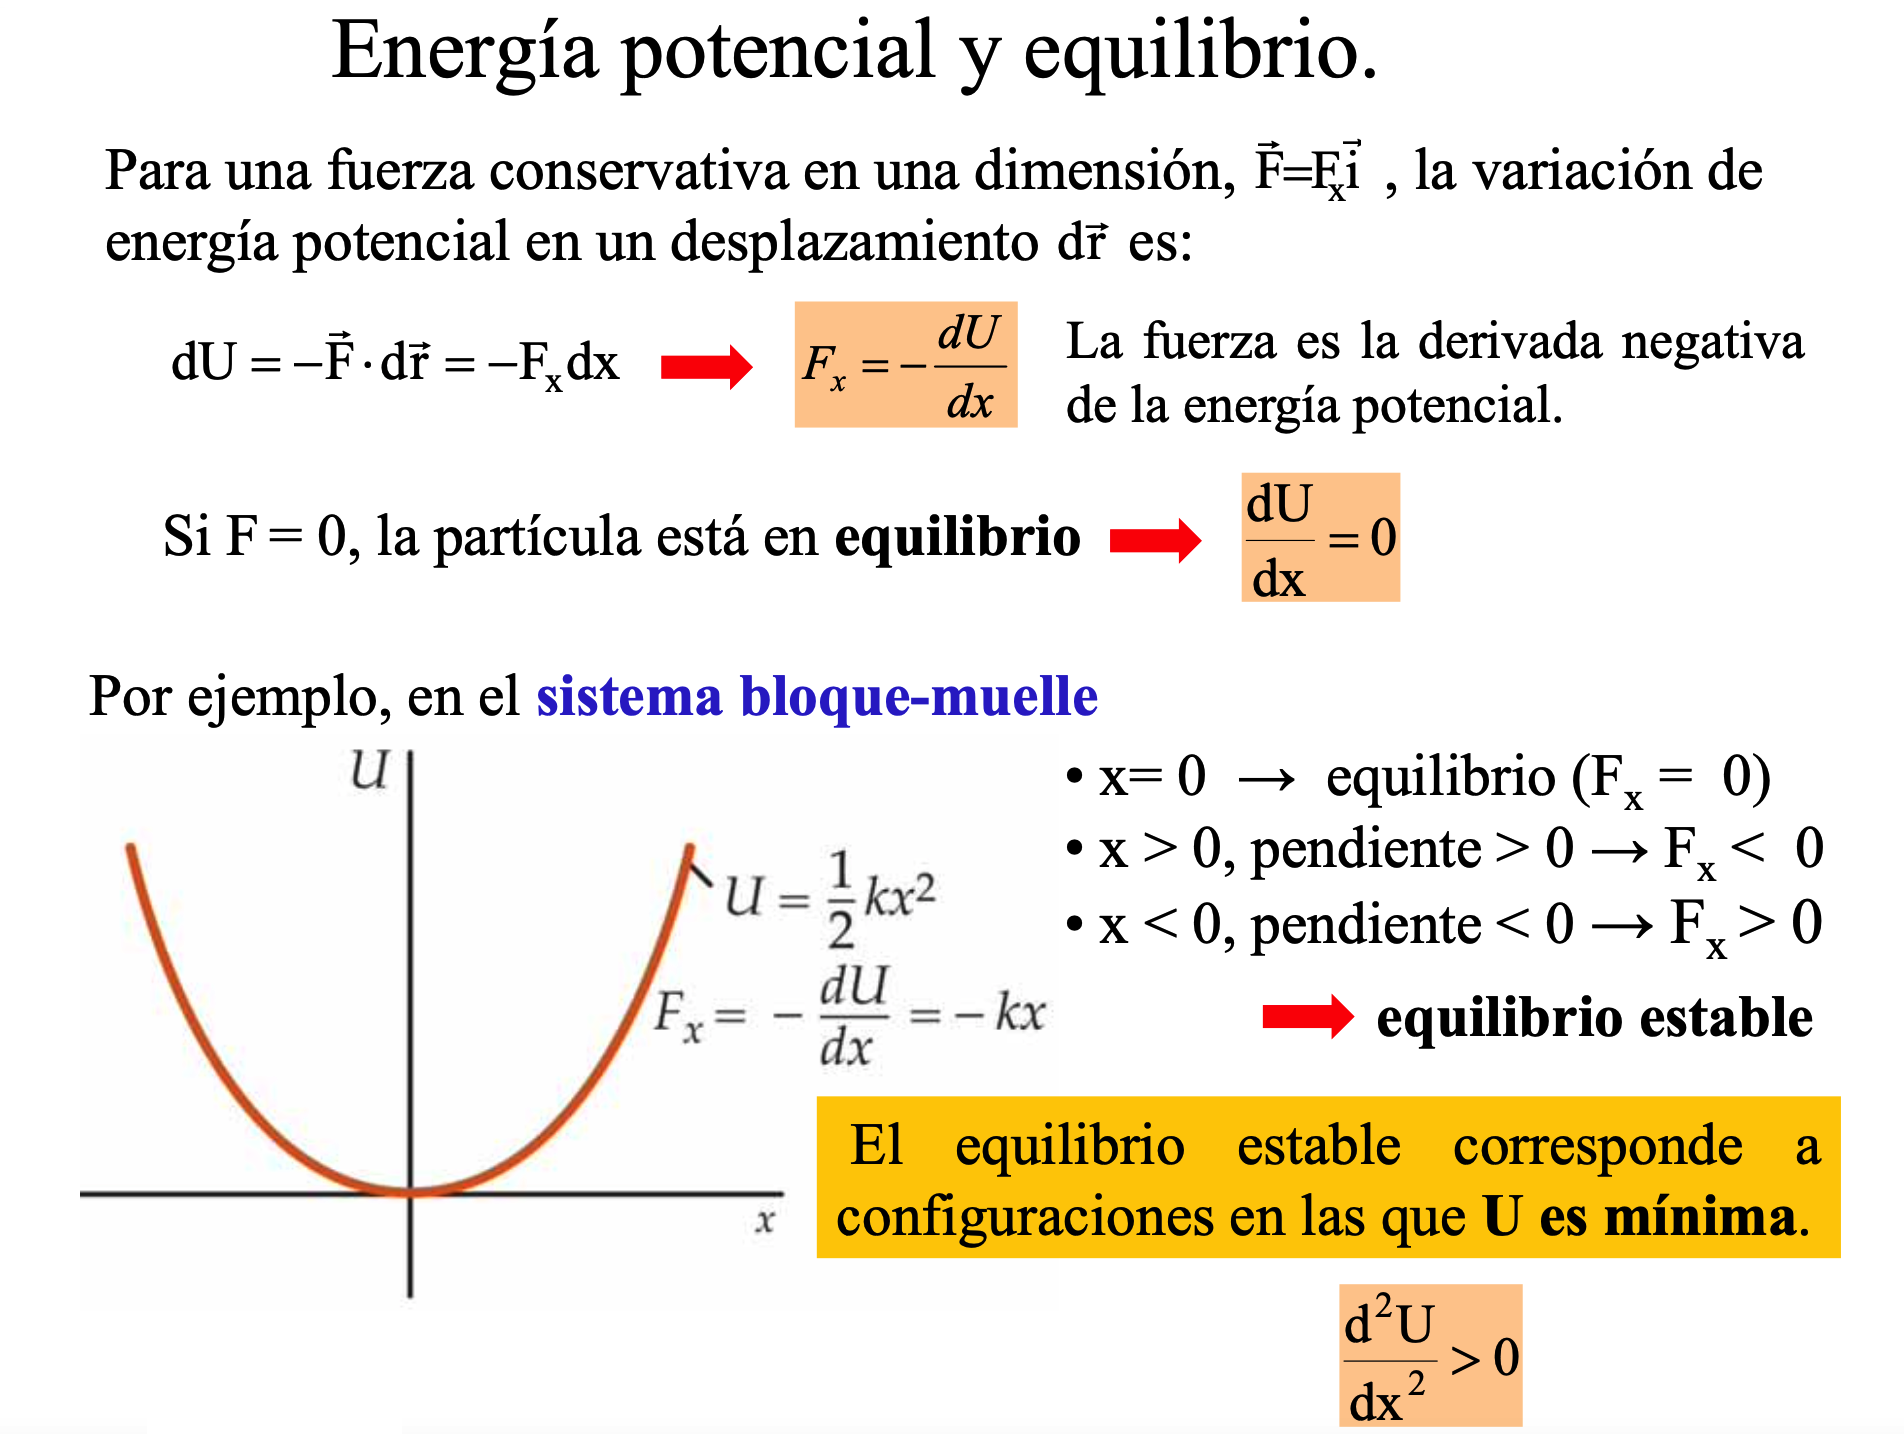
\includegraphics[width=.95\textwidth]{imagenes/imagenes03/T03IM50.png}
	\end{figure}
	
\begin{figure}[H]
	\centering
	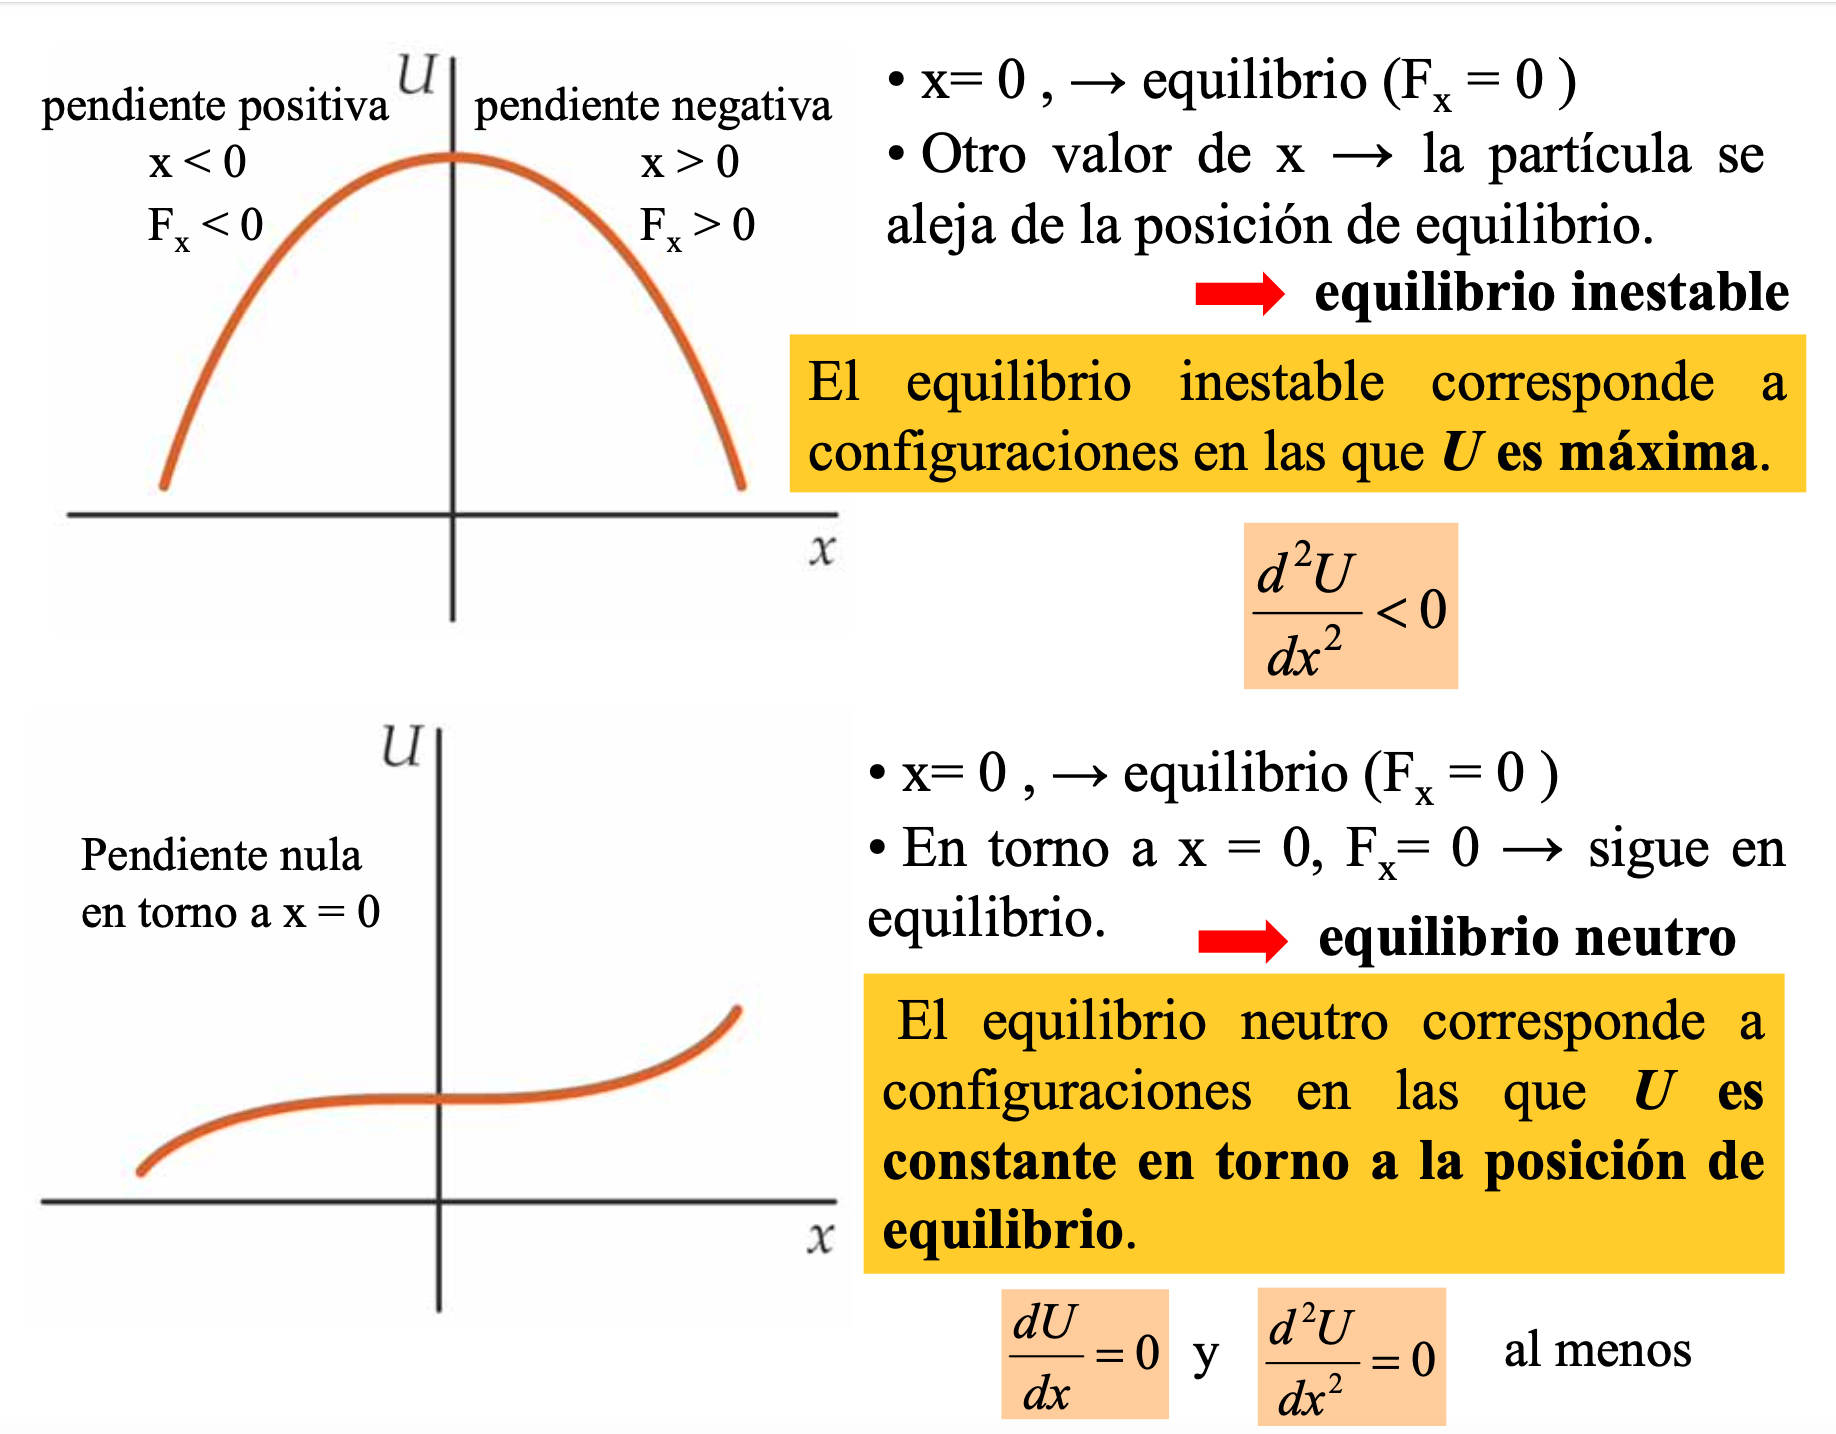
\includegraphics[width=.95\textwidth]{imagenes/imagenes03/T03IM51.png}
	\end{figure}


\subsection{Significado físico-matemático del gradiente}
\label{potenciales-decrecientes}
\begin{multicols}{2}
Supongamos una región del campo en que $\mathcal E_p(x,y,z)=cte$, matemáticamente esto es una \emph{superficie}.
\begin{figure}[H]
		\centering
		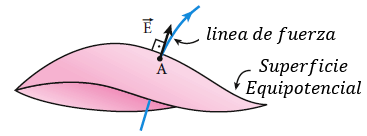
\includegraphics[width=.5\textwidth]{imagenes/imagenes03/T03IM14.png}
		\end{figure}
\end{multicols}

$\mathcal E_p(x,y,z)=cte \to - \overrightarrow{\grad} \mathcal E_p = 0 = \vec F \cdot \dd \vec r \to \left( \; \vec F \;\parallel \; \overrightarrow{\grad}  \mathcal E_p \; \right) \; \; \bot \; \; \dd \vec r$

El vector $\vec F$ o el vector gradiente es \emph{perpendicular} a la superficie equipotencial.

Sea $\vec u_R$ un vector unitario en la dirección en que actúa la fuerza sobre la magnitud activa. Como
$\vec F = \vec u_R \; F=- \vec u_R \; \dv{\mathcal E_p}{R}\;$
para que $F>0$, $\dv{\mathcal E_p}{R} <0$. La fuerza está orientada em el sentido de potenciales decrecientes: $\mathcal E_{p_2} < \mathcal E_{p_1} \to \dd \mathcal E_p < 0$

El vector fuerza (y el vector gradiente de energía potencial) es perpendicular a las superficies equipotenciales en cada punto y está orientado hacia los potenciales decrecientes.
\vspace{-5mm}\begin{figure}[H]
		\centering
		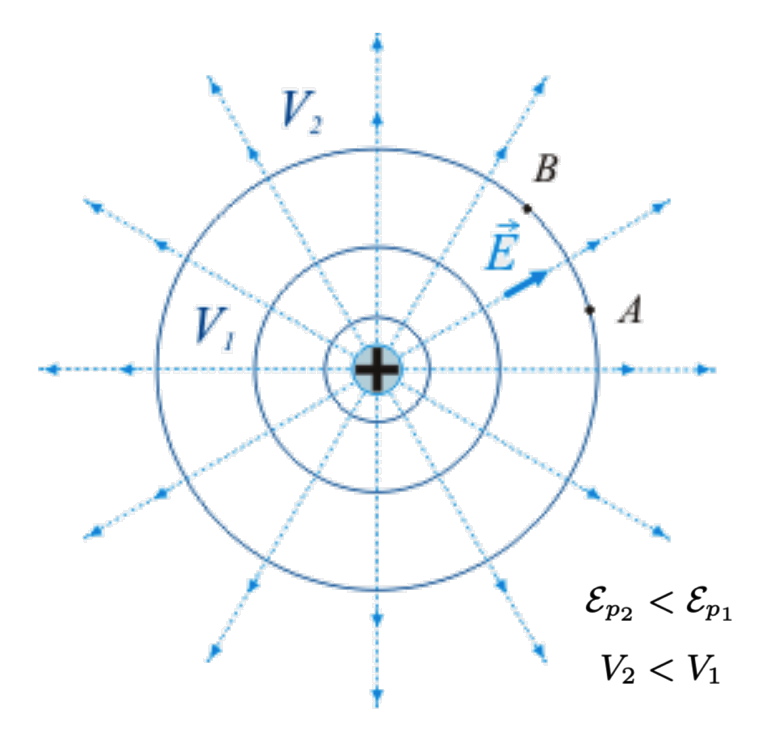
\includegraphics[width=.4\textwidth]{imagenes/imagenes03/T03IM15.png}
		\end{figure}


\section{Problemas}

\begin{prob}
Una partícula de $100 \ \mathrm{g}$ se lanza con una velocidad inicial de $100 \ \mathrm{ms}^{-1}$ en una región del espacio que le ofrece una resistencia  $F=0.25\ v^2\ \mathrm{N}$, si $v$, velocidad instantánea de la partícula, se expresa en $\mathrm{ms}^{-1}$. Considerando el movimiento unidimensional, averiguar la velocidad que lleva la partícula cuando ha recorrido $1\ \mathrm{m}$, así como el tiempo empleado en recorrerlo.
\end{prob}

$F$ ofrece resistencia al movimiento, se opone a él: 

$F=-0.25 v^2=-Av^2$; $\quad A=0.25\ \dfrac{\mathrm{N}}{\mathrm{m}^2\mathrm{s}^2}=0.25 \dfrac{\mathrm{kg}}{\mathrm{m}}$

$F=ma\ \to \ a=\dfrac F m = \dfrac {-A} m v^2 =\displaystyle \dv{v}{t}$

$\displaystyle \int_{v_0}^v \dfrac{\dd v}{v^2}=-\dfrac A m  \int_0^t \dd t \to \ \dfrac 1 {v_0}-\dfrac 1 v =-\dfrac A m \ t $

$\boldsymbol{v(t)=\left(\dfrac 1 {v_0}+\dfrac A m\ t \right)^{-1}}$

$v(t)=\displaystyle \dv{r}{t}\to \ \int_0^r \dd r = \int_0^t \left(\dfrac 1 {v_0}+\dfrac A m\ t \right)^{-1}\dd t$

$r=\displaystyle \int_0^t \dfrac{mv_0}{m+At}\dd t= \dfrac{mv_0}{\boldsymbol {A} }\int_0^t \dfrac{\boldsymbol{ A}}{m+At} \dd t= \dfrac{mv_0}{A} \eval {\ln(m+At)}_0^t \to $

$\boldsymbol{r= \dfrac {mv_0}{A} \ln \dfrac {m+At}{m}}$


Despejando: $\displaystyle \dfrac {rA} {mv_0} =\ln \dfrac {m+At}{m}; \quad \dfrac {m+At}{m} = e^{ \dfrac {rA} {mv_0} } $

Por último: $\quad \boxed{ \displaystyle t=\dfrac {m}{A}\ \left[ e^{\dfrac{rA}{mv_0}} - 1 \right] }$

De ahí, $\quad \boxed{ v=}\left(
\dfrac 1 {v_0}+\dfrac A m \dfrac {m}{A} 
 \left[ e^{ \dfrac{rA}{mv_0} } - 1  \right] 
\right)$
$=\boxed{ \left(  \dfrac 1 {v_0} + e^{\dfrac{rA}{mv_0}} - 1 \right)^{-1} }$

Solo queda sustituir valores para obtener $\quad t=0.011\ \mathrm{s};\quad v=97.53\ \mathrm{ms}^{-1}$

\textcolor{gris}{$0.25 \mathrm{kgm}{-1}; \quad v_0=100\ \mathrm{ms}^{-1};\quad m=0.1\ \mathrm{kg};\quad r=1\ \mathrm{m}$}

%\rightline{\textsf{\textcolor{DarkBlue}{--- Inacabado ---}}}


\begin{prob}
Una cadena está sobre una mesa sin fricción con la quinta parte de su longitud colgando de un borde. La cadena tiene una masa $M$ y una longitud $L$, ?`cuánto trabajo se requiere para subir la cadena a la mesa?	
\end{prob}

\begin{multicols}{2}
La única fuerza que actúa es la de la gravedad que es una fuerza central y, por ello, conservativa $\to W= \int_A^B \dd \mathcal E_p$.

Suponemos la cadena homogénea: $\lambda=\frac M L$, con $\lambda$ la densidad lineal.
\begin{figure}[H]
	\centering
	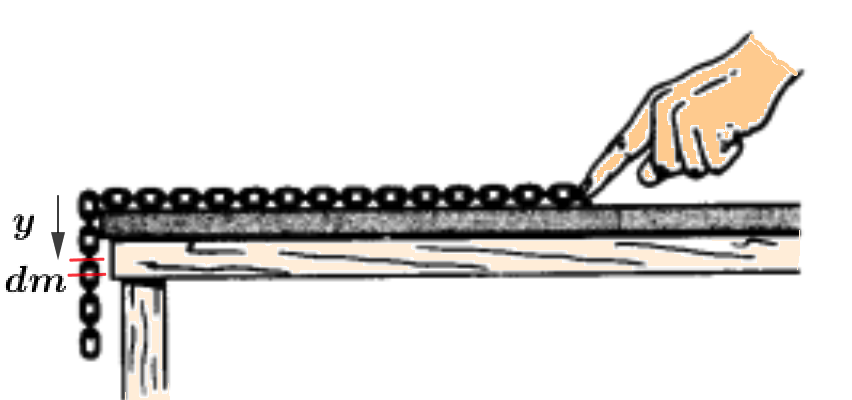
\includegraphics[width=.5\textwidth]{imagenes/imagenes03/T03IM33.png}
	\end{figure}
\end{multicols}
Una porción infinitesimal de cadena colgante es $\dd m$ y está a una altura $y$ del borde de la mesa, con $y\in [0,l]$ (en nuestro caso $l=L/5$).

Tenemos que $\dd m=\lambda \; \dd y =\frac M L \; \dd y$. La energía potencial de este elemento de cadena es: $\dd \mathcal E_p=\dd m \; g \; y=\frac M L \ g \ y \ \dd y$.

El trabajo para subir el trozo de cadena a la mesa lo obtendremos sumando (integrando) para todos los elementos de cadena desde la posición $l$ hasta la posición $0$:

$W=\displaystyle \int_l^0 \dd \mathcal E_p=\int_l^0 \frac M L \ g \ y \ \dd y=\frac M L \ g \ \eval{y\ \dd y}_l^0=- \frac M L \ g\ \frac {l^2}{2}$

En nuestro caso, $l=L/5 \to  W=-\displaystyle \dfrac{M\ g\ L }{50}$

El sentido negativo indica que el trabajo se efectúa contra las fuerzas del campo. Hay que realizar este trabajo externo para que la cadena suba a la mesa.

\textcolor{gris}{Comprobación dimensional: $-\dfrac{M\ g\ L }{50} \to 
[\mathrm{M}][\mathrm{LT}^-{2}][\mathrm{L}]=[\mathrm{ML}^2\mathrm{T}^{-2}]\to \mathrm{W}$}


\textcolor{gris}{\textsf{Hubiésemos podido resolver el problema imaginando el trozo $L/5$ de cadena, de peso $M/5$ como una partícula de masa $M/5$ a una distancia $-\frac 1 2 \ \frac L 5=-\frac {L}{10}$ por debajo de la superficie de la mesa (toda la masa del extremo colgante de la cadena concentrada en su centro de gravedad, a la mitad de su longitud). En estas condiciones, $\mathcal E_p=m \ g \ h=\frac M 5 \ g \ \left( -\frac L {10} \right) = -\dfrac{M\ g\ L }{50}$.}}

\textbf{análisis de caso límites.} $W=-\dfrac M L g \dfrac {l^2}2$
\begin{itemize}
\item $l=L \to W=-\dfrac M L g \dfrac {L^2}2=-Mg\dfrac L 2$. Es como si toda la cadena estuviese colgando a distancia $L/2$ del borde de la mesa (lo que concuerda si la usamos la aproximación de considerarla como una partícula centrada en su c.d.g\footnote{centro de gravedad.})
\item $l=0 \to W=0$, toda la cadena está sobre la mesa y no hay que realizar ningún trabajo para subirla.
\end{itemize}


\begin{prob}
Una ametralladora dispara balas de $50\ \mathrm{g}$ con una velocidad de $10^3\ \mathrm{ms}^{-1}$. El soldado que sostiene la ametralladara en sus manos puede ejercer una fuerza meia de $180\ \mathrm{N}$ contra el arma. Determínese el número máximo de balas que puede disparar en $1 \mathrm{min}$.	
\end{prob}

$F=\displaystyle \dv{t} (mv)=\dv{m}{t} v + m \cancelto{0}{\dv{v}{t}}=\dv{m}{t} v$, la velocidad no varía al salir del  arma.

$\overline{F} \displaystyle =\dfrac 1 T \int_0^T F \dd t=\dfrac 1 T \int_0^T \dv{m}{t} \ v\  \dd t=\dfrac 1 T \int_0^T v\  \dd m= \dfrac 1 T\  v \int_0^T \dd t = \dfrac v m T$

$T=60 \ \mathrm{s}; \quad \overline{F}=180\ \mathrm{N}; \quad M=n\ m \to \ \overline{F}=\dfrac v T \ n \ m$

Luego $\ \ n=\dfrac {\overline{F} \ T}{m \ v}= \dfrac{180 \cdot 60}{10^3 \cdot 5\ 10^{-2}}=216\ $balas en un minuto.


\begin{prob}
Una partícula de masa $m$ se mueve	en línea recta sometida a una fuerza constante de módulo $F$ y a una resistencia $kv^2$, donde $v$ es la velocidad. Si en el instante inicial la partícula tiene velocidad $v_0$, ?`qué distancia habrá recorrido cuando lleve velocidad $v$? ?`Cuál es la velocidad límite de la partícula? 
\end{prob}

$2^a$ de Newton: $\displaystyle \ \ F-kv^2=ma=m \dv{v}{t}=m\dv{v}{s} \dv{s}{t}=mv\dv{v}{s}$

$(F-kv^2)\ \dd s= mv\ \dd v \to \ \ \dd s=\dfrac{mv}{F-kv^2}\dd v$, integrando:

$s=\displaystyle \int_0^s \dd s= -\dfrac m{2k} \int_{v_0}^v \dfrac{-2k\ v\ \dd v}{F-kv^2} =-\dfrac m{2k} \eval{\ln (F-kv_2)}_{v_0}^v  \to$

$\displaystyle s=\dfrac m{2k} \ \ln \dfrac{F-kv_0^2}{F-kv^2}$

La velocidad límite se alcanzará cuando: 

$\ a=cte \to F_{total}=0 \to F-kv^2=0 \Rightarrow v_L=\sqrt{\dfrac{F}{K}}$

\textcolor{gris}{De otro modo: $\ v_L \ $ se alcanzará cuando $\ s\to +\infty \ $ es decir, cuando  $\ \dfrac m{2k} \ \ln \dfrac{F-kv_0^2}{F-kv} \to + \infty$ ; lo que ocurrirá cuando el denominador tienda a cero: $F-kv^2 \to 0$, luego: $v_L=\sqrt{\dfrac{F}{K}}$}.

\begin{prob}
Un vagón cargado de arena tiene un agujero en el fondopor el que ésta sale con una rapidez constante $w=-\dd m / \dd t$. Una fuerza constante actúa sobre el vagón en la dirección de su movimiento. Determínese la ecuación del movimiento y la velocidad instantánea del vagón.	
\end{prob}

$\displaystyle w=-\dv{m}{t} \to \dd m = -w \dd t ;\ \ \int_{m_0}^m \dd m=-w \int_0^t \dd t \Rightarrow \quad m=m_0-wt$

$\displaystyle F=cte=\dv{p}{t}=\dv{mv}{t}=\dv{m}{t}v+m\dv{v}{t}=-wv+m\dv{v}{t}$

Multiplicando por $\dd t$ 

$\displaystyle F\dd t=-wv\dd t + m \dd v \to (F+wv)\dd t=(m_o-wt)\dd v$

Separando variables e integrando: 

$\displaystyle - \dfrac 1 w \int_0^t (-w)\ \dfrac{\dd t}{m_0-wt}=\dfrac 1 w \int_{v_0}^v (w) \ \dfrac{\dd v}{F+mv}$

$\displaystyle -\ln \eval{(m_0-wt)}_0^t=\ln \eval{(F+wv)}_{v_0}^v \to
\dfrac{F+wv}{F+wv_0}=\dfrac{m_0}{m_0-wt}$, 

despejando:
$\displaystyle v=\dfrac{m_0v_0+F}{m_o-wt}=\quad \dv{s}{t}$

luego: $\displaystyle \dd s= \dfrac{m_ov_0+F}{m_0-wt} \ \dd t$, integrando:

$\displaystyle s=\int_0^s \dd s= -\dfrac 1 w \int_0^t (-w) \dfrac{m_0v_0+F}{m_0-wt} \dd t \Rightarrow \quad s=\dfrac 1 w \ln \dfrac {m_0}{m_0-wt}$

\vspace{10mm} %*****************************************
\begin{prob}
	\begin{multicols}{2}
$\quad$

$\quad$

Calcúlese las fuerzas normal y tangencial que actúan sobre un proyectil lanzado horizontalmente desde una altura $h$	.
\begin{figure}[H]
		\centering
		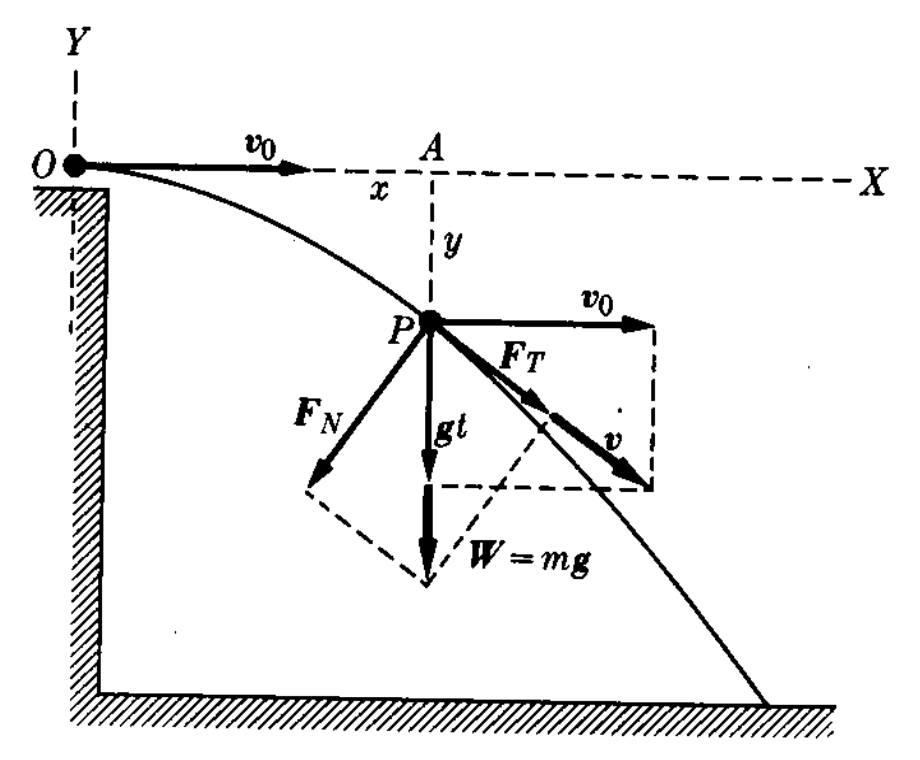
\includegraphics[width=.45\textwidth]{imagenes/imagenes03/T03IM57.png}
		\end{figure}
	\end{multicols}
\end{prob}


$MRUA:\quad \left| \begin{matrix}\ a_x=0 \quad \  \\ \ a_y=-g \     \end{matrix} \right|
\left. \begin{matrix}  v_x=v_0 \quad \ \\ v_y=-gt  \   \end{matrix} \right|
\left. \begin{matrix} x=v_0t  \quad \quad \quad \quad \ \\ y=h-gt-\frac 1 2 g t^2     \end{matrix} \right.$

De las ecuaciones de velocidades: $v=\sqrt{v_x^2+v_y^2}=\sqrt{v_0^2+g^2t^2}$

Fuerza tangencial: $\ F_T=\displaystyle m \dv{v}{t}=\dfrac{mg^2t}{\sqrt{v_0^2+g^2t^2}}$

Para encontrar la fuerza normal usando la ecuación $\ F_N=\displaystyle m\dfrac{v^2}{\rho}$, necesitaríamos conocer el radio de curvatura en $\rho$ en cualquier instante; la partícula describe una parábola. De otro modo, podemos hacer:

$F=\sqrt{F_T^2+F_N^2}=mg \to F_N=\sqrt{mg-F_T^2}=\dfrac{mgv_0}{\sqrt{v_o^2+g^2t^2}}$

\begin{prob}
Un astronauta que construye una estación espacial empuja un bloque de masa $m_1$ con una fuerza constante $F$. Este bloque está en contacto directo con un segundo bloque de masa $m_2$. Determina la aceleración en los bloques así como el módulo de la fuerza que ejerce cada bloque sobre el otro.	
\end{prob}

\vspace{30mm} %**********************************************
\begin{multicols}{2}
\begin{figure}[H]
	\centering
	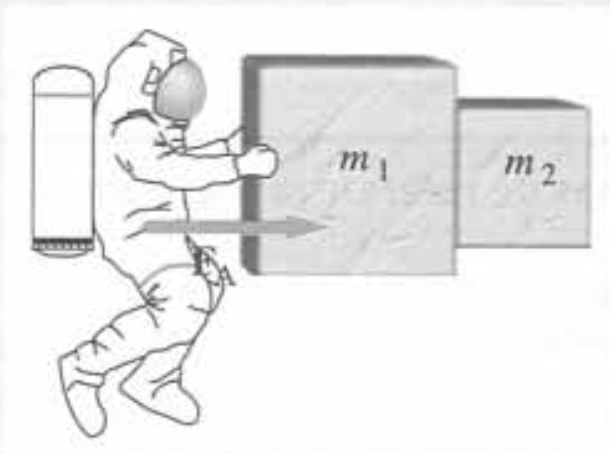
\includegraphics[width=.5\textwidth]{imagenes/imagenes03/T03IM59.png}
	\end{figure}
$\quad$
\begin{figure}[H]
	\centering
	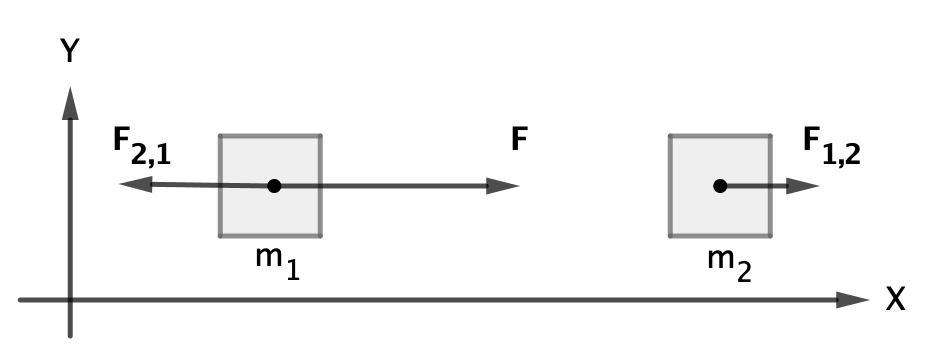
\includegraphics[width=.5\textwidth]{imagenes/imagenes03/T03IM60.png}
	\end{figure}
\end{multicols}	

A la derecha del astronauta hemos representado los diagramas de fuerzas de cuerpo libre de los dos bloques.

Llamamos $R$, de fuerza de reacción, a $R=|\vec F_{1,2}|=|\vec F_{2,1}|$

$m_1: \quad F-R=m_1 a; \qquad \qquad m_2: \quad R=m_2 a$

De donde: $\quad a=\dfrac{F}{m_1+m_2};\qquad R=\dfrac{m_2}{m_1+m_2}F$



\begin{prob}
Analizar el efecto de la rotación de la tierra sobre un cuerpo.
\end{prob}

Llamamos $W_G$ a la fuerza gravitacional ejercida a la atracción de la tierra. Si la tierra no rotara, la aceleración que sentiría un cuerpo cerca de la superficie terrestre sería $a=W_G/m$, pero debido a la rotación, parte de de esta fuerza se ha de dedicar la fuerza normal necesaria para que el punto $A$ describa una trayectoria circular de radio $\overline{CA}=r\cos \lambda$ con velocidad angular $\omega$, $\ F_N=m\omega^2 r$. 
\begin{multicols}{2}
La diferencia $W_G-F_N$ nos da la fuerza total $W$ que actúa hacia abajo sobre la partícula de modo que la \emph{aceleración efectiva} de la gravedad que siente ésta es $g=W/m$.

Si la partícula $A$ estuviese suspendida de un hilo como una plomada, la cuerda tendría la dirección de $W$. Este es el motivo por el que las plomadas no apuntan al centro de la tierra, si ésta parase de rotar veríamos a todos los edificios inclinados. Solo en el ecuador y en los polos $W$ y $W_G$ tienen la misma dirección y solamente allí la dirección de la plomada es radial.
\begin{figure}[H]
	\centering
	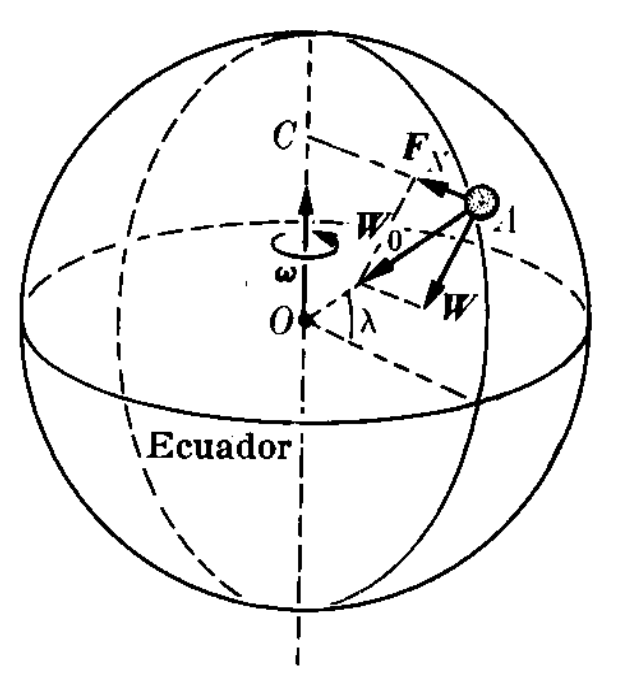
\includegraphics[width=.4\textwidth]{imagenes/imagenes03/T03IM58.png}
	\end{figure}
\end{multicols}


\vspace{30mm} %**************************************

\begin{prob}.
\begin{multicols}{2}
Una persona de $80 \ \mathrm{kg}$ está de pie sobre una balanza, sujeta al suelo de un ascensor. La balanza está calibrada en $\mathrm{N}$. ?`Qué peso indicará la balanza cuando a) el ascensor se mueva con aceleración $a$ hacia arriba; b) el ascensor se mueva con aceleración $a'$ hacia abajo; c) el ascensor se mueva hacia arriba a $20\ \mathrm{ms}^{-1}$, mientras su velocidad decrece a razón de $8\ \mathrm{ms}^{-2}$; d) si se rompe el cable del ascensor.

Lo que mide la bascula es la reacción normal a la fuerza que soporta. En el dibujo aparece el peso como $\omega=mg$.
	\begin{figure}[H]
	\centering
	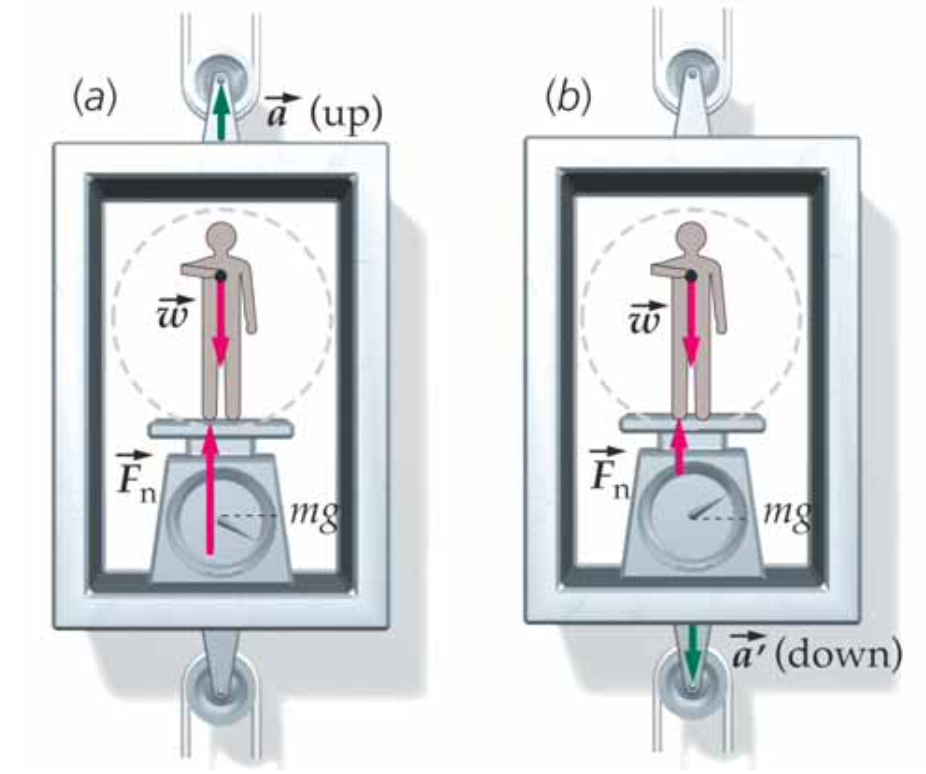
\includegraphics[width=.45\textwidth]{imagenes/imagenes03/T03IM21.png}
	\end{figure}
\end{multicols}
\end{prob}
--- a) $\quad \uparrow a \to \Sigma F= N-mg = ma \to N=mg+ma=m(g+a)$

--- b) $\quad \downarrow a \to \Sigma F= N-mg = -ma \to N=mg-ma=m(g-a)$

--- c) $\quad \uparrow a:\quad \Sigma F=m(g-a)=80(9.8-8)=144\; \mathrm{N}$

--- d) $\quad \downarrow a=g \to \Sigma F= N-mg = -mg \to N=0$

El peso que mide la báscula es la reacción de soporte que ofrece al hombre. En caída libre, tanto hombre como báscula notan la sensación de ingravidez. 


\footnotesize{\textsf{Peso aparente e ingravidez aparente.}}
 
\footnotesize{\textsf{Generalicemos los resultados . Cuando un pasajero de masa $m$  viaja en un elevador con aceleración $a_y$  una báscula da como peso aparente del pasajero $N=m(g+a_y)$.}}

\footnotesize{\textsf{Cuando el elevador está acelerando hacia arriba, $a_y$   es positiva y $N$ es mayor que el peso del pasajero $ \textit{w} = mg$. Si el elevador acelera hacia abajo, $a_y$   es negativa y $N$ es menor que el peso. Si el pasajero no sabe que el elevador está acelerando, sentirá que su peso cambia y, de hecho, la báscula asá lo indica.}} 

\footnotesize{\textsf{El caso extremo sucede cuando el elevador tiene una aceleración hacia abajo  $a_y=-g$, es decir, cuando está en caída libre. En este caso, $N=0$  y el pasajero siente que no tiene peso. Asimismo, un astronauta en órbita alrededor de la Tierra experimenta ingravidez aparente. En ambos casos, la persona aún tiene peso, porque actúa sobre ella una fuerza gravitacional; sin embargo, el efecto de esta condición de caída libre es el mismo que si el cuerpo estuviera en el espacio exterior sin experimentar gravedad. En ambos casos, la persona y su vehículo (elevador o nave) están cayendo juntos con la misma aceleración $g$, así que nada empuja a la persona contra el piso o las paredes del vehículo}}\normalsize{.}

\begin{prob}
Cuando una avión acelera en la pista de una aeropuerto para despegar, un viajero decide determinar la aceleración mediante un yo-yo comprobado que éste se separa de la vertcial un ángulo de $22^o$. ¿Cuál es la aceleración del avión?. Si la masa del yo-yo es de $40\ \mathrm{g}$, ?`cuál es la tensión en el hilo?	
\end{prob}

\vspace{30mm} %**************************************

\begin{multicols}{2}
La fuerza neta sobre el yo-yo es en la dirección de la aceleración y la suministra la componente horizontal de la tensión. La componente vertical equilibra el peso.

$\Sigma F_x: \ \ T \cos \theta-mg=0$

$\Sigma F_y: \ \ T \sin \theta = m a$

Despejando:  
$a=g \tan \theta; \quad T=\dfrac{mg}{\cos \theta}$

\begin{figure}[H]
	\centering
	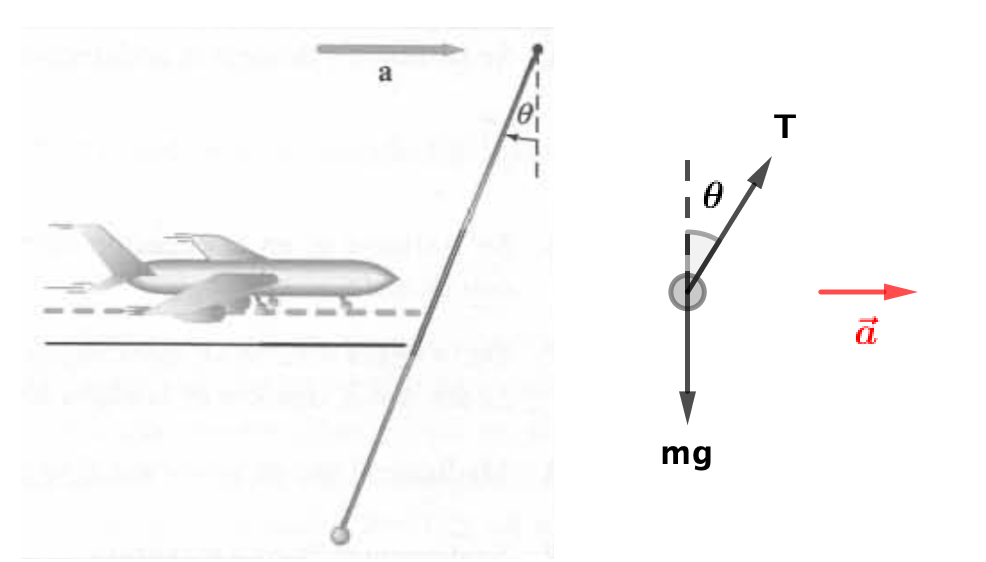
\includegraphics[width=.5\textwidth]{imagenes/imagenes03/T03IM64.png}
	\end{figure}
\end{multicols}	
Para los datos del problema:  
$\ \ a=3.96\ \mathrm{ms}^{-2}; \quad T=0.423\ \mathrm{N}$
	
\begin{prob}
\begin{multicols}{2}
Un elevador y su carga tienen masa total de $800 \mathrm{kg}$  y originalmente está bajando a $10.0 \ \mathrm{ms}^{-1}$; se le detiene con aceleración constante en una distancia de $25.0 \mathrm{m}$. Calcule la tensión T en el cable de soporte mientras el elevador se está deteniendo.	
\begin{figure}[H]
	\centering
	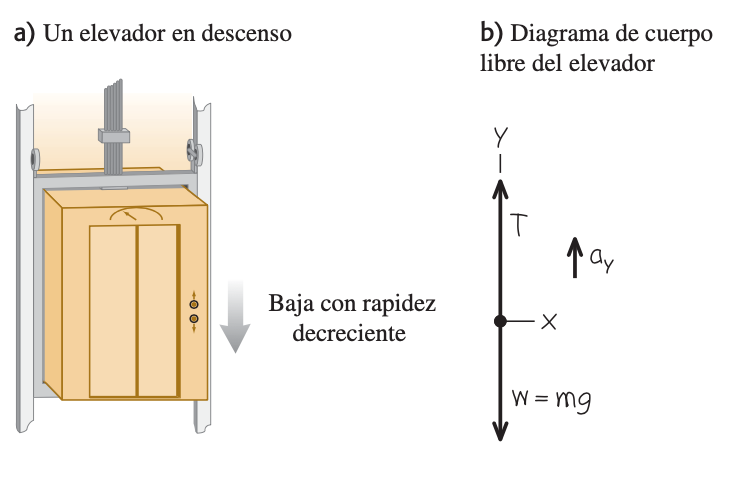
\includegraphics[width=.4\textwidth]{imagenes/imagenes03/T03IM39.png}
	\end{figure}
\end{multicols}
\end{prob}
$\Sigma F_y=t-mg=ma_y \to T=m(g+a_y)$
$ \quad \begin{cases} v=v_0+at \\ x=x_0+v_0 t + \frac 1 2 a t^2  \end{cases} \to a=2\ \mathrm{m s}^{-2}$ $\qquad T=9440\ \mathrm{N}$


\vspace{10mm} %************************************
\begin{prob}
En la figura, un deslizador de masa $m_1$ se mueve sobre un riel de aire horizontal, sin fricción, en el laboratorio de física. El deslizador está conectado a una pesa de masa $m_2$ mediante un cordón ligero, flexible e inelástico que pasa por una pequeña polea sin fricción. Calcule la aceleración de cada cuerpo y la tensión en el cordón.	
\begin{figure}[H]
	\centering
	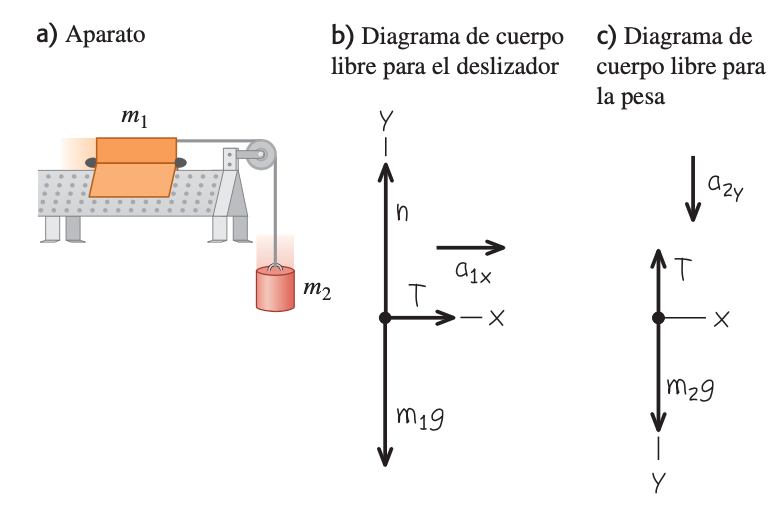
\includegraphics[width=.75\textwidth]{imagenes/imagenes03/T03IM40.png}
	\end{figure}
\end{prob}

\small{Los dos cuerpos tienen diferente movimiento, uno horizontal y el otro vertical.}

\small{Si bien las direcciones de las dos aceleraciones son distintas, sus magnitudes son iguales. Ello se debe a que el cordón no se estira; por lo tanto, los dos cuerpos deberán avanzar distancias iguales en tiempos iguales, y así sus rapideces en cualquier instante dado deberán ser iguales. Cuando las rapideces cambian, lo hacen en la misma cantidad en un tiempo dado, de manera que las aceleraciones de los dos cuerpos deben tener la misma magnitud a. Podemos expresar esta relación así $a_{1_x}=a_{2_y}=a$}

\small{Gracias a esta relación, en realidad sólo tenemos dos incógnitas: $a$ y la tensión $T$}\normalsize{.}

Deslizador: $\begin{cases} \Sigma F_x=T=m_1 a \\ \Sigma F_y=N-m_1g=0 \end{cases}$ peas: $\Sigma F_y=m_2 g-T=m_2 a$

$a=\dfrac {m_2}{m_1+m_2}g;\qquad \qquad T=\dfrac {m_1 m_2}{m_1+m_2}g$


\vspace{4mm}\textbf{Análisis de casos extremos:}
\begin{itemize}
\item $m_1=m_2 \to a=\dfrac g 2 \quad (T=mg/2)\ $.
\item $m_1=0 \to a=g \quad (T=0)\ $, $m_2$ cuerpo libre.
\item $m_2=0 \to a=0 \quad (T=0)\ $, cuerpo $m_1$ en reposo.	
\end{itemize}


\begin{prob}.
	\begin{figure}[H]
	\centering
	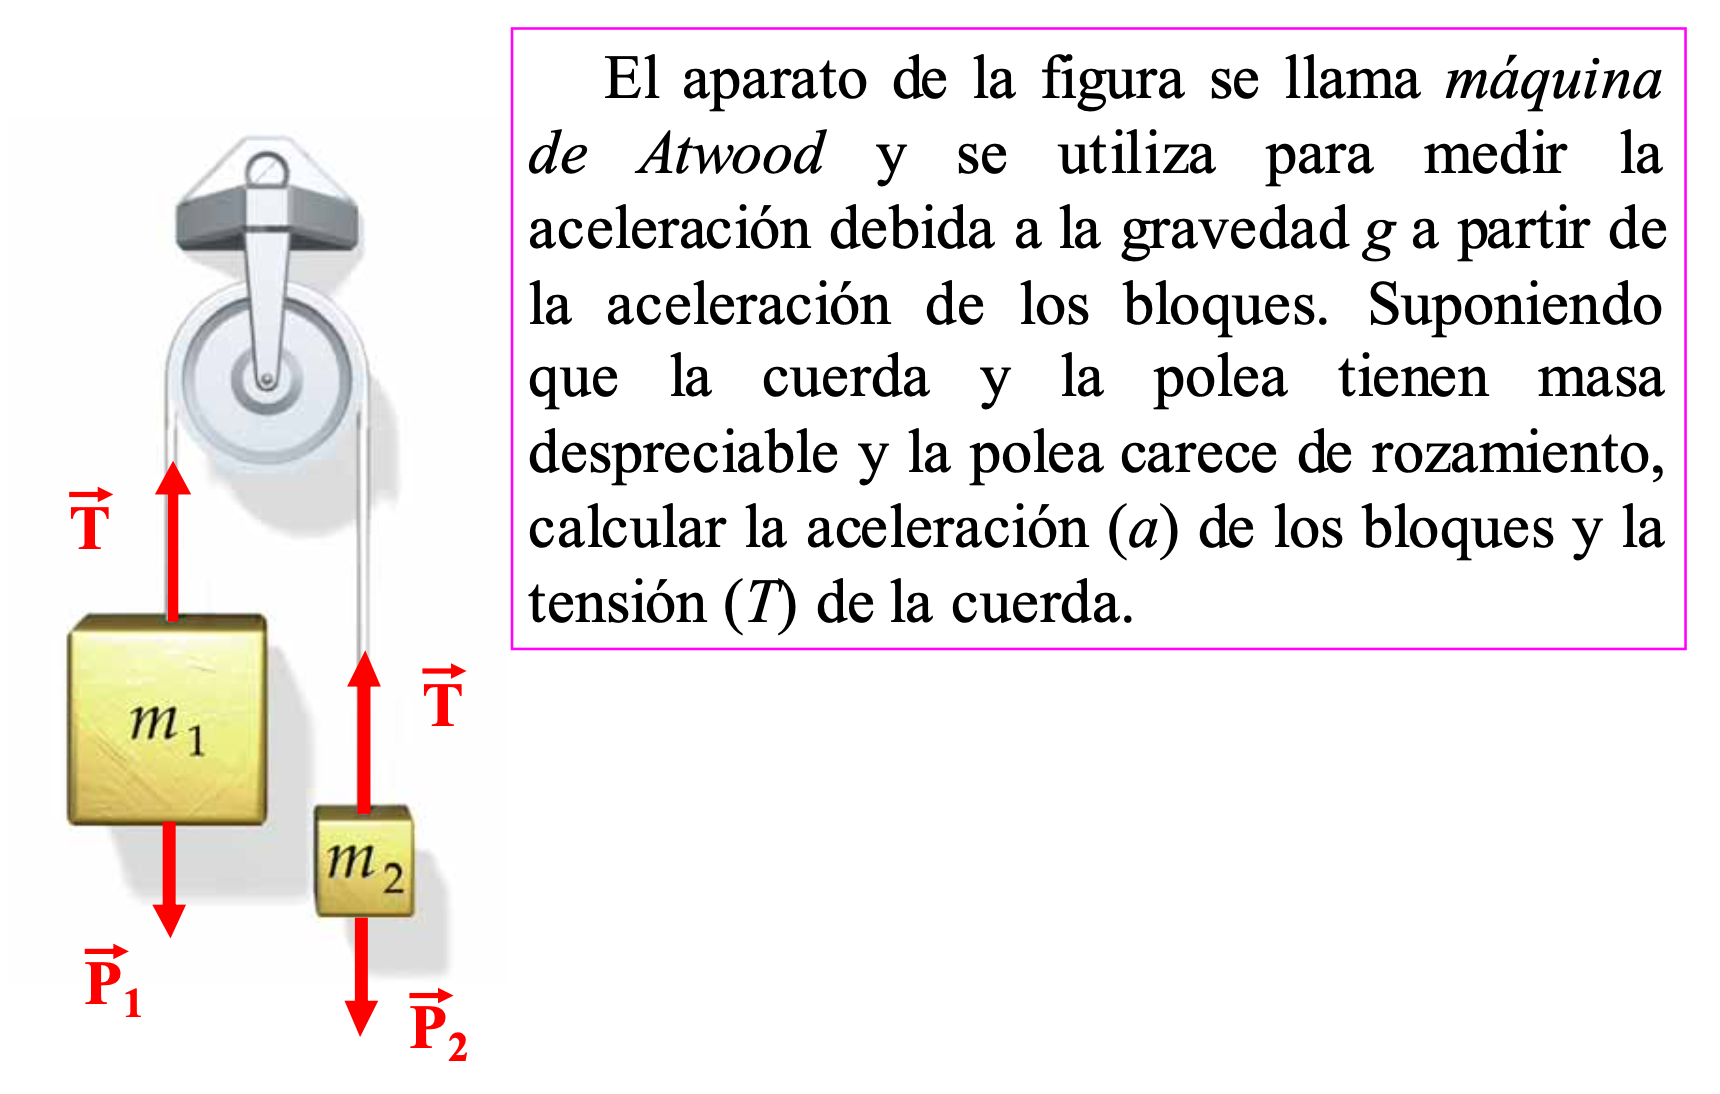
\includegraphics[width=1\textwidth]{imagenes/imagenes03/T03IM22.png}
	\end{figure}
\end{prob}

\vspace{6mm} %*****************************************
\small{\textsf{Se conoce como fuerza de tensión a la fuerza que, aplicada a un cuerpo elástico, tiende a producirle una tensión.}}

\small{\textsf{Las cuerdas, por ejemplo, permiten transmitir fuerzas de un cuerpo a otro. Cuando en los extremos de una cuerda se aplican dos fuerzas iguales y contrarias, la cuerda se pone tensa. Las fuerzas de tensión son, en definitiva, cada una de estas fuerzas que soporta la cuerda sin romperse}}\normalsize{.}

\begin{multicols}{2}
Observado cada cuerpo por separado (diagrama de cuerpo libre).

Elegimos el sentido de giro hacia la masa mayor $m_1$. En principio es arbitrario, si nos equivocamos saldrá $a<0$ lo que indicará que el giro es en el sentido contrario:

\noindent \small{$y \downarrow >0 \to a \downarrow > 0;\; \; y \uparrow < 0 \to a \uparrow < 0$}\normalsize{.}
\begin{figure}[H]
	\centering
	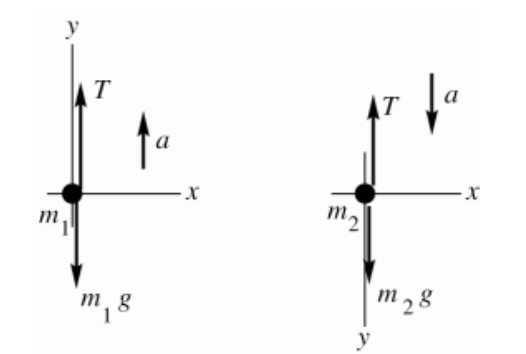
\includegraphics[width=.4\textwidth]{imagenes/imagenes03/T03IM34.png}
	\end{figure}
\end{multicols}


Aplicamos a ambos cuerpos que $\Sigma F=m \ a$:

$\left.
\begin{matrix} 
 m_1 \ g -T =m_1 \ a \\ T - m_2 \ g =m_2 \ a	
\end{matrix}
\right\} \displaystyle \to a=\dfrac{m_2 - m_1}{m_1+,_2} \ g;  \qquad T=\dfrac {2m_1m_2}{m_1+m_2}\ g $
 \textbf{Caso particular:} $m_1=m_2 \to a=0 \quad (T=mg)$, ambos cuerpos estarían en reposo.


\begin{prob}
	En la figura, el motor de peso \textit{w} cuelga de una cadena unida mediante un anillo \textit{O} a otras dos cadenas, una sujeta al techo y la otra a la pared. Calcule las tensiones en las tres cadenas en términos de \textit{w}. Los pesos de las cadenas y el anillo son despreciables.
\end{prob}
	\begin{figure}[H]
	\centering
	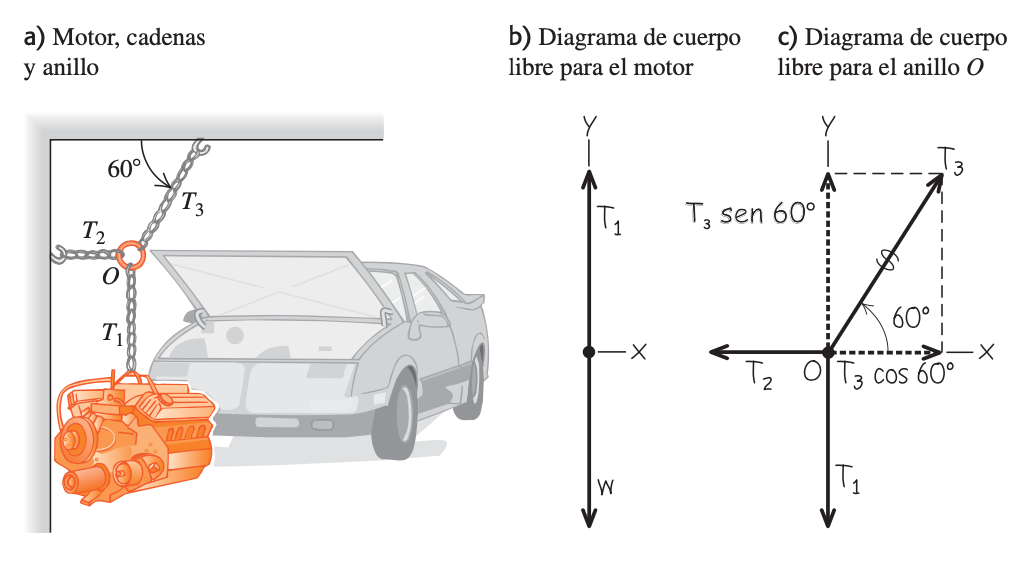
\includegraphics[width=1\textwidth]{imagenes/imagenes03/T03IM38.png}
	\end{figure}

motor: $\Sigma F_y=T_1+\textit{w}=0 \to T_1=\textit{w}$

anillo \textit{O}: $\begin{cases}
\Sigma F_x=T_3 \cos 60^o-T_2=0 \\ \Sigma F_y=T_3 \sin 60^o-T_1=0	
\end{cases} \hspace{-4mm} \to  \begin{cases}
 T_2=0.58 \textit{w} \\ T_3=1.16 \textit{w}	
\end{cases}$

\newpage %**************************************
\begin{prob}.
\begin{multicols}{2}
Un escalador de masa $m_2$ cae por el borde de un glaciar. Afortunadamente está sujeto mediante una cuerda a su compañero, de masa $m_1$ que lleva un piolet. Antes de que éste clave su piolet para detener el movimiento, desliza por la superficie sin rozamiento del glaciar que está inclinada un ángulo $\theta$ respecto de la horizontal. Determinar la aceleración con que cae cada persona y la tensión de la cuerda. El coeficiente de rozamiento entre el escalador del piolet y el bloque de hielo es $\mu$.
	\begin{figure}[H]
	\centering
	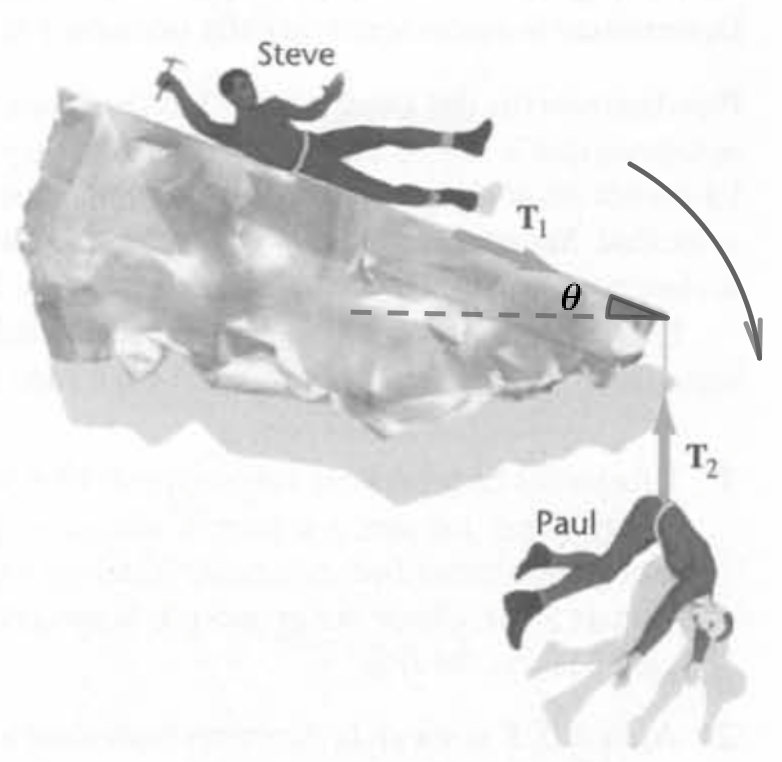
\includegraphics[width=.55\textwidth]{imagenes/imagenes03/T03IM61.png}
	\end{figure}
\end{multicols}
\end{prob}

\begin{multicols}{2}
\begin{figure}[H]
	\centering
	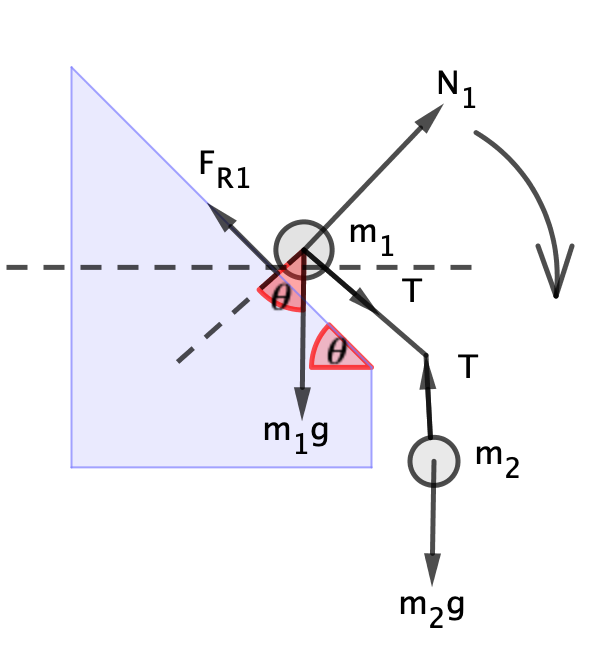
\includegraphics[width=.4\textwidth]{imagenes/imagenes03/T03IM62.png}
	\end{figure}
	
\begin{figure}[H]
	\centering
	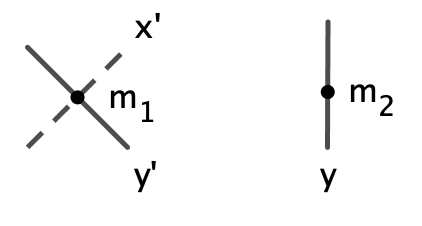
\includegraphics[width=.4\textwidth]{imagenes/imagenes03/T03IM63.png}
	\end{figure}
La cuerda, de masa despreciable, ni se alarga ni se encoge por lo que ambos escaladores se mueven con la misma aceleración
\end{multicols}	

La dirección de movimiento es en los ejes $y'$ e $y$.

$m_1:\quad \begin{cases} \ (reposo) \quad  \Sigma F_{x'}: \quad N-m_1g\cos \theta =0 \\ \ (movto.) \quad \Sigma F_{y'}: \quad T-N\mu+m_1g\sin \theta=m_1 a \end{cases}$

$m_2: \quad \begin{cases} \ (movto.) \quad \Sigma F_y: \quad m_2g-T=m_2 a \end{cases} $

Despejando, se obtiene:

$a=\dfrac{m_1(sin \theta - \mu \cos \theta)+m_2}{m_1+m_2}\ g; \qquad  T=\dfrac {m_1m_2(1-\sin \theta+\mu \cos \theta)}{m_1+m_2}\ g$

\vspace{15mm} %********************************
\begin{prob}
Una camarera empuja una botella de salsa de tomate con masa de $0.45 \mathrm{kg}$ a la derecha sobre un mostrador horizontal liso. Al soltarla, la botella tiene una rapidez de $2.8 \mathrm{ms}{-1}$, pero se frena por la fuerza de fricción horizontal constante ejercida por el mostrador. La botella se desliza 1.0 m antes de detenerse. ?`Qué magnitud y dirección tiene la fuerza de fricción que actúa sobre la botella?
\end{prob}

\vspace{8mm} %********************************
\begin{figure}[H]
	\centering
	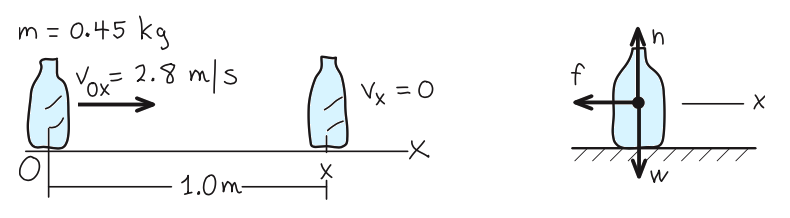
\includegraphics[width=.75\textwidth]{imagenes/imagenes03/T03IM37.png}
	\end{figure}
	
\vspace{-4mm} Del diagrama de fuerzas observamos que la fuerza peso $\mathcal W$ se cancela con la reacción normal del suelo $N$ en el eje y pues no hay movimiento $(a_y=0)$. En el eje $X$, la $a_x$ la encontraremos por cinemática y la única fuerza que actúa es la de rozamiento de la botella con la barra, $F$. Elegimos sentido positivo del eje $X$ el del movimiento de la botella:

$x=x_0+ v_= t + \frac 1 2 a t^2 \; \wedge \; v=v_0+a t$

$x_0=0$, $v_0=2.8\ \mathrm{m s}^{-1}$, $x=1\ \mathrm{m}$ $\quad \to a=-3.9 \mathrm{ms}^{-2}$, negativa, es un movimiento de frenado.

$\Sigma F_x=m a_x \to -F=ma $ $\quad m=0.35\ \mathrm{Kg}$ $\quad F=1.8 \mathrm{N}$

\emph{Las fuerzas de rozamiento siempre se oponen al movimiento.}

\begin{prob}.
\begin{multicols}{2}
Problema del mono y los plátanos. Un mono de $20 \mathrm{kg}$ sujeta firmemente una cuerda ligera que pasa por una polea sin fricción y está atada a un racimo de plátanos de $20 \mathrm{kg}$. El mono ve los plátanos y comienza a trepar por la cuerda para alcanzarlos. a) Al subir el mono, ¿los plátanos suben, bajan o no se mueven? b) Al subir el mono, ¿la distancia entre él y los plátanos disminuye, aumenta o no cambia? c) El mono suelta la cuerda. ¿Qué pasa con la distancia entre él y los plátanos mientras él cae? d) Antes de tocar el suelo, el mono sujeta la cuerda para detener su caída. ¿Qué sucede con los plátanos?
\begin{figure}[H]
	\centering
	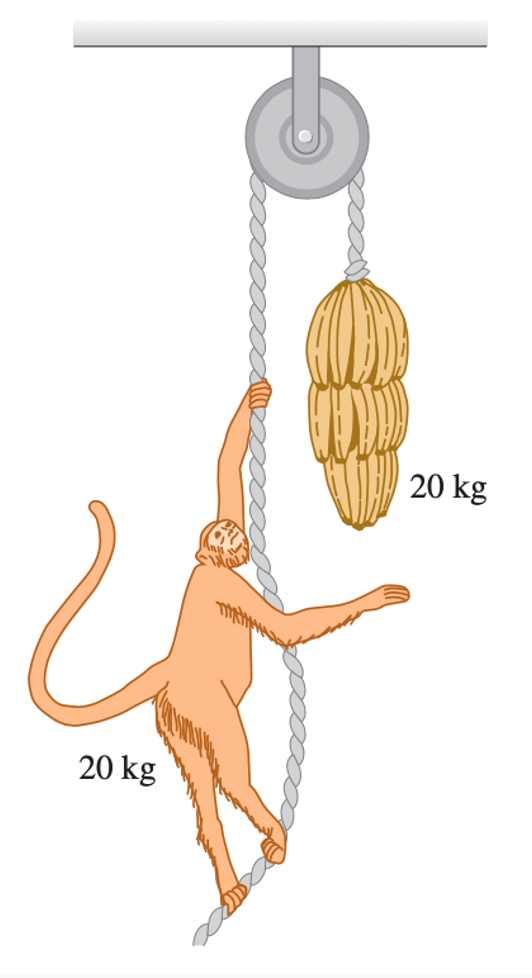
\includegraphics[width=.25\textwidth]{imagenes/imagenes03/T03IM36.png}
	\end{figure}	
\end{multicols}	
\end{prob}

El mono y los plátanos tienen la misma masa y la tensión en la cuerda es la misma. Por tanto, el mono y los plátanos tendrán la misma fuerza neta y, por ello, la misma aceleración, tanto en magnitud como en dirección.

(a) Para que el mono suba, $T> mg$. Los plátanos también suben.

(b) Los plátanos y el mono se mueven con la misma aceleración y la distancia entre ellos permanece constante. 

 (c) Tanto el mono como los plátanos están en caída libre. Tienen la misma velocidad inicial y, a medida que caen, la distancia entre ellos no cambia.

(d) Los plátanos se ralentizarán al mismo ritmo que el mono. Si el mono se detiene, también lo harán los plátanos.

Conclusión: ninguna de estas acciones acerca al mono a los plátanos.
 

\begin{prob}.
	\begin{figure}[H]
	\centering
	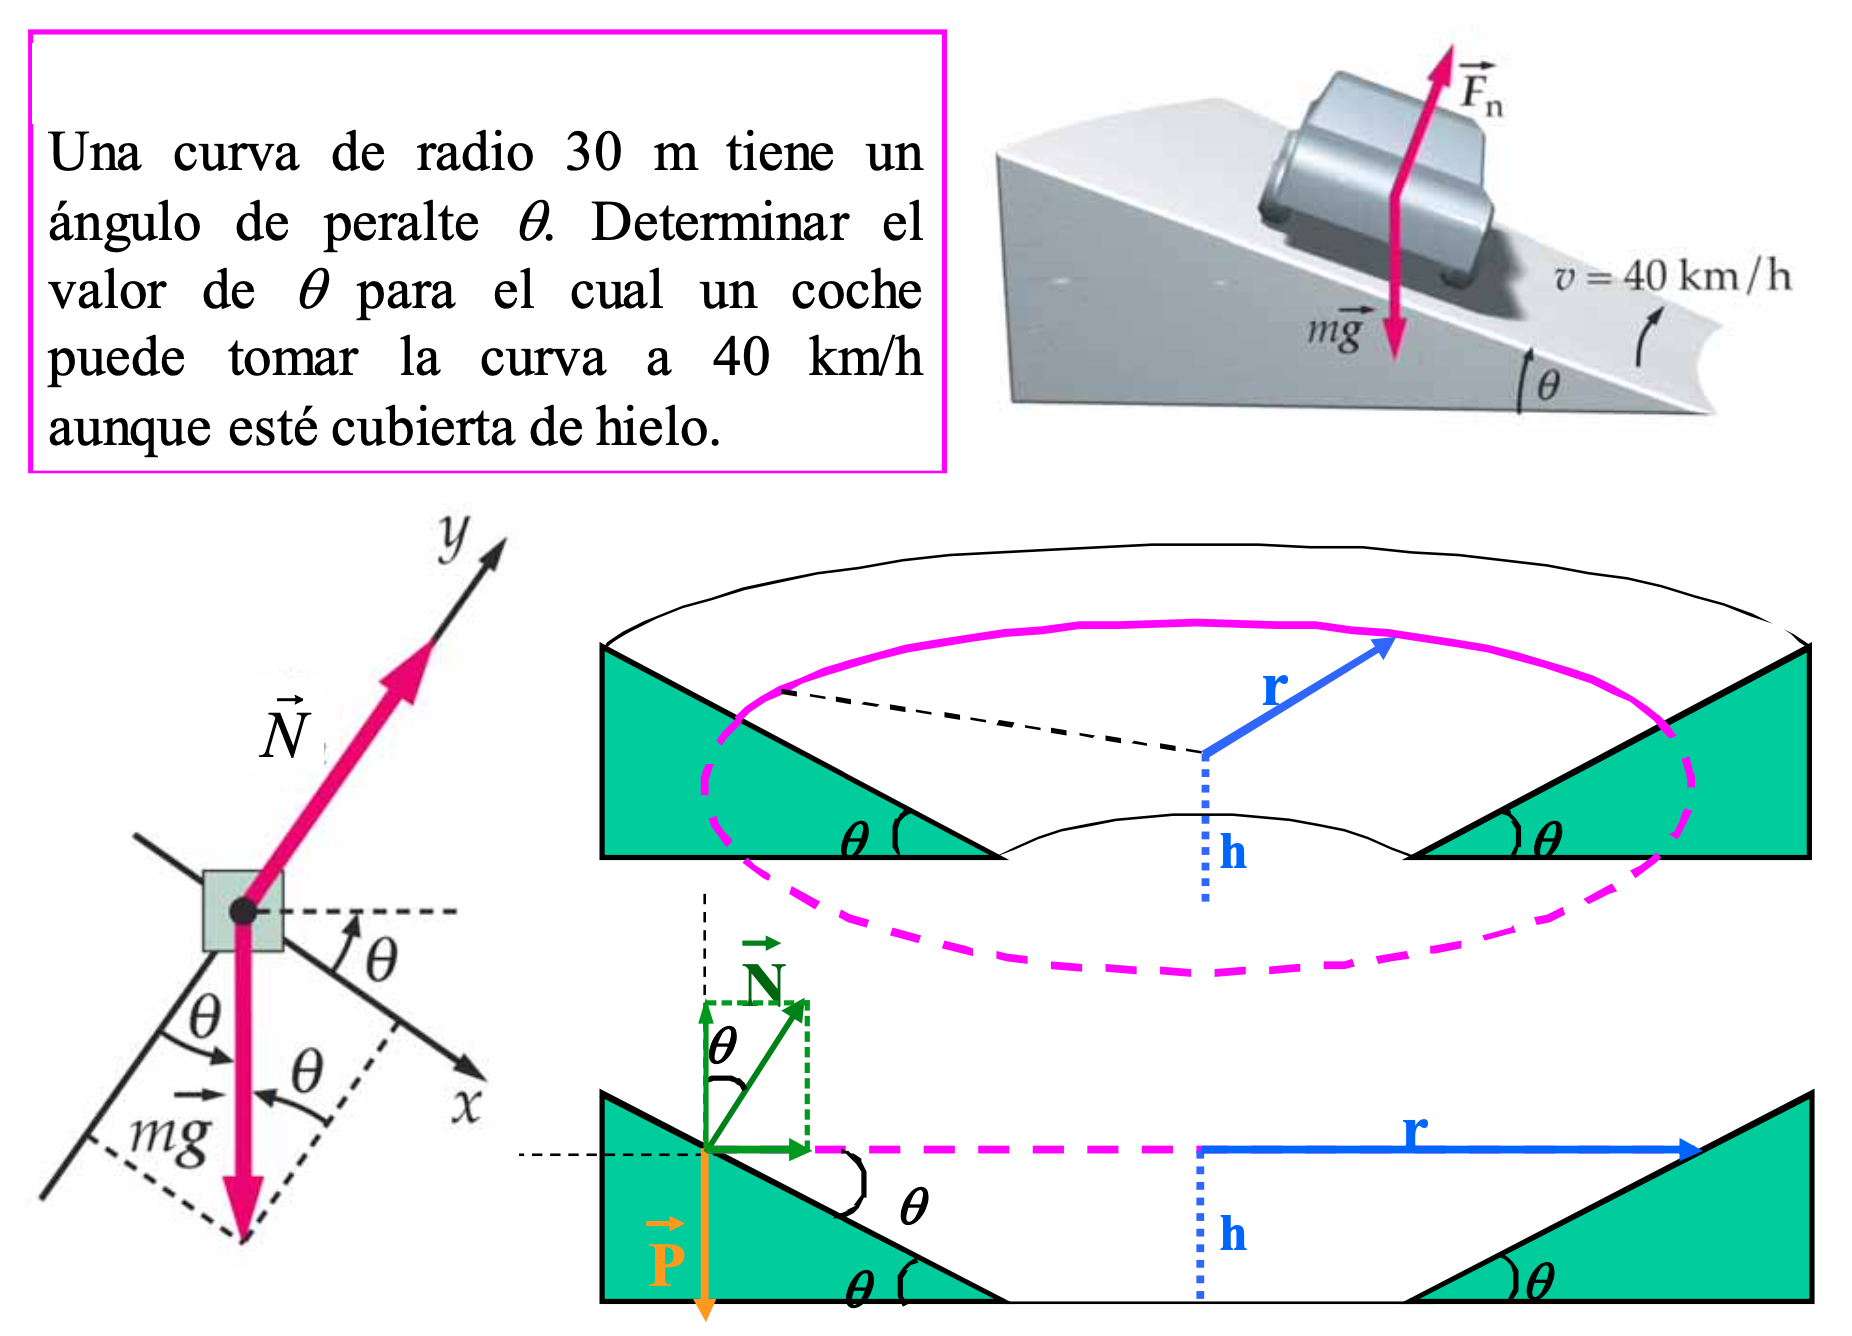
\includegraphics[width=.8\textwidth]{imagenes/imagenes03/T03IM28.png}
	\end{figure}
\end{prob}

\vspace{-4mm} $v=cte \to MCU: \;\; a_x=a_N= {v^2} / r$

$\Sigma F_y=m a_y \to N \cos \theta - mg =0 \to N=\dfrac {mg}{\cos \theta}$

$\Sigma F_x=m a_x\to N \sin \theta = m \dfrac {v^2} r \downarrow \to \;\tan \theta =\dfrac{v^2}{rg}$

Con los datos del problema: $\theta = 22.8^o$






\begin{prob}.
	\begin{figure}[H]
	\centering
	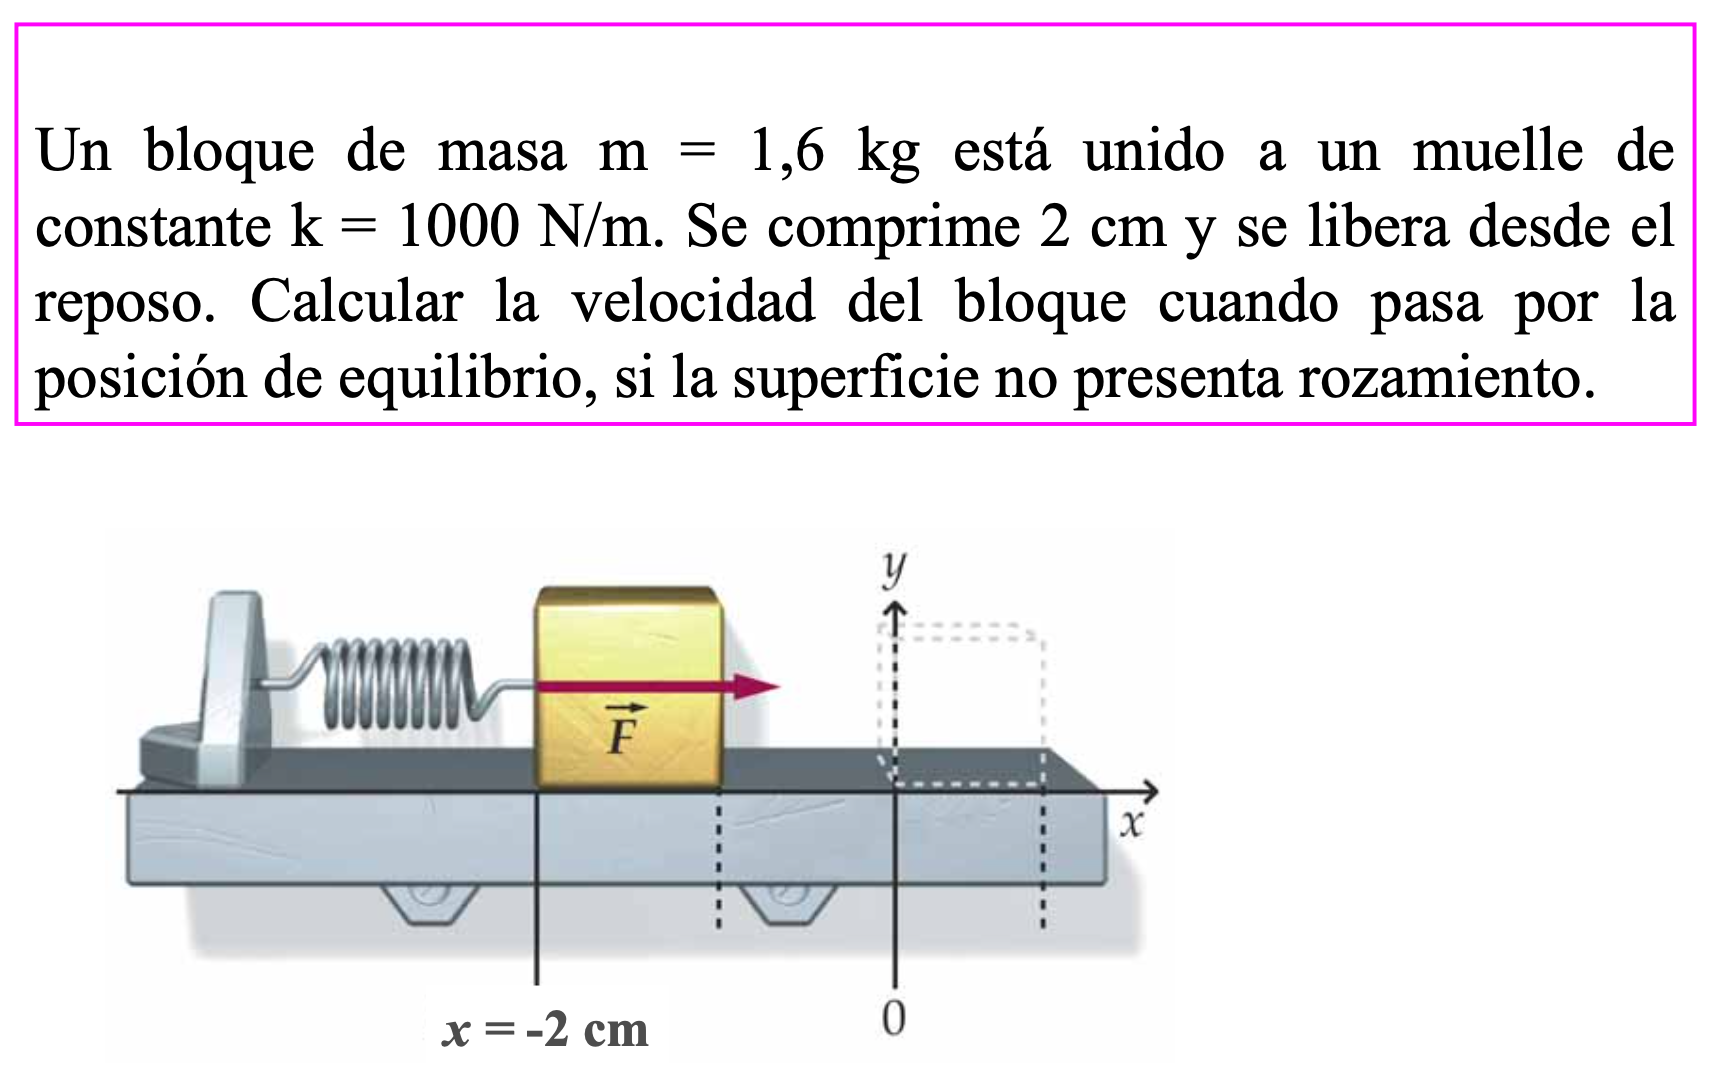
\includegraphics[width=.75\textwidth]{imagenes/imagenes03/T03IM32.png}
	\end{figure}
\end{prob}

El trabajo que realiza el muelle (de masa despreciable) para recuperar su posición original se invierte en aumentar la velocidad del bloque (que desliza sobre el plano sin rozamiento):

$W=\displaystyle \int_0^{x_0} F \dd x=\int_0^{x_0} K x \dd x= \frac 1 2 k x_0^2$

$\Delta \mathcal E_c=\frac 1 2 m v^2 - 0$

$W=\Delta \mathcal E_c \to v=\displaystyle \sqrt{\dfrac k m }\ x_0$


\rule{150 pt}{0.4 pt}

\begin{multicols}{2}
\textbf{Fuerza centrípeta}
\small{!`CUIDADO!: Evite usar ``fuerza centrífuga’’. La figura muestra tanto un diagrama de cuerpo libre correcto para el movimiento circular uniforme (figura a) como un diagrama común incorrecto (figura b). La figura b es incorrecta porque incluye una fuerza adicional hacia afuera de magnitud $m(v^2/R)$ para ``mantener el cuerpo en equilibrio’’. Hay tres razones para no incluir tal fuerza hacia fuera, que solemos llamar \textit{ fuerza centrífuga} (`centrífuga’ significa `que se aleja del centro’). }


\small{En primer lugar, el cuerpo no está en equilibrio; está en movimiento constante con trayectoria circular. Puesto que su velocidad está cambiando constantemente de dirección, el cuerpo está acelerado. }

\small{En segundo lugar, si hubiera una fuerza adicional hacia afuera para equilibrar la fuerza hacia adentro, no habría fuerza neta y el cuerpo se movería en línea recta, no en un círculo.}

\small{Y, en tercer lugar, la cantidad $m(v^2/R)$ no es una fuerza real, no aparece en la (figura a). }

\begin{figure}[H]
	\centering
	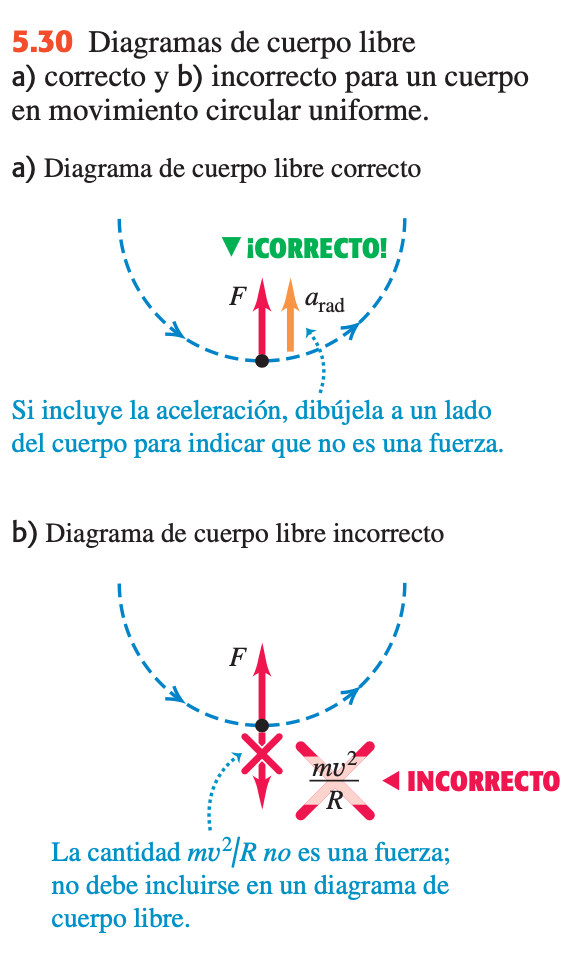
\includegraphics[width=.35\textwidth]{imagenes/imagenes03/T03IM41.png}
	\end{figure}
\end{multicols}
\normalsize{Es} cierto que un pasajero en un automóvil que sigue una curva en un camino horizontal tiende a deslizarse hacia fuera de la curva, como si respondiera a una “fuerza centrífuga” pero, lo que realmente sucede es que el pasajero tiende a seguir moviéndose en línea recta (principio de inercia), y el lado del coche `choca’ contra el pasajero cuando el auto da vuelta. En un marco de referencia inercial no existe ninguna ``fuerza centrífuga’’. No volveremos a mencionar este término, y le recomendamos no usarlo nunca. 

\rule{150 pt}{0.4 pt}

\begin{prob}
Un trineo con masa de $25.0\ \mathrm{kg}$ descansa en una plataforma horizontal de hielo prácticamente sin fricción. Está unido con una cuerda de $5.00\ \mathrm{m}$ a un poste clavado en el hielo. Una vez que se le da un empujón, el trineo da vueltas uniformemente alrededor del poste. Si el trineo efectúa cinco revoluciones completas cada minuto, calcule la fuerza $F$ que la cuerda ejerce sobre él.	
\end{prob}
\begin{multicols}{2}
$MCU: $

$a=a_n=\dfrac {v^2}R=\omega^2 R = $

$=\left(\dfrac {2 \pi}{T}\right)^2 R $

$F=m \ a_N = 34.3 \ \mathrm{N}$
\begin{figure}[H]
	\centering
	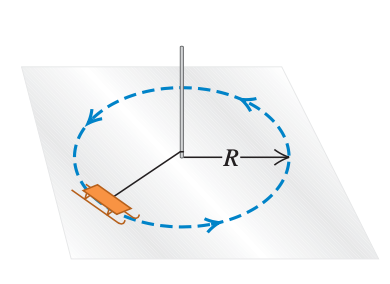
\includegraphics[width=.3\textwidth]{imagenes/imagenes03/T03IM42.png}
	\end{figure}
\end{multicols}

\begin{prob}
	Un inventor propone fabricar un reloj de péndulo usando una lenteja de masa $m$ en el extremo de un alambre delgado de longitud $L$. En vez de oscilar, la lenteja se mueve en un círculo horizontal con rapidez constante $v$, con el alambre formando un ángulo constante $\beta$ con la vertical. Este sistema se llama \textit{péndulo cónico} porque el alambre suspendido forma un cono. Calcule la tensión $F_T$ en el alambre y el periodo $T$ (el tiempo de una revolución de la lenteja) en términos de $\beta$.
\end{prob}
\begin{figure}[H]
	\centering
	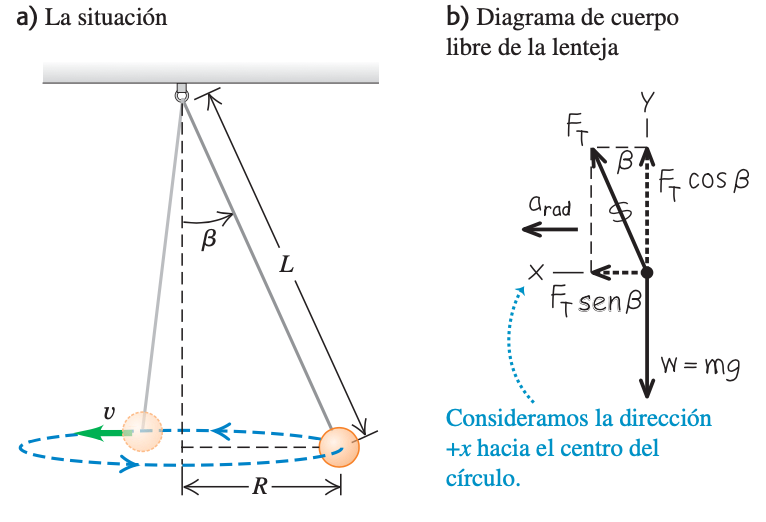
\includegraphics[width=.8\textwidth]{imagenes/imagenes03/T03IM43.png}
	\end{figure}

$a_{rad}=A_N=\omega^2 R=\left( \dfrac {2\pi}{T} \right)^2 R;\qquad L=R \sin \beta; \quad F_T=T$

$\left. \begin{array}{ll}
\Sigma F_x=F \sin \beta = m a_N \\ \Sigma F_y=F \cos \beta -mg=0
 \end{array}\right\} \quad F=\dfrac{mg}{\cos \beta}; \quad \tan \beta=\dfrac{a_N}{g} $

$ a_N=\dfrac{4 \pi L^2 \sin \beta}{T^2}; \quad \tan \beta =\dfrac{4 \pi L^2 \sin \beta}{gT^2}\; \to \;  \quad T=2\pi \ \sqrt{\dfrac{L \cos \beta}{g}}$

\textbf{caso particular:} $\beta=0^o \to T=2\pi \sqrt{\dfrac L g}$, periodo del péndulo simple. \\ %línea en blanco ****************

\begin{prob}.

\begin{multicols}{2}
$\quad$

Un automóvil deportivo va por una curva sin `peralte' de radio $R$. Si el coeficiente de fricción estática entre los neumáticos y la carretera es $\mu_s$, ¿cuál es la rapidez máxima $v_{max}$ con que el conductor puede tomarse la curva sin derrapar?	
\begin{figure}[H]
	\centering
	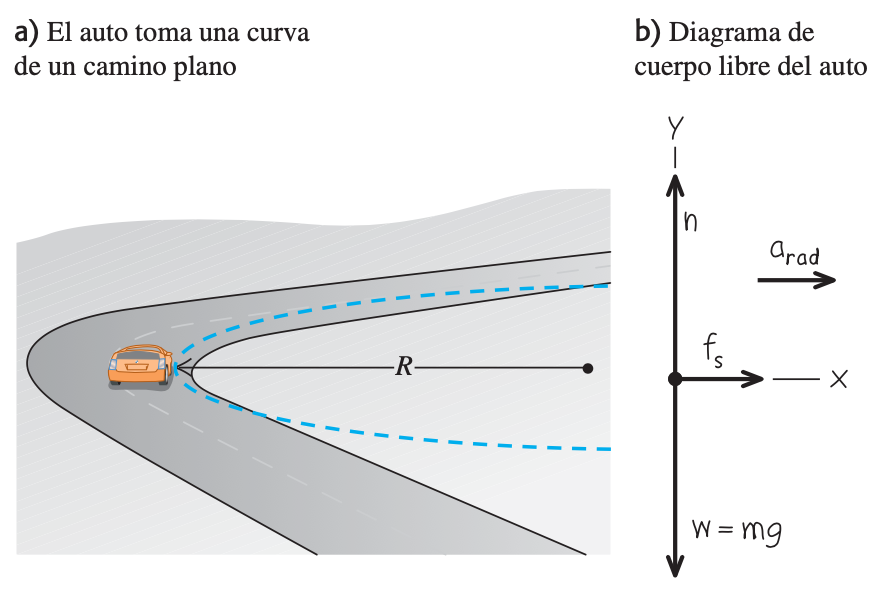
\includegraphics[width=.5\textwidth]{imagenes/imagenes03/T03IM44.png}
	\end{figure}
\end{multicols}
\end{prob}

$\Sigma F_x= m a_N = m \dfrac {v^2}{R} \quad \quad  \Sigma F_y=N-mg=0
  $
 
 La primera ecuación muestra que la fuerza de fricción necesaria para mantener el auto en su trayectoria circular aumenta con la rapidez del auto. No obstante, la fuerza máxima de fricción disponible es
 $F_{max}=\mu_s N =\mu_s m g$, lo cual determinará la velocidad máxima del coche:
 
 $\mu_s m g= m \dfrac {v^2}{R} \to v_{max}=\sqrt{\mu_s g R}$
 
 \small{\textsf{Si la velocidad del coche es menor que $msgR$, la fuerza de fricción requerida es menor que el valor máximo $f_{max} = \mu_s m g$ y el coche puede tomar la curva fácilmente. Si tratamos de tomar la curva con una rapidez mayor que la máxima, el auto aún podrá describir un círculo sin derrapar, pero el radio será mayor y se saldrá de la carretera.}}
 
 \small{\textsf{Cabe señalar que la aceleración centrípeta (normal) máxima es $\mu_s g$. Si se reduce el coeficiente de fricción, la aceleración centrípeta máxima y $v_{max}$ también se reducen. Por ello, es mejor tomar las curvas a menor rapidez si el camino está mojado o cubierto de hielo (pues ambas cuestiones reducen el valor de $\mu_s$)}}\normalsize{.}
 
 \begin{prob}
 Para un automóvil que viaja a cierta rapidez, es posible ``peraltar'' una curva con un ángulo tal que los coches que viajan con cierta rapidez no necesiten fricción para mantener el radio con que dan vuelta. El auto podría tomar la curva aun sobre hielo húmedo. (Las carreras de trineos se basan en la misma idea). Un ingeniero propone reconstruir una curva de modo que un automóvil con rapidez $v$ pueda dar la vuelta sin peligro aunque no haya fricción. ?`Qué ángulo de peralte b debería tener la curva?	
 \end{prob}
 \vspace{-5mm}%*******************************************
\begin{figure}[H]
	\centering
	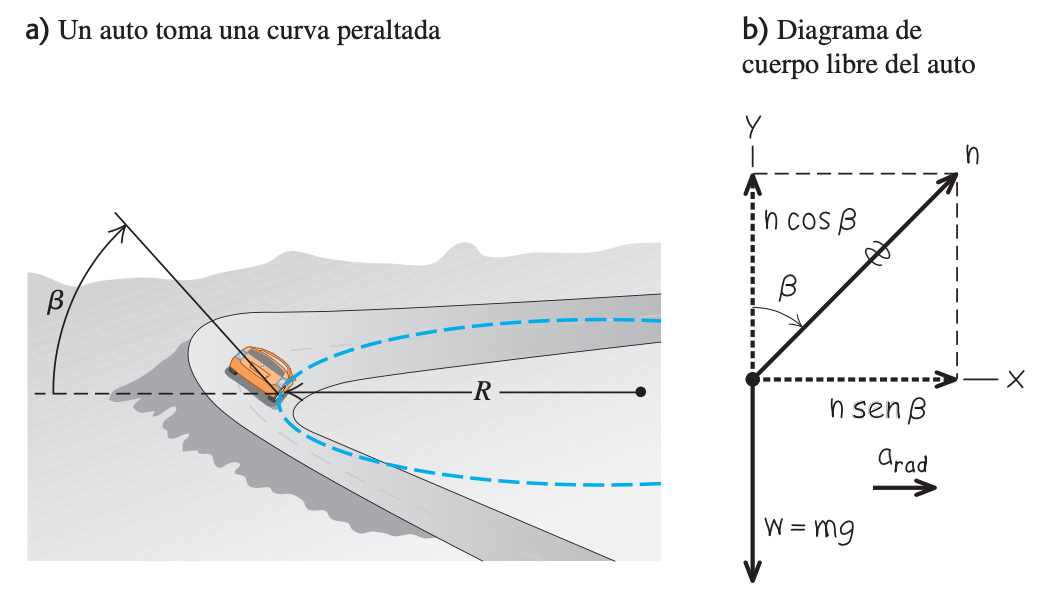
\includegraphics[width=.9\textwidth]{imagenes/imagenes03/T03IM45.png}
	\end{figure}
 
 
 $\left. \begin{array}{ll}
\Sigma F_x= N\sin \beta=m a_N = m \dfrac {v^2}{R} \\ \Sigma F_y=N\cos \beta-mg=0
 \end{array}\right\} \quad N=\dfrac{mg}{\cos \beta};\qquad \tan \beta=\dfrac{a_N}{g}$
 
 $a_N=\dfrac {v^2}{R} \to \quad \tan \beta = \dfrac {v^2}{gR};\qquad \beta=\beta(v,R)$
 

 \begin{prob}.
 \begin{figure}[H]
	\centering
	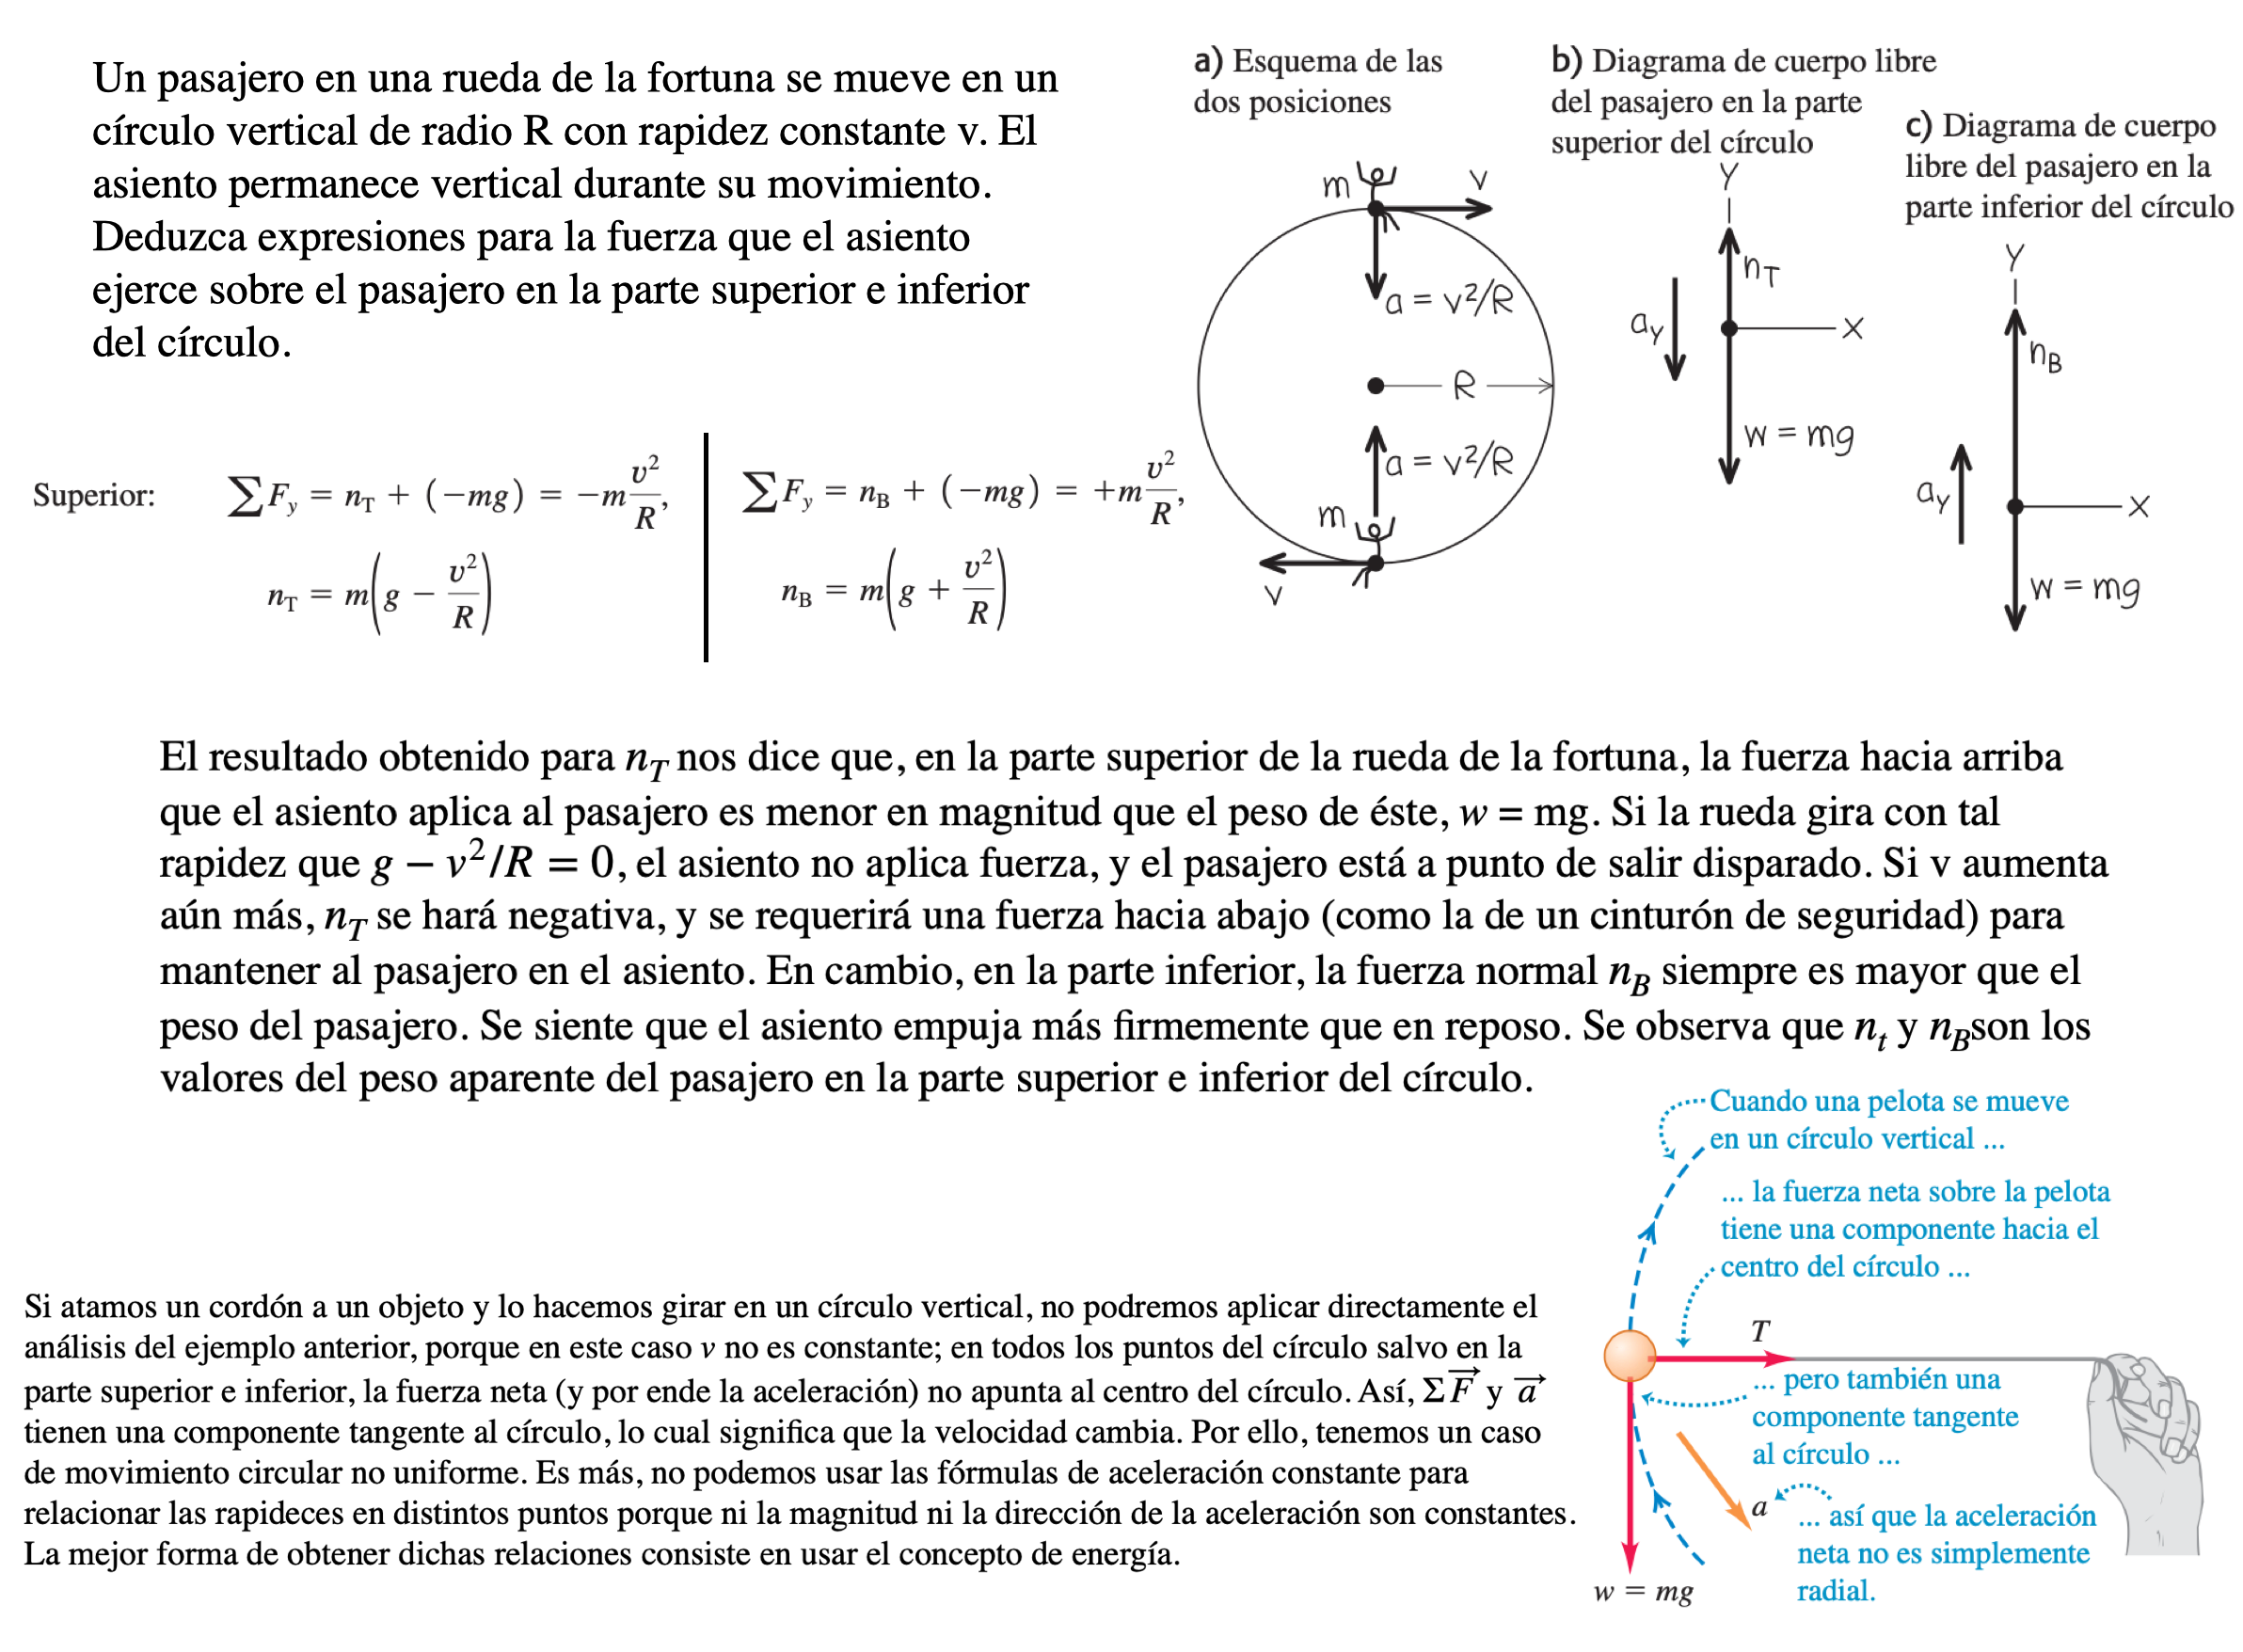
\includegraphics[width=1\textwidth]{imagenes/imagenes03/T03IM46.png}
	\end{figure}
 \end{prob}
 

\begin{prob}
Un disco de hockey se desliza sobre una mesa de aire, sin fricción; sus coordenadas son $(x,y)$ y sobre él actúa una fuerza conservativa descrita por la función de energía potencial	: $\mathcal E_p(x,y) )= \frac 1 2 k(x^2+y^2)$. Deduzca una expresión para la fuerza que actúa sobre el disco y obtenga una expresión para el módulo de la fuerza en función de la posición.
\end{prob}

En dos dimensione: $\ F_x=-\pdv{x}\mathcal E_p=-Kx; \quad F_y=-\pdv{y}\mathcal E_p=-Ky$

Luego: $\overrightarrow{F}=F_x \vec i + F_y \vec j = -k \ (x\vec i + y \vec j)=-k \ \overrightarrow{r}$

\textcolor{gris}{La fuerza es central, $\overrightarrow{F}=-K \vec r$, luego es conservativa.}

$F=\abs{\vec F}=\sqrt{F_x^2+F_y^2}=k\sqrt{x^2+y^2}=k\ r$, con $r$ la distancia del disco al origen.

\begin{prob}
En cierta región del espacio, la fuerza que actúa sobre un electrón es $\vec F=  Cx\vec j$, donde $C$ es una constante positiva. El electrón se mueve en sentido antihorario en un cuadrado sobre el plano $xy$ . Las esquinas del cuadrado están en $(x, y):\  (0, 0),\ (L, 0),\ (L, L) \text{ y } (0, L)$. Calcule el trabajo de $\vec F$ sobre el electrón durante una vuelta. ¿Esta fuerza es conservativa o no conservativa?	
\end{prob}

\begin{multicols}{2}
$W=\displaystyle \int_{cuadrado}\vec F \cdot \dd \vec l$. 

Calcularemos el trabajo tramo a tramo y sumaremos todos los resultados obtenidos.
De $(0,0)\ a \ (L,0)$, el $W=0$, pues $\vec F \bot \dd \vec l$, lo mismo ocurre para el trabajo desde $(L,L)$ hasta $(=,L)$.

Desde $(=,L)$ hasta $(0,0)$, también es $W=o$, pues $\vec F=0$
	\begin{figure}[H]
	\centering
	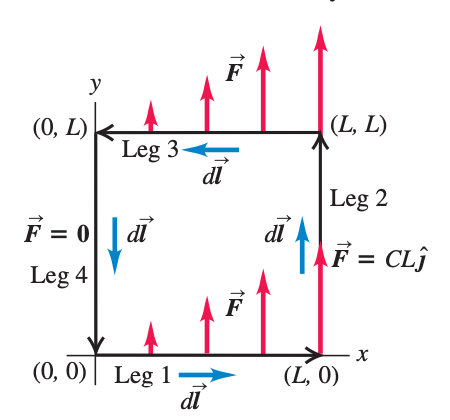
\includegraphics[width=.4\textwidth]{imagenes/imagenes03/T03IM53.png}
	\end{figure}
\end{multicols}
Trabajo desde $(L,O)$ hasta $(L,L)$. En este tramo la fuerza $\vec F$ es paralela al desplazamiento $\dd \vec l= \dd y\ \vec j$, luego $\vec F \cdot \dd \vec l = C\ L \ \dd y$

Así, $\ \displaystyle W_{(L,0) \to (L,L)} = \int_C \vec F \cdot \dd \vec l = \int_{y=0}^{y=L} C L \ \dd y= C L \ \left[ \eval{y}_0^L \right.=C L^2$

$W=0+CL^2+0+0=CL^2$

Como el trabajo desarrollado a lo largo de un camino cerrado (espira cuadrada) no ha resultado ser cero, entonces, la fuerza no es conservativa (no se deriva de una función escalar --potencial.) 


\begin{prob}
Curva peraltada con rozamiento.	
\end{prob}

Las fuerzas que aparecen son el peso $mg$, la reacción normal del plano $\vec N$

La aceleración normal $a_n$ no es paralelo al plano, es horizontal. Ver figura adjunta:

\begin{figure}[H]
	\centering
	\includegraphics[width=1\textwidth]{imagenes/imagenes03/T03IM56.png}
	\end{figure}

\noindent $\Sigma F_y:\;\; N\cos \theta-F_R \sin \theta -mg=0;\qquad \Sigma F_x:\;\; N\sin \theta+F_R \cos \theta =m \dfrac {v^2}{R}$

El vehículo deslizará en la dirección radial cuando su velocidad sea tal que $F_R=\mu N$:

$F_R=\mu N \ \to \ \begin{cases} \ N(\cos \theta-\mu \sin \theta)=mg \\ \ N(\sin \theta+\mu \cos \theta)=mv^2/R \end{cases} $


De donde, la velocidad máxima que puede llegar el vehículo es: 

$$ v=\sqrt{Rg \ \dfrac {\sin \theta + \mu \cos \theta} {\cos \theta - \mu \sin \theta}} $$

\textbf{Caso límite:} Si no hay rozamiento, $\mu=0 \to v= \sqrt{RG\tan \theta}$, ecuación que ya habíamos obtenido en un problema anterior al analizar una curva peraltada sin rozamiento.


\begin{prob}
Una partícula de $8 \ \mathrm{g}$  de masa se deja caer desde el reposo bajo la influencia de su propio peso	 en un medio en que existe una fuerza retardadora $\vec F=-9.8\times 10^{-3}\ \vec v\  \mathrm{N}$ , si $v$ se expresa en $\mathrm{ms}^{-1}$. Al cabo de $3\ \mathrm{s}$  toca el suelo. ?`A qué velocidad lo hace y desde qué altura se soltó?
\end{prob}

\begin{multicols}{2}
$v_0=0;\ t=3 \ \mathrm{s};\ m=8\times 10^{-3}\ \textrm{Kg}$

$\overrightarrow{F_R}=9.8\times 10^{-3}\ \vec v=Av\ \vec j$

$ A=9.8\times 10^{-3} \dfrac{\mathrm{N}}{\mathrm{ms}^{-1}}=$

$=9.8\times 10^{-3}\ \mathrm{kgs}^{-1}$
\begin{figure}[H]
	\centering
	\includegraphics[width=.25\textwidth]{imagenes/imagenes09/T09IM11.png}
\end{figure}		
\end{multicols}
$F_T=F_R-mg=Av-mg=ma \to a=\dfrac Am v - g =\displaystyle \dv{v}{t}$

$\boldsymbol{\frac m A} \displaystyle  \ \int_{v_0=0}^{v} {\dfrac{\boldsymbol{\frac A m} \dd v}{\frac A m v - g}}=\int_0^t \dd t \to $ 
$\quad \frac m A  \displaystyle \eval{ \ln(\frac A m v - g) }_0^v=t$

$\dfrac m A \ln \left( 1-\dfrac{Av}{mg} \right)=t \ \to \quad \boxed{\boldsymbol{v=\dfrac{mg}{A} \left( e\ ^{\dfrac {At}{m} }-1 \right)}}$

$v=\displaystyle \dv{y}{t} \to \dd y= v\ \dd t; \qquad t=0 \to y(0)=0;\quad t\to y=0$

$-H=\displaystyle \int_{H}^0 \dd y = \int_0^t \dfrac{mg}{A} \left( e\ ^{\dfrac {At}{m} }-1 \right) \dd t =
   \boldsymbol{\dfrac m A} \dfrac{mg}{A}  \int_0^t  \boldsymbol{\dfrac A m} e\ ^{\dfrac {At}{m} } \dd t  \ -
   \dfrac{mg}{A} \int_0^t  \dd t 
$

$\boxed{ \boldsymbol{ H= \dfrac{mg}{A} \left[ t - \dfrac m A \left( e^{\dfrac{At}{m}}-1 \right) \right] } }$

Sustituyendo los datos del problema, obtenemos: 

$v= \cdots \ \mathrm{ms}^{-1}; \qquad H= \cdots \ \mathrm{m}$

\rightline{\textsf{\textcolor{DarkBlue}{--- Inacabado --- \small{comporbar soluciones}\normalsize{.}}}}



\newpage %********************************

 \begin{myblock}{Fuerzas fundamentales de la naturaleza}
 
 \begin{small}
 Hemos visto fuerzas de varios tipos ---peso, tensión, fricción, resistencia de fluidos y la fuerza normal--- y veremos otras más al seguir estudiando física. Pero, ?`cuántas clases distintas de fuerzas hay? Actualmente, se considera que todas las fuerzas son expresiones de tan solo cuatro clases de fuerzas o interacciones fundamentales entre las partículas. Dos de ellas las conocemos por la experiencia cotidiana; las otras dos implican interacciones entre partículas subatómicas que no podemos observar directamente con nuestros sentidos. 

\vspace{2mm} Las \textbf{interacciones gravitacionales} incluyen la fuerza familiar del peso, que se debe a la acción de la atracción gravitacional terrestre sobre un cuerpo. La mutua atracción gravitacional entre las diferentes partes de la Tierra mantienen a nuestro planeta unido. Newton demostró que la atracción gravitacional del Sol mantiene a la Tierra en su órbita casi circular en torno al Sol. 

\vspace{2mm} La otra clase cotidiana de fuerzas, las \textbf{interacciones electromagnéticas}, incluye las fuerzas eléctricas y magnéticas. Si nos frotamos un peine por el cabello, al final el peine tendrá una carga eléctrica; es posible usar la fuerza eléctrica para atraer trocitos de papel. Todos los átomos contienen carga eléctrica positiva y negativa, así que átomos y moléculas pueden ejercer fuerzas eléctricas unos sobre otros.  Las fuerzas de contacto, incluidas la normal, la de fricción y la de resistencia de fluidos, son la combinación de todas estas fuerzas ejercidas sobre los átomos de un cuerpo por los átomos de su entorno. Las fuerzas magnéticas, como las que se dan entre imanes o entre un imán y un trozo de hierro, son realmente el resultado de cargas eléctricas en movimiento. Por ejemplo, un electroimán causa interacciones magnéticas porque las cargas eléctricas se mueven por sus alambres. 

\vspace{2mm} En el nivel atómico o molecular, las fuerzas gravitacionales no son importantes porque las fuerzas eléctricas son muchísimo más intensas: la repulsión eléctrica entre dos protones a cierta distancia es $10^{35}$ veces más fuerte que su atracción gravitacional. Sin embargo, en cuerpos de tamaño astronómico las cargas positivas y negativas suelen estar presentes en cantidades casi idénticas, y las interacciones eléctricas resultantes casi se anulan. Por ello, las interacciones gravitacionales son la influencia dominante en el movimiento de los planetas y en la estructura interna de las estrellas. 

\vspace{2mm} Las otras dos clases de interacciones son menos conocidas. La \textbf{interacción fuerte} mantiene unido el núcleo de un átomo. Los núcleos contienen neutrones (eléctricamente neutros) y protones (con carga positiva). La fuerza eléctrica entre protones hace que se repelan mutuamente; la enorme fuerza de atracción entre las partículas nucleares contrarresta esta repulsión y mantiene el núcleo estable. En este contexto, la interacción fuerte también se denomina fuerza nuclear fuerte; tiene un alcance mucho menor que las interacciones eléctricas, pero es mucho más fuerte dentro de ese alcance. La interacción fuerte juega un papel fundamental en las reacciones termonucleares que ocurren en el núcleo del Sol, y que generan el calor y su luz. 

\vspace{2mm} Por ultimo, tenemos la \textbf{interacción débil} cuyo alcance es tan pequeño que es relevante sólo a una escala de núcleo o menor. La interacción débil causa una forma común de radioactividad, llamada desintegración beta, en la que un neutrón de un núcleo radioactivo se transforma en protón al tiempo que expulsa un electrón y una partícula casi sin masa llamada antineutrino electrónico. La interacción débil entre un antineutrino y la materia ordinaria es tan tenue que el antineutrino fácilmente podría atravesar una pared de plomo ¡`de un millón de kilómetros de espesor! 

\vspace{2mm} En la década de 1960 los físicos elaboraron una teoría que describe las interacciones electromagnética y débil, como aspectos de una sola interacción electrodébil. Esta teoría ha superado todas las pruebas experimentales a las que se ha sometido, lo cual motivó a los físicos a realizar intentos similares que describan las interacciones fuerte, electromagnética y débil dentro de una sola gran teoría unificada (GUT), y se han dado ciertos pasos hacia una posible unificación de todas las interacciones en una teoría de todo (TOE). Tales teorías aún son especulativas, y hay muchas preguntas sin respuesta en este campo de investigación tan activo. 
	
 \end{small}

\end{myblock}
 
 
 
 
 
